% =====================================================================
%  Nader Belhadj -- PhD thesis (ENSI, University of Manouba)
%  Main file. Compile: pdfLaTeX + BibTeX (Overleaf default).
% =====================================================================
\documentclass[12pt,a4paper,oneside,openany]{report}
% =====================================================================
%  Preamble -- Belhadj PhD thesis
%  Compiles with pdfLaTeX (Overleaf default) or XeLaTeX / LuaLaTeX.
% =====================================================================
\usepackage{iftex}
\ifPDFTeX
  \usepackage[T1]{fontenc}
  \usepackage[utf8]{inputenc}
  \usepackage{lmodern}
\else
  \usepackage{fontspec}
\fi
\usepackage[english]{babel}
\usepackage{microtype}
\usepackage[a4paper,top=2.6cm,bottom=2.6cm,inner=3.0cm,outer=2.5cm,
            headheight=15pt,headsep=0.8cm,footskip=1.1cm]{geometry}
\usepackage{setspace}
\setstretch{1.3}
\raggedbottom
\setlength{\parskip}{0pt}
\setlength{\emergencystretch}{2.5em}
\hyphenation{Table Tables Figure Figures Section Sections Chapter Chapters Equation Equations Appendix Algorithm DOTS TOPORET RETFound GraphSAGE}
\widowpenalty=10000
\clubpenalty=500

% ---------------------------------------------------------------- maths
\usepackage{amsmath,amssymb,bm}
\numberwithin{equation}{chapter}

% ---------------------------------------------------------------- floats
\usepackage{graphicx}
\usepackage{booktabs,tabularx,longtable,multirow,array,makecell}
\usepackage[table]{xcolor}
\usepackage{tikz}
\usetikzlibrary{arrows.meta,positioning,fit,calc,shapes.geometric,backgrounds}
\tikzset{every picture/.append style={execute at begin picture={\setstretch{1.0}}}}
\usepackage{pgfplots}
\pgfplotsset{compat=1.18}
\usepackage{caption}
\captionsetup{font=small,labelfont=bf,labelsep=endash,justification=justified,
              singlelinecheck=true,skip=6pt}
\captionsetup[figure]{position=bottom}
\captionsetup[table]{position=top}
\usepackage{subcaption}
\usepackage{float}
\usepackage[ruled,vlined,linesnumbered,algochapter]{algorithm2e}
\SetAlgoCaptionSeparator{\unskip~--}
\renewcommand{\listalgorithmcfname}{List of Algorithms}
\SetAlFnt{\small}
\usepackage[section]{placeins}
\usepackage{flafter}
\usepackage{needspace}
\usepackage{pdflscape}
\usepackage{afterpage}
\usepackage{etoolbox}
\AtBeginEnvironment{table}{\setstretch{1.0}}
\AtBeginEnvironment{figure}{\setstretch{1.0}}
\renewcommand{\topfraction}{0.9}
\renewcommand{\bottomfraction}{0.8}
\renewcommand{\textfraction}{0.07}
\renewcommand{\floatpagefraction}{0.75}
\setcounter{topnumber}{3}
\setcounter{totalnumber}{4}
\setlength{\textfloatsep}{14pt}
\setlength{\floatsep}{12pt}
\setlength{\intextsep}{12pt}
\renewcommand{\arraystretch}{1.15}
\setlength{\tabcolsep}{5pt}

% A short italic note placed directly under a table (never repeats "Table X").
\newcolumntype{P}[1]{>{\raggedright\arraybackslash}p{#1}}
\newcommand{\tabnote}[1]{\par\vspace{3pt}{\footnotesize\itshape #1\par}}

% ---------------------------------------------------------------- lists, misc
\usepackage{enumitem}
\setlist{itemsep=2pt,topsep=4pt}
\usepackage{csquotes}
\usepackage{pifont}
\newcommand{\cmark}{\ding{51}}
\newcommand{\xmark}{\ding{55}}
\usepackage{url}

% ---------------------------------------------------------------- Unicode in text
\usepackage{newunicodechar}
\newunicodechar{≤}{\ensuremath{\leq}}
\newunicodechar{≥}{\ensuremath{\geq}}
\newunicodechar{≈}{\ensuremath{\approx}}
\newunicodechar{×}{\ensuremath{\times}}
\newunicodechar{±}{\ensuremath{\pm}}
\newunicodechar{→}{\ensuremath{\to}}
\newunicodechar{−}{\ensuremath{-}}

% ---------------------------------------------------------------- colours
\definecolor{axisR}{HTML}{1F4E79}
\definecolor{axisRf}{HTML}{D6E6F5}
\definecolor{axisS}{HTML}{1B7A4E}
\definecolor{axisSf}{HTML}{D9F0E3}
\definecolor{axisO}{HTML}{6B3D8C}
\definecolor{axisOf}{HTML}{EADCF3}
\definecolor{failred}{HTML}{A32020}
\definecolor{failf}{HTML}{F8D6D6}
\definecolor{okgreen}{HTML}{1B7A4E}
\definecolor{okf}{HTML}{D9F0E3}
\definecolor{limred}{HTML}{C0392B}
\definecolor{navy}{HTML}{16324F}
\definecolor{fusion}{HTML}{B35C00}
\definecolor{fusionf}{HTML}{FCE8D2}

% ---------------------------------------------------------------- headings
\usepackage{titlesec}
\titleformat{\chapter}[display]
  {\normalfont\centering}
  {\large\scshape\color{navy}\chaptertitlename\ \thechapter}
  {6pt}
  {\titlerule[0.6pt]\vspace{8pt}\LARGE\bfseries\color{navy}}
  [{\vspace{6pt}\titlerule[0.6pt]}]
\titleformat{name=\chapter,numberless}[display]
  {\normalfont\centering}
  {}
  {0pt}
  {\titlerule[0.6pt]\vspace{8pt}\LARGE\bfseries\color{navy}}
  [{\vspace{6pt}\titlerule[0.6pt]}]
\titlespacing*{\chapter}{0pt}{-24pt}{22pt}
\titleformat{\section}{\normalfont\Large\bfseries\color{navy}\raggedright}{\thesection}{0.8em}{}
\titleformat{\subsection}{\normalfont\large\bfseries\raggedright}{\thesubsection}{0.8em}{}
\titleformat{\subsubsection}{\normalfont\normalsize\bfseries}{\thesubsubsection}{0.8em}{}
\titlespacing*{\section}{0pt}{18pt}{8pt}
\titlespacing*{\subsection}{0pt}{13pt}{6pt}
\titlespacing*{\paragraph}{0pt}{7pt}{0.8em}
\setcounter{secnumdepth}{2}
\setcounter{tocdepth}{2}

% Chapter epigraph: \epigraph{quote}{source}
\newcommand{\epigraph}[2]{%
  \begin{flushright}\begin{minipage}{0.72\textwidth}\raggedleft\small
  \textit{#1}\par\vspace{3pt}--- #2\end{minipage}\end{flushright}\vspace{10pt}}

% ---------------------------------------------------------------- headers
\usepackage{fancyhdr}
\newif\ifinappendix
\renewcommand{\chaptermark}[1]{\markboth{%
  \ifinappendix Appendix~\thechapter\else Chapter~\thechapter\fi.\ #1}{}}
\renewcommand{\sectionmark}[1]{\markright{\thesection\quad #1}}
\fancypagestyle{thesis}{%
  \fancyhf{}%
  \fancyhead[L]{\small\itshape\nouppercase{\leftmark}}%
  \fancyfoot[C]{\small\thepage}%
  \renewcommand{\headrulewidth}{0.4pt}}
\fancypagestyle{plain}{\fancyhf{}\fancyfoot[C]{\small\thepage}\renewcommand{\headrulewidth}{0pt}}

% ---------------------------------------------------------------- TOC / lists
\usepackage[titles]{tocloft}
\renewcommand{\cftchapfont}{\bfseries}
\renewcommand{\cftchappagefont}{\bfseries}
\setlength{\cftbeforechapskip}{6pt}
\renewcommand{\cftdot}{.}
\setlength{\cftfignumwidth}{3.2em}
\setlength{\cfttabnumwidth}{3.2em}

% Group headings inside the List of Figures / List of Tables
\newcommand{\listgroup}[2]{\addtocontents{#1}{\protect\addvspace{9pt}\protect\noindent\protect\parbox{\protect\linewidth}{\protect\raggedright\protect\small\protect\bfseries\protect\color{navy}\protect\strut#2\protect\strut}\protect\par\protect\nopagebreak\protect\addvspace{4pt}\protect\nopagebreak}}
\newcommand{\lofgroup}[1]{\listgroup{lof}{#1}}
\newcommand{\lotgroup}[1]{\listgroup{lot}{#1}}

% ---------------------------------------------------------------- links (last)
\usepackage[hidelinks,bookmarksnumbered,bookmarksopen]{hyperref}
\hypersetup{
  pdftitle={Deep Learning-Based Prediction of Disease Progression Using Medical Imaging: An Application to Diabetology},
  pdfauthor={Nader Belhadj},
  pdfsubject={Doctoral Thesis in Computer Science -- Artificial Intelligence},
  pdfkeywords={diabetic retinopathy, GraphSAGE, persistent homology, CORAL, clinical AI safety, RETFound}}
\usepackage[nameinlink,capitalise,noabbrev]{cleveref}
\crefname{equation}{Equation}{Equations}
\Crefname{equation}{Equation}{Equations}
\crefname{appendix}{Appendix}{Appendices}

\graphicspath{{img/}{figures/}}

% ------------------------------------------------------------------
% Values that must come from the evaluation outputs (tools/verify_h3a.py).
% Until the script is run, they are printed in red and a warning is issued.
% ------------------------------------------------------------------
\newcommand{\missingvalue}[1]{\textcolor{red}{\textbf{[#1]}}%
  \PackageWarningNoLine{thesis}{Missing value #1: run tools/verify_h3a.py}}
\newcommand{\refT}{\missingvalue{t}}
\newcommand{\valCov}{\missingvalue{val.\ coverage}}
\newcommand{\valSevNR}{\missingvalue{val.\ Sev-NR}}
\newcommand{\tcAa}{\missingvalue{?}}\newcommand{\tcAb}{\missingvalue{?}}
\newcommand{\tcAc}{\missingvalue{?}}\newcommand{\tcAd}{\missingvalue{?}}
\newcommand{\tcAe}{\missingvalue{?}}\newcommand{\tcAn}{\missingvalue{?}}
\newcommand{\tcEa}{\missingvalue{?}}\newcommand{\tcEb}{\missingvalue{?}}
\newcommand{\tcEc}{\missingvalue{?}}\newcommand{\tcEd}{\missingvalue{?}}
\newcommand{\tcEe}{\missingvalue{?}}\newcommand{\tcEn}{\missingvalue{?}}
\InputIfFileExists{chapters/h3a_values}{}{}


\begin{document}

% ------------------------------------------------------------ front matter
\pagenumbering{roman}
% ------------------------------------------------------------------
%  Title page (ENSI format). Fill in the defence date and the jury.
% ------------------------------------------------------------------
\newcommand{\defencedate}{\rule{3.2cm}{0.4pt}}
\newcommand{\juryrow}[3]{\textbf{#1} & #2 & #3 \\[2pt]}

\begin{titlepage}
\newgeometry{top=1.6cm,bottom=1.6cm,left=2.3cm,right=2.3cm}
\centering
{\small\bfseries REPUBLIC OF TUNISIA\\
MINISTRY OF HIGHER EDUCATION AND SCIENTIFIC RESEARCH\\[4pt]}
\begin{minipage}[c]{0.16\textwidth}\centering
  
\includegraphics[height=2.0cm]{logo_manouba}
\end{minipage}\hfill
\begin{minipage}[c]{0.64\textwidth}\centering
  {\large\bfseries UNIVERSITY OF MANOUBA}\\[3pt]
  {\small\bfseries NATIONAL SCHOOL OF COMPUTER SCIENCES}
\end{minipage}\hfill
\begin{minipage}[c]{0.16\textwidth}\centering
  
\includegraphics[height=2.0cm]{logo_ensi}
\end{minipage}

\vspace{0.9cm}
{\LARGE\bfseries\color{navy} Doctoral Thesis}\\[6pt]
{\normalsize Presented to obtain the degree of}\\[3pt]
{\large\bfseries Doctor in Computer Science}\\[3pt]
{\normalsize Speciality: Artificial Intelligence}

\vspace{0.7cm}
{\color{navy}\rule{\textwidth}{0.8pt}}\\[8pt]
{\LARGE\bfseries\color{navy} Deep Learning-Based Prediction of Disease\\[3pt]
Progression Using Medical Imaging:\\[3pt]
An Application to Diabetology\par}
\vspace{4pt}
{\color{navy}\rule{\textwidth}{0.8pt}}

\vspace{0.6cm}
{\normalsize by}\\[4pt]
{\Large\bfseries Nader BELHADJ}

\vspace{0.5cm}
{\normalsize Carried out at HANALab (Heterogeneous Advanced Networking \& Applications Laboratory)}

\vspace{0.6cm}
{\normalsize Defended on \defencedate{} before the jury composed of:}\\[8pt]
{\small
\begin{tabular}{@{}l l l@{}}
\juryrow{President:}{\rule{4.4cm}{0.4pt}}{\rule{3.4cm}{0.4pt}}
\juryrow{Reviewers:}{\rule{4.4cm}{0.4pt}}{\rule{3.4cm}{0.4pt}}
\juryrow{}{\rule{4.4cm}{0.4pt}}{\rule{3.4cm}{0.4pt}}
\juryrow{Examiner:}{\rule{4.4cm}{0.4pt}}{\rule{3.4cm}{0.4pt}}
\juryrow{Thesis supervisor:}{Prof.\ Lassaad LATRACH}{Professor, ENSI}
\juryrow{Co-supervisor:}{Prof.\ Ridha GHAYOULA}{Laval University, Canada}
\juryrow{Co-advisor:}{Mohamed Amine MEZGHICH}{ENSI, HANALab}
\end{tabular}}

\vfill
{\normalsize Academic year 2025--2026}
\restoregeometry
\end{titlepage}

\thispagestyle{empty}
\null\vspace{5cm}
\begin{center}
\itshape
To the memory of Prof.\ Jaouher Fattahi,\\
whose ideas on dual-similarity learning\\
illuminated the path.

\vspace{1.2cm}
To my parents.

\vspace{1.2cm}
To the 103 million people\\
living with diabetic retinopathy.

\vspace{2.2cm}
\upshape\small
``The first step towards knowledge is to know that we are ignorant.''\\[3pt]
--- Richard Cecil
\end{center}
\clearpage

\pagestyle{plain}
\chapter*{Acknowledgements}
\addcontentsline{toc}{chapter}{Acknowledgements}
\markboth{Acknowledgements}{}

This thesis spans distributed-systems engineering and medical computer vision, an
unusual combination that proved to be its central methodological strength.

I owe my deepest gratitude to my supervisor, Prof.\ Lassaad Latrach (ENSI, University of
Manouba), for the scientific rigour he demanded at every stage, from the earliest
GraphSAGE experiments to the final wording of the falsification criteria. His insistence
that every claim be stated precisely enough to be wrong is the organising principle of
this document.

I am equally grateful to my co-supervisor, Prof.\ Ridha Ghayoula (Laval University,
Canada), for the cross-institutional collaboration that made the topological data
analysis components possible, and for hosting the research exchange during which the
dual-similarity metric first took shape.

I thank my co-advisor, Mohamed Amine Mezghich (ENSI, HANALab), for countless discussions
on software architecture and regulatory-oriented design, and for the engineering
discipline that produced the 47-test verification suite.

This work owes an intellectual debt to the late Prof.\ Jaouher Fattahi (Laval
University), whose early sketches on dual-similarity population learning, shared in
2023, planted the seed that grew into TOPORET and, ultimately, DOTS.

I thank the members of HANALab for a research environment that encouraged productive
exchange between systems engineering and clinical AI.

Finally, I thank my family, whose patience over the years of this programme made it
possible.

\chapter*{R\'esum\'e}
\addcontentsline{toc}{chapter}{R\'esum\'e}
\markboth{R\'esum\'e}{}
\begingroup\setstretch{1.2}

\paragraph{Contexte.}
La r\'etinopathie diab\'etique (RD) touche environ 103~millions d'adultes dans le monde et
reste une cause majeure de c\'ecit\'e \'evitable chez les personnes en \^age de travailler.
Le d\'epistage automatis\'e est indispensable, mais aucun syst\`eme publi\'e ne l\`eve
simultan\'ement trois limitations structurelles~: L1, l'absence de contexte relationnel entre
patients~; L2, l'absence de topologie vasculaire globale~; L3, l'absence de m\'ecanisme de
s\'ecurit\'e clinique (chaque image est class\'ee, et le taux de non-r\'ef\'erence des formes
s\'ev\`eres, Sev-NR, reste sup\'erieur au seuil de $2\%$).

\paragraph{M\'ethodes.}
Cette th\`ese s'appuie sur un programme de onze publications et teste trois hypoth\`eses
fix\'ees avant les exp\'eriences~: H1, un graphe de population inductif apporte une
information qu'un classifieur image par image ne peut pas retrouver~; H2, l'homologie
persistante $H_0/H_1$ du r\'eseau vasculaire r\'etinien est associ\'ee \`a la s\'ev\'erit\'e~;
H3, la combinaison des trois axes est suffisante (H3a) et, dans la famille d'architectures
\'etudi\'ee, n\'ecessaire (H3b) pour sept crit\`eres cliniques pr\'ed\'efinis. Le mod\`ele
GraphSAGE est d'abord valid\'e sur des graphes hors m\'edecine, puis transf\'er\'e \`a la RD~;
le cadre TOPORET construit un graphe de population \`a double similarit\'e, visuelle et
topologique~; le syst\`eme DOTS y ajoute le mod\`ele de fondation RETFound, la r\'egression
ordinale CORAL et l'abstention fond\'ee sur l'entropie.

\paragraph{R\'esultats.}
H1 est confirm\'ee ($t_4=3{,}82$, $p=0{,}009$~; $+4{,}0$~points de QWK) et H2 aussi
($F(4,4995)=1308{,}9$, $p<0{,}001$, $\eta^2=0{,}51$). Sur cinq bases publiques (plus de
$108\,000$ images), DOTS atteint QWK $=0{,}951$, AUC $=0{,}988$, ECE $=0{,}040$,
Sev-NR $=1{,}9\,\%$, une couverture de $93{,}8\,\%$ et $0\,\%$ de violations d'ordre~; la borne
sup\'erieure de l'intervalle de confiance \`a $95\,\%$ du Sev-NR ($2{,}4\,\%$) d\'epasse
toutefois encore le seuil. Les six sous-ensembles propres des trois axes \'echouent tous \`a
ce seuil (H3b).

\paragraph{Conclusions.}
Les trois limitations peuvent \^etre lev\'ees dans une seule architecture, et aucun de ses
sous-ensembles propres ne suffit. Il s'agit d'une preuve calculatoire de niveau~1, et non
d'une autorisation d'usage clinique~; une feuille de route en quatre phases (2026--2029) vers
la validation prospective et la certification est propos\'ee.

\vspace{0.6em}
\noindent\textbf{Mots-cl\'es~:} r\'etinopathie diab\'etique~; r\'eseaux de neurones sur
graphes~; homologie persistante~; r\'egression ordinale~; s\'ecurit\'e de l'IA clinique.
\par\endgroup

\chapter*{Abstract}
\addcontentsline{toc}{chapter}{Abstract}
\markboth{Abstract}{}
\begingroup\setstretch{1.2}

\paragraph{Background.}
Diabetic retinopathy (DR) affects an estimated 103 million adults worldwide and is a
leading cause of preventable blindness in the working-age population.
Automated screening is clinically essential, yet no system identified in the reviewed
literature resolves three co-existing structural limitations at once: L1 (no relational
context between patients), L2 (no global vascular topology), and L3 (no clinical safety
mechanism: every image is graded, and the Severe-DR Non-Referral Rate, Sev-NR, stays above
the $2\%$ threshold).

\paragraph{Methods.}
This thesis is an eleven-publication research programme. Three hypotheses are pre-specified,
each with its test and rejection threshold: H1, an inductive population graph adds
information that a per-image classifier cannot recover; H2, $H_0/H_1$ persistent homology
of the retinal vasculature is associated with severity; H3, the combination of the three
axes is sufficient (H3a) and, within the evaluated architectural family, necessary (H3b)
for seven predefined computational criteria. Foundations established on distributed
systems are transferred to DR grading
through hybrid models, the
TOPORET population-graph framework
and the DOTS system.

\paragraph{Results.}
H1 is confirmed ($t_4=3.82$, one-tailed $p=0.009$; $+4.0$ percentage points of quadratic
weighted kappa, QWK). H2 is confirmed ($F(4,4995)=1308.9$, $p<0.001$, $\eta^2=0.51$).
On five public benchmarks ($N>108{,}000$ images; $10{,}000$ held-out test predictions),
DOTS reaches QWK $=0.951$, AUC $=0.988$, ECE $=0.040$, Sev-NR $=1.9\%$, coverage
$93.8\%$ and $0\%$ ordinal rank violations: H3a is met at the point estimate, but the
95\% confidence interval of Sev-NR, $[1.4\%,\,2.4\%]$, still crosses the $2\%$ line.
H3b holds by exhaustive enumeration: all six proper subsets of the three axes fail
Sev-NR $<2\%$.

\paragraph{Conclusions.}
The three limitations can be resolved in one architecture, and no proper subset of it
meets all predefined criteria. This is Level~1 (computational, retrospective) evidence,
not a licence for clinical use; a four-phase pathway (2026--2029) towards prospective
validation and CE/FDA submission is proposed. The three-axis framework is offered as a
template for any graded disease with an ordinal scale, a structural anatomical prior and
an international safety threshold.

\vspace{0.6em}
\noindent\textbf{Keywords:} diabetic retinopathy; graph neural networks; GraphSAGE;
persistent homology; ordinal regression; CORAL; selective prediction; clinical AI safety;
RETFound; medical device software.
\par\endgroup


\cleardoublepage
\phantomsection
\pdfbookmark[0]{Contents}{toc}
\tableofcontents
\cleardoublepage
\phantomsection
\addcontentsline{toc}{chapter}{List of Figures}
\listoffigures
\cleardoublepage
\phantomsection
\addcontentsline{toc}{chapter}{List of Tables}
\listoftables
\cleardoublepage
\phantomsection
\addcontentsline{toc}{chapter}{List of Algorithms}
\listofalgorithms
\chapter*{List of Abbreviations}
\addcontentsline{toc}{chapter}{List of Abbreviations}
\markboth{List of Abbreviations}{}

\begingroup
\small\setstretch{1.0}
\setlength{\tabcolsep}{8pt}
\renewcommand{\arraystretch}{1.12}
\begin{longtable}{@{}>{\bfseries}l P{12.1cm}@{}}
ANOVA & Analysis of Variance \\
APTOS & Asia Pacific Tele-Ophthalmology Society (2019 blindness-detection dataset) \\
AUC & Area Under the ROC Curve \\
CAM & Class Activation Map (Grad-CAM: gradient-weighted CAM) \\
CDS & Clinical Decision Support \\
CE & Conformit\'e Europ\'eenne (European conformity marking) \\
CI & Confidence Interval \\
CICIDS & Canadian Institute for Cybersecurity Intrusion Detection dataset (2017) \\
CLAHE & Contrast-Limited Adaptive Histogram Equalisation \\
CNN & Convolutional Neural Network \\
CORAL & COnsistent RAnk Logits (ordinal regression) \\
CORN & Conditional Ordinal Regression for Neural networks \\
CPU / GPU & Central / Graphics Processing Unit \\
CV & Cross-Validation \\
DDR & Dataset for Diabetic Retinopathy (China) \\
DGTS & Deep Graph Topological System \\
DICOM & Digital Imaging and Communications in Medicine \\
DOTS & Deep Ordinal Training System \\
DR & Diabetic Retinopathy \\
DRIVE & Digital Retinal Images for Vessel Extraction (dataset) \\
DWT & Discrete Wavelet Transform \\
ECE & Expected Calibration Error \\
EHR & Electronic Health Record \\
EMD & Earth Mover's Distance \\
ETDRS & Early Treatment Diabetic Retinopathy Study \\
EU AI Act & Regulation (EU) 2024/1689 on Artificial Intelligence \\
FAISS & Facebook AI Similarity Search (approximate $k$-NN library) \\
FDA & U.S.\ Food and Drug Administration \\
FFT & Fast Fourier Transform \\
FHIR & Fast Healthcare Interoperability Resources (HL7) \\
FMEA & Failure Mode and Effects Analysis \\
FRE & Feature Refinement Encoder \\
GAT & Graph Attention Network \\
GCN & Graph Convolutional Network \\
GDPR & General Data Protection Regulation (EU) 2016/679 \\
GELU & Gaussian Error Linear Unit \\
GIN & Graph Isomorphism Network \\
GNN & Graph Neural Network \\
GUDHI & Geometry Understanding in Higher Dimensions (topological data analysis library) \\
HSD & Honestly Significant Difference (Tukey post-hoc test) \\
ICDR & International Clinical Diabetic Retinopathy severity scale \\
IDRiD & Indian Diabetic Retinopathy Image Dataset \\
IEC & International Electrotechnical Commission \\
IRMA & Intraretinal Microvascular Abnormalities \\
ISO & International Organization for Standardization \\
KDD & Knowledge Discovery and Data mining (KDD Cup 1999 intrusion dataset) \\
$k$-NN & $k$-Nearest Neighbours \\
LBP & Local Binary Pattern \\
LIME & Local Interpretable Model-agnostic Explanations \\
LLM & Large Language Model \\
MLP & Multi-Layer Perceptron \\
NPDR & Non-Proliferative Diabetic Retinopathy \\
OCT & Optical Coherence Tomography \\
PDR & Proliferative Diabetic Retinopathy \\
PDR-NR & PDR Non-Referral Rate (Grade~4 predicted as No DR or Mild) \\
PH & Persistent Homology \\
QWK & Quadratic Weighted Kappa \\
RAG & Retrieval-Augmented Generation \\
RETFound & Retinal Foundation Model \\
ROC & Receiver Operating Characteristic \\
SaMD & Software as a Medical Device \\
Sev-NR & Severe-DR Non-Referral Rate (Grade~3 predicted as No DR or Mild) \\
SHAP & SHapley Additive exPlanations \\
SNOMED CT & Systematized Nomenclature of Medicine -- Clinical Terms \\
STARE & STructured Analysis of the REtina (dataset) \\
SVD & Singular Value Decomposition \\
TDA & Topological Data Analysis \\
TOPORET & TOPOlogy-augmented RETinal grading framework \\
TTA & Test-Time Augmentation \\
UID & Unique Identifier \\
UNSW-NB15 & University of New South Wales network intrusion dataset (2015) \\
VEGF & Vascular Endothelial Growth Factor \\
VGG & Visual Geometry Group convolutional network \\
ViT & Vision Transformer \\
\end{longtable}
\addtocounter{table}{-1}
\endgroup


% ------------------------------------------------------------ main matter
\cleardoublepage
\pagestyle{thesis}
\pagenumbering{arabic}
\chapter*{General Introduction}
\addcontentsline{toc}{chapter}{General Introduction}
\markboth{General Introduction}{}
\label{ch:intro}
\lofgroup{General Introduction}

\section*{Context}

Diabetes is one of the fastest-growing chronic diseases in the world: it affects an
estimated 537 million adults, and this number is expected to reach 783 million by
2045~\cite{idf2021atlas}. Its most frequent complication in the eye, diabetic retinopathy
(DR), affects about 103 million people and is a leading cause of preventable blindness in
adults of working age~\cite{teo2021global,cheung2010dr}. The tragedy of DR is that it is
silent: vision is usually preserved until the disease is advanced, whereas treatment is
most effective in the early stages. Regular screening of the retina of every diabetic
patient is therefore the only way to prevent blindness at the scale of a population.

Screening relies on fundus photographs graded by trained experts on the five-level
International Clinical Diabetic Retinopathy (ICDR) scale~\cite{wilkinson2003icdr}. The number of images to grade now far
exceeds the number of available graders, especially in countries where ophthalmologists
are scarce. Automated grading by deep learning has become the natural answer, and in recent years
research has raised the agreement between algorithms and experts from a quadratic
weighted kappa (QWK) of $0.840$ (EfficientNet-B3, 2019~\cite{tan2019efficientnet}) to
$0.920$ (RETFound, 2023~\cite{zhou2023retfound}).

\section*{Problem Statement}

Despite this progress, no system reviewed in this thesis can be used, as it stands, in a
national screening programme. The reason is not a lack of data or of computing power; it
is architectural. Three limitations recur in every published system:
\begin{itemize}[leftmargin=1.4em,itemsep=3pt]
\item \textbf{L1 -- no relational context.} Each fundus image is graded in isolation, so
patients who look alike, and who often share a grade, never inform one another.
\item \textbf{L2 -- no vascular topology.} Convolutional and transformer networks see local
texture; they cannot measure the global structure of the vascular tree (its connected
components and loops), which changes as the disease progresses.
\item \textbf{L3 -- no right to abstain.} Every image receives a grade, even when it is
ambiguous. The most difficult cases, at the boundary between moderate and severe disease,
are forced through, and the rate of severe cases that are not referred (Sev-NR) stays
above the $2\%$ safety threshold used in this thesis.
\end{itemize}
These limitations are coupled: a graph needs topological information to be useful,
topology alone gives only a partial gain, and abstention only reaches the safety threshold
if the underlying predictions are accurate enough. They must therefore be addressed
together, in a single architecture. \Cref{fig:map} summarises how each limitation leads to
a research question, to a component of the proposed system and to the result obtained in
this thesis.

% Figure 2 (General Introduction) --- map of the argument
\begin{figure}[H]
\centering
\resizebox{0.9\linewidth}{!}{%
\begin{tikzpicture}[
  font=\footnotesize,
  box/.style={draw, rounded corners=2pt, align=center, inner sep=3pt,
              minimum height=1.75cm, text width=3.6cm},
  hd/.style={font=\small\bfseries, text=navy},
  arr/.style={-{Latex[length=1.8mm]}, thick, black!55}
]
\def\dx{4.05}\def\dy{2.3}
\node[hd, text=limred] at (0,0.3) {Structural limitation};
\node[hd] at (\dx,0.3) {Research question};
\node[hd] at (2*\dx,0.3) {What DOTS adds};
\node[hd, text=okgreen] at (3*\dx,0.3) {What was shown};

\node[box, fill=failf, draw=failred] (l1) at (0,-1.3) {\textbf{L1 -- no graph}\\Each image is scored alone;\\neighbours are ignored};
\node[box, fill=black!4, draw=black!50] (q1) at (\dx,-1.3) {Does a similarity graph add information that a CNN cannot recover alone?};
\node[box, fill=axisRf, draw=axisR] (s1) at (2*\dx,-1.3) {\textbf{Axis R}\\Dual-similarity graph\\GraphSAGE, $k{=}15$};
\node[box, fill=okf, draw=okgreen] (e1) at (3*\dx,-1.3) {\textbf{H1 confirmed}\\$t_4{=}3.82$, $p{=}0.009$\\$d_z{=}1.71$; ${+}4.0$ pp QWK};

\node[box, fill=axisSf, draw=axisS] (l2) at (0,-1.3-\dy) {\textbf{L2 -- no topology}\\CNNs see local texture,\\not vessel loops ($H_1$)};
\node[box, fill=black!4, draw=black!50] (q2) at (\dx,-1.3-\dy) {Do $H_0/H_1$ persistence features track ICDR severity?};
\node[box, fill=axisSf, draw=axisS] (s2) at (2*\dx,-1.3-\dy) {\textbf{Axis S}\\7-D Vietoris--Rips\\vector (GUDHI)};
\node[box, fill=okf, draw=okgreen] (e2) at (3*\dx,-1.3-\dy) {\textbf{H2 confirmed}\\$F(4,4995){=}1308.9$\\$\eta^2{=}0.51$ (large)};

\node[box, fill=axisOf, draw=axisO] (l3) at (0,-1.3-2*\dy) {\textbf{L3 -- no safety}\\Every image is graded;\\Sev-NR $>2\%$ before DOTS};
\node[box, fill=black!4, draw=black!50] (q3) at (\dx,-1.3-2*\dy) {Do the three axes meet the seven criteria, and does any subset fail?};
\node[box, fill=axisOf, draw=axisO] (s3) at (2*\dx,-1.3-2*\dy) {\textbf{Axis O}\\RETFound $+$ CORAL\\$+$ entropy abstention};
\node[box, fill=okf, draw=okgreen] (e3) at (3*\dx,-1.3-2*\dy) {\textbf{H3a / H3b}\\$7/7$ at point estimate\\$6/6$ subsets fail};

\foreach \a/\b in {l1/q1, q1/s1, s1/e1, l2/q2, q2/s2, s2/e2, l3/q3, q3/s3, s3/e3}
  \draw[arr] (\a) -- (\b);

\node[draw=okgreen, fill=okf, rounded corners=2pt, inner sep=5pt, font=\footnotesize,
      minimum width=15.75cm, align=center] at (1.5*\dx,-1.3-3*\dy+0.35)
  {\textbf{DOTS (all three axes):}\enspace QWK $=0.951$\enspace$\cdot$\enspace Sev-NR $=1.9\%$ $[1.4,\,2.4]$\enspace$\cdot$\enspace AUC $=0.988$\enspace$\cdot$\enspace $0\%$ CORAL violations\\
   H3b: every proper subset misses the $2\%$ safety rule; only the full system passes at the point estimate.};
\end{tikzpicture}}
\caption[Map of the thesis argument: limitations, components and results]{Map of
the argument. Each row links one structural limitation (L1--L3) to its research
question, the DOTS component that addresses it, and the result of the pre-specified
test. The bottom bar gives the full three-axis system.}
\label{fig:map}
\end{figure}


\section*{Objectives and Value of the Work}

This thesis aims to design, validate and engineer a DR grading system that resolves the
three limitations at once. More precisely, it aims to:
\begin{itemize}[leftmargin=1.4em,itemsep=3pt]
\item build an inductive population graph that lets similar patients share information,
while grading a new patient in constant time;
\item describe the retinal vascular network with persistent-homology features and use them
both as patient features and inside the similarity that builds the graph;
\item add ordinal prediction with guaranteed rank consistency and a calibrated abstention
mechanism, so that ambiguous cases are sent to a human grader;
\item validate each step with statistical tests fixed before the experiments, and engineer
the result as medical-device software compatible with current regulations.
\end{itemize}

The work thus pursues a double ambition. On the scientific side, it shows that the three
limitations can be resolved together and that, within the family of architectures studied,
none of the three components can be removed without losing the safety criterion. On the
practical side, it delivers a system that is accurate (QWK $=0.951$), safe at the point
estimate (Sev-NR $=1.9\%$), fast enough for national screening ($31.4$~ms per image), and
designed from the start to meet the requirements of the IEC~62304 and ISO~14971 standards
and of the EU AI Act. For a screening programme of $500{,}000$ patients a year, the
reduction of the non-referral rate corresponds to about $600$ fewer missed
sight-threatening cases under the assumptions of \cref{sec:impact}.

\section*{Research Methodology}

The work follows a hypothesis-driven methodology. Three research hypotheses structure the
thesis: \textbf{H1}, a population graph adds information that a per-image classifier cannot
recover; \textbf{H2}, persistent-homology features of the vessel network are associated with
disease severity; and \textbf{H3}, the combination of the three axes is sufficient (H3a) and,
within the architectures studied, necessary (H3b) to meet seven predefined clinical
criteria. For each hypothesis, the statistical test, the decision threshold and the
effect-size measure were fixed before the corresponding experiment was run, so that a
negative result could not be explained away afterwards; the falsification criteria are
listed in \cref{tab:falsif}. The components were introduced progressively, from a generic
graph template validated outside medicine, to TOPORET, and finally to DOTS, so that the
contribution of each component can be measured separately. All experiments use public
datasets, fixed random seeds and released code (\cref{app:repro}), so that they can be
reproduced independently.

\Cref{fig:pipe} gives an overview of the system obtained at the end of this process. Each
fundus image goes through six typed stages, and each stage belongs to one of the three
axes that address the limitations L1--L3.

% Figure (General Introduction) --- six-stage framework of the thesis
\begin{figure}[!htbp]
\centering
\resizebox{\linewidth}{!}{%
\begin{tikzpicture}[
  font=\footnotesize,
  box/.style={draw, rounded corners=2pt, align=center, inner sep=2.5pt,
              minimum height=1.9cm, text width=1.72cm},
  arr/.style={-{Latex[length=2.2mm]}, thick}
]
\node[box, fill=black!6, draw=black!55] (s1) {\textbf{S1}\\Pre-proc.\\CLAHE,\\skeleton};
\node[box, fill=black!6, draw=black!55, right=2.6mm of s1] (s2) {\textbf{S2}\\Backbone\\EfficientNet};
\node[box, fill=axisSf, draw=axisS, right=2.6mm of s2] (s3) {\textbf{S3}\\Persistent\\homology};
\node[box, fill=fusionf, draw=fusion, right=2.6mm of s3] (s4) {\textbf{S4}\\Fusion};
\node[box, fill=axisRf, draw=axisR, right=2.6mm of s4] (s5) {\textbf{S5}\\Population\\graph};
\node[box, fill=axisOf, draw=axisO, right=2.6mm of s5] (s6) {\textbf{S6}\\GNN and\\grading head};
\foreach \a/\b in {s1/s2,s2/s3,s3/s4,s4/s5,s5/s6} \draw[arr] (\a) -- (\b);
\node[left=2.5mm of s1, font=\footnotesize, align=center] (in) {Image\\$I_i$};
\node[right=2.5mm of s6, font=\footnotesize, align=center] (out) {Grade\\$\hat y_i$};
\draw[arr] (in) -- (s1); \draw[arr] (s6) -- (out);
\node[below=9mm of s3.south east, anchor=north, font=\footnotesize] (leg) {%
  \tikz\node[fill=axisRf,draw=axisR,minimum size=7pt,inner sep=0]{}; Axis R (L1)\quad
  \tikz\node[fill=axisSf,draw=axisS,minimum size=7pt,inner sep=0]{}; Axis S (L2)\quad
  \tikz\node[fill=axisOf,draw=axisO,minimum size=7pt,inner sep=0]{}; Axis O (L3)\quad
  \tikz\node[fill=fusionf,draw=fusion,minimum size=7pt,inner sep=0]{}; shared infrastructure};
\end{tikzpicture}}
\caption[Overview of the six-stage framework and the three axes]{Overview of the
six-stage framework with typed interfaces used in this thesis~\cite{belhadj2026enase}, and
the axis to which each stage belongs. TOPORET (\cref{ch:toporet}) instantiates all six
stages with vessel topology; in \cref{ch:dots}, DGTS replaces S3 by a topological
regulariser on the graph, and DOTS replaces S5--S6 by a feature refinement encoder and a
CORAL ordinal head (\cref{fig:dots}).}
\label{fig:pipe}
\end{figure}


The typed interfaces between stages make each stage testable on its own, a property that is exploited for software verification in \cref{ch:reg}.

\section*{Contributions}

The main contributions of this thesis, supported by eleven publications (see the List of
Publications), are the following.
\begin{description}[leftmargin=2.2em,style=sameline,itemsep=3pt]
\item[C1.] A GraphSAGE template with structural descriptors, validated on six
heterogeneous graph benchmarks outside medicine
\cite{belhadj2025icaart,belhadj2026invariants,belhadj2026lnaiinv}.
\item[C2.] Evidence, obtained with three independent methods, that topological and
structural features of the retina carry information that deep visual features miss,
including SAMF-GB, a CPU model more accurate than a GPU EfficientNet-B3 at about $1/13$ of
its cost \cite{belhadj2026hybrid,mezghich2026lnaitopo,belhadj2026icpram,belhadj2026samfgb}.
\item[C3.] TOPORET, the first inductive dual-similarity population graph for DR grading,
with statistical confirmation of the value of the graph (H1) and of the topological
features (H2) \cite{belhadj2025plos,belhadj2026enase,belhadj2026miua}.
\item[C4.] DOTS, to the best of our knowledge the first DR grading system that meets seven
predefined clinical-oriented criteria simultaneously on retrospective data (H3a), together
with an exhaustive proof that no reduced version of it does (H3b)
\cite{belhadj2026dots}.
\item[C5.] A software architecture and a regulatory mapping that make DOTS verifiable,
traceable and explainable by construction.
\end{description}

\Cref{tab:pubmap} shows which publications support each chapter of the thesis.

\begin{table}[H]
\centering
\caption{Publications supporting each chapter.}
\label{tab:pubmap}
\small
\begin{tabular}{@{}c P{6.4cm} P{4.2cm} l@{}}
\toprule
Ch. & Content & Contribution & Publications \\
\midrule
1 & Clinical problem, state of the art, limitations L1--L3 & Problem statement & -- \\
2 & Graphs, topology, ordinal prediction, metrics & Methodological background & -- \\
3 & Graph template outside medicine; structural evidence on DR & C1, C2 & P1--P4, B1, B2, J2 \\
4 & TOPORET population graph; tests of H1 and H2 & C3 & P5, P6, P7 \\
5 & DOTS system; sufficiency (H3a) and necessity (H3b) & C4 & J1 \\
6 & Software architecture and regulatory mapping & C5 & P6 \\
\bottomrule
\end{tabular}
\end{table}

All eleven publications are listed, with the contribution of each author, after the Bibliography.

\section*{Thesis Organisation}

The thesis is organised in six chapters, followed by a General
Conclusion that summarises the contributions, their limits and the perspectives they open:
\begin{enumerate}[leftmargin=1.6em,itemsep=3pt]
\item \textbf{Diabetic Retinopathy and Automated Grading} (\cref{ch:sota}): the disease,
its grading scale, screening programmes, two decades of methods for automated grading, and the limits
they share.
\item \textbf{Learning on Graphs, Topology and Ordinal Prediction}
(\cref{ch:background}): the methodological background -- graph neural networks,
persistent homology, ordinal regression, calibration and abstention -- and the evaluation
metrics.
\item \textbf{Structural and Topological Priors for Retinal Image Grading}
(\cref{ch:found}): validation of the graph template outside medicine, and first evidence
that structural features help DR grading.
\item \textbf{Topology-Aware Population Graph for Diabetic Retinopathy Grading}
(\cref{ch:toporet}): TOPORET, the dual-similarity population graph, and the tests of H1
and H2.
\item \textbf{Safe Ordinal Grading of Diabetic Retinopathy with Abstention} (\cref{ch:dots}): DOTS, the complete
system, its sufficiency (H3a) and necessity (H3b), its clinical impact and its comparison with the
literature.
\item \textbf{Software Architecture and Regulatory Compliance} (\cref{ch:reg}): how DOTS
is engineered as medical-device software.
\end{enumerate}

Readers with different backgrounds may follow different paths through the document.
Clinicians and regulatory readers will find a self-contained account in \cref{ch:sota},
\cref{ch:dots} and \cref{ch:reg}, together with the General Conclusion. Machine-learning
researchers will find the methodological background in \cref{ch:background} and the
technical contributions, with their algorithms and experiments, in
\cref{ch:found,ch:toporet,ch:dots}. Readers who wish to check the statistics or reproduce
the experiments will find the formal tests in \cref{app:stats} and the software
environment, seeds and computational cost in \cref{app:repro}.



\setcounter{figure}{0}\setcounter{table}{0}
\renewcommand{\thefigure}{\thechapter.\arabic{figure}}
\renewcommand{\thetable}{\thechapter.\arabic{table}}

\chapter{Diabetic Retinopathy and Automated Grading}
\label{ch:sota}
\lofgroup{Chapter 1 -- Diabetic Retinopathy and Automated Grading}
\lotgroup{Chapter 1 -- Diabetic Retinopathy and Automated Grading}
\section*{Introduction}
\phantomsection\addcontentsline{toc}{section}{Introduction}

Diabetic retinopathy is one of the most frequent complications of diabetes and a leading
cause of preventable blindness in adults of working age. Because the disease is silent in
its early stages, it can only be controlled by regular screening of the retina, and the
number of people to screen is now far beyond what human graders can handle. Automated
grading of fundus photographs by deep learning has therefore become a major research
topic, and several systems are already used in practice.

This chapter introduces the clinical problem on which the whole thesis is built. We first
define diabetic retinopathy and describe how it develops. We then present the
international severity scale and the fundus images used to grade it, and the way
screening programmes measure patient safety. We review a decade of deep-learning methods
for automated grading, and we close with the challenges and limits that current systems
still share. These limits define the research problem addressed in the following
chapters.

\section{Diabetic Retinopathy: Definition and Clinical Context}
\label{sec:burden}

\subsection{Anatomy of the Retina}
\label{sec:anatomy}

The retina is the thin layer of neural tissue that lines the back of the eye and converts
light into nerve signals. Seen through the pupil, as in a fundus photograph
(\cref{fig:anatomy}), it shows three main landmarks. The \emph{optic disc} is the point
where the optic nerve leaves the eye and where the central retinal artery and vein enter;
it appears as a bright oval. From it, the retinal vessels branch into superior and
inferior \emph{vascular arcades} that curve around the \emph{macula}, a region about
$5.5$~mm wide responsible for central vision. At the centre of the macula, the
\emph{fovea} contains the highest density of cone photoreceptors and has no inner retinal
vessels, which is why it appears as a darker spot~\cite{abramoff2010retinal}.

The retinal circulation is a terminal network: each capillary bed depends on a single
feeding arteriole, and there are few alternative paths when a vessel closes. This makes
the retina particularly vulnerable to diseases of small vessels such as diabetes, and it
also makes the vascular tree a direct, non-invasive window on the state of the
microcirculation. The shape of this tree -- its branching, its loops and its gaps -- is
therefore clinically meaningful, an observation that motivates the topological features
used later in this thesis.

% Figure 1.1 --- schematic of a colour fundus photograph (left eye view)
\begin{figure}[H]
\centering
\resizebox{0.8\linewidth}{!}{%
\begin{tikzpicture}[font=\footnotesize]
\begin{scope}
  \clip (0,0) circle (3.0);
  \fill[orange!55!red!45!white] (0,0) circle (3.0);
  % vessels: superior and inferior arcades leaving the optic disc
  \foreach \s/\w in {1/1.6pt,-1/1.6pt}{
    \draw[red!55!black, line width=\w] (1.9,0.1*\s) .. controls (1.2,1.3*\s) and (-0.6,1.7*\s) .. (-2.9,1.0*\s);
    \draw[red!45!black, line width=1.1pt] (1.9,0.25*\s) .. controls (1.4,1.7*\s) and (0.2,2.4*\s) .. (-1.5,2.8*\s);
    \draw[red!55!black, line width=0.8pt] (0.3,1.35*\s) .. controls (-0.1,0.9*\s) and (-0.3,0.7*\s) .. (-0.45,0.55*\s);
    \draw[red!55!black, line width=0.8pt] (-1.2,1.55*\s) .. controls (-1.5,1.0*\s) and (-1.9,0.6*\s) .. (-2.4,0.45*\s);
  }
  \draw[red!55!black, line width=1.0pt] (2.0,0) -- (2.9,0.5);
  \draw[red!55!black, line width=1.0pt] (2.0,0) -- (2.9,-0.4);
  % macula and fovea
  \fill[orange!60!brown!70] (0,0) circle (0.55);
  \fill[brown!70!black] (0,0) circle (0.14);
  \draw[black!60, dashed] (0,0) circle (0.95);
  % optic disc
  \fill[yellow!55!orange!60] (2.0,0.05) circle (0.42);
  \fill[yellow!25] (2.05,0.05) circle (0.18);
\end{scope}
\draw[black!70, thick] (0,0) circle (3.0);
% labels
\draw[-{Latex[length=1.6mm]}] (4.3,1.6) node[right, align=left] {Optic disc\\(vessels enter here)} -- (2.35,0.3);
\draw[-{Latex[length=1.6mm]}] (4.3,-0.4) node[right, align=left] {Superior and inferior\\vascular arcades} -- (1.2,-1.35);
\draw[-{Latex[length=1.6mm]}] (-4.1,1.3) node[left, align=right] {Macula\\(central vision)} -- (-0.75,0.55);
\draw[-{Latex[length=1.6mm]}] (-4.1,-0.8) node[left, align=right] {Fovea\\(sharpest vision)} -- (-0.12,-0.05);
\end{tikzpicture}}
\caption[Main anatomical landmarks of a colour fundus photograph]{Schematic of a colour
fundus photograph and its main landmarks. The optic disc is where the retinal vessels
enter the eye; the vascular arcades branch from it and surround the macula, whose centre,
the fovea, provides the sharpest vision. DR lesions near the macula threaten central vision
most directly.}
\label{fig:anatomy}
\end{figure}


\subsection{Global Burden}

Diabetes mellitus affects an estimated 537 million adults worldwide, a figure projected
to reach 783 million by 2045~\cite{idf2021atlas}. Its principal ocular complication,
diabetic retinopathy (DR), affects about 103 million people and is a leading cause of
preventable blindness in the working-age population~\cite{teo2021global,cheung2010dr}.
The disease is asymptomatic in its early, treatable stages, and timely laser or
anti-VEGF treatment greatly reduces the risk of severe visual loss~\cite{cheung2010dr},
provided that it is applied before tractional retinal detachment or extensive
neovascularisation.

\subsection{Pathophysiology and Stages of the Disease}
\label{sec:patho}

Chronic hyperglycaemia triggers polyol-pathway activation, protein kinase C
up-regulation, oxidative stress and the accumulation of advanced glycation end-products.
These converge on pericyte apoptosis, basement-membrane thickening and breakdown of the
blood--retinal barrier~\cite{cheung2010dr}. The healthy retinal vascular tree is
self-similar, with a fractal dimension close to $1.7$~\cite{masters2004fractal}, and its
complexity changes as the disease progresses. This change of vascular structure is the
biological motivation for the persistent-homology features studied in \cref{ch:toporet}.

Clinically, the cascade follows a predictable anatomical sequence rather than a uniform
deterioration. Capillary basement-membrane thickening and pericyte loss first produce
focal microaneurysms (Grade~1), localised weaknesses that later rupture or leak to form
haemorrhages and lipid-rich hard exudates (Grade~2). As capillary non-perfusion spreads,
the retina becomes ischaemic, producing venous calibre changes (beading) and
intraretinal microvascular abnormalities (Grade~3) -- compensatory shunt vessels that
bypass occluded capillary beds. Once ischaemia is extensive, VEGF up-regulation drives
neovascularisation at the optic disc or on the retinal surface (Grade~4), the
proliferative stage at which vitreous haemorrhage and tractional detachment become
acute risks.

This sequence is the clinical justification for two design choices of this thesis:
treating DR grading as an inherently \emph{ordinal} problem (\cref{sec:coral}) rather
than as a set of unrelated categories, and expecting the \emph{topological} complexity of
the vascular network to change monotonically with severity (\cref{sec:ph}).

\subsection{Clinical Signs of Diabetic Retinopathy}
\label{sec:signs}

The sequence described above produces a set of lesions that graders look for on
fundus photographs~\cite{wong2016dr,antonetti2012dr}:
\begin{description}[style=nextline,leftmargin=1.2em]
\item[Microaneurysms] small red dots, less than about $125~\mu$m, caused by out-pouching
of weakened capillary walls; they are the earliest visible sign of DR.
\item[Haemorrhages] red spots or blots caused by the rupture of capillaries; flame-shaped
haemorrhages lie in the nerve-fibre layer, dot-and-blot haemorrhages deeper in the retina.
\item[Hard exudates] bright yellow deposits of lipids and proteins that leak from damaged
vessels, often arranged in rings around a leaking area.
\item[Cotton-wool spots] fluffy white patches caused by small infarcts of the nerve-fibre
layer, a sign of local ischaemia.
\item[Venous beading and IRMA] irregular calibre of the veins and abnormal shunt vessels
inside the retina, both markers of severe ischaemia.
\item[Neovascularisation] new, fragile vessels growing on the optic disc or elsewhere on the
retina; they define proliferative DR and can bleed into the vitreous.
\end{description}
Diabetic macular oedema, the accumulation of fluid in the macula, can occur at any stage
of DR and is a major cause of visual loss. Its reliable diagnosis requires optical
coherence tomography (\cref{sec:imaging}); colour photographs show it only indirectly,
through exudates close to the fovea. This thesis focuses on the severity grade of DR
itself, as defined by the ICDR scale.

\subsection{Treatment and the Value of Early Detection}

Two treatments dominate the management of sight-threatening DR. Laser photocoagulation,
introduced in the 1970s and 1980s, destroys ischaemic peripheral retina to reduce the
drive for new vessels, and focal laser treats leaking areas near the macula.
Intravitreal injections of anti-VEGF agents, widely used since the 2010s, block the
growth factor responsible for neovascularisation and macular oedema. Vitrectomy is
reserved for advanced cases with vitreous haemorrhage or tractional detachment. All these
treatments are most effective when applied before severe visual loss; none of them can
restore tissue that is already destroyed~\cite{cheung2010dr,wong2016dr}. The clinical
value of screening therefore lies in detecting the disease \emph{before} symptoms appear
and in referring the right patients quickly, which is exactly what an automated grading
system must support.

\section{Retinal Imaging}
\label{sec:imaging}

\subsection{Colour Fundus Photography}

Colour fundus photography is the reference modality for DR screening. A fundus camera
illuminates the retina through the pupil and records a colour image of about 45 degrees
of the posterior pole, centred on the macula or on the optic disc. Images can be taken
with or without pharmacological dilation of the pupil (mydriatic or non-mydriatic
imaging); non-mydriatic cameras simplify screening but produce more ungradable images in
older patients or patients with cataract. Screening protocols use one or several fields
per eye, and the images are transmitted to readers or, increasingly, to automated
systems~\cite{abramoff2010retinal}.

\subsection{Other Imaging Modalities}

Optical coherence tomography (OCT)~\cite{huang1991oct} produces cross-sectional images
of the retinal layers with micrometre resolution and is the reference for detecting and
monitoring macular oedema. Fluorescein angiography, which requires an intravenous dye,
shows leakage and capillary non-perfusion but is invasive and reserved for specialist
care. Ultra-widefield imaging captures up to 200 degrees of the retina and reveals
peripheral lesions missed by standard fields. These modalities are complementary, but
colour fundus photography remains the only one that is cheap, fast and widespread enough
for population screening, and all the public grading datasets used in this thesis consist
of colour fundus photographs.

\subsection{Image Quality and Variability}

Fundus photographs vary widely across sites and devices: camera model, field of view,
resolution, illumination, compression and patient factors such as pupil size or media
opacities all change the appearance of the image. A non-negligible fraction of screening
images is ungradable. These variations are a major source of the performance drop observed
when a model trained in one population is applied to another, and they motivate two
design choices of this thesis: contrast normalisation with Contrast-Limited Adaptive
Histogram Equalisation (CLAHE) before any analysis, and evaluation on public datasets
acquired in three countries (United States, India and France), including external
datasets never seen during training.

\section{Severity Grading Scales}
\label{sec:grading}

The reference classification of DR severity was established by the Early Treatment
Diabetic Retinopathy Study (ETDRS), which defined a detailed scale of more than ten levels
from seven-field stereoscopic photographs~\cite{etdrs1991grading}. The ETDRS scale remains
the standard in clinical trials, but it is too detailed and too costly for routine
screening. The International Clinical Diabetic Retinopathy (ICDR) scale was proposed in
2003 to simplify it into five levels that can be graded from standard
photographs and that map directly onto clinical decisions~\cite{wilkinson2003icdr}.
Its grades are defined by the type of lesions present rather than by exact counts, with one
exception: the 4-2-1 rule, which separates severe from moderate NPDR by counting
haemorrhages, venous beading and IRMA per quadrant. The boundary between Grades~2 and~3,
decisive for referral, is therefore the only one defined by explicit counts.

\Cref{tab:icdr} summarises the ICDR scale used to grade every image in this thesis.
Grades~3 and~4 require urgent referral; missing them, that is, predicting No~DR or Mild
for such an image, is the error counted by the Severe-DR Non-Referral Rate (Sev-NR) for
Grade~3 and by the PDR Non-Referral Rate (PDR-NR) for Grade~4.

Grading the colour fundus photographs of \cref{sec:imaging} is a visual task:
the grader counts and locates microaneurysms, haemorrhages, exudates, venous beading and
new vessels, and maps them to a grade using the rules of \cref{tab:icdr}.

\begin{table}[H]
\centering
\caption[International Clinical Diabetic Retinopathy (ICDR) severity scale]{International Clinical Diabetic Retinopathy (ICDR) severity
scale~\cite{wilkinson2003icdr}. Grades 3--4 are safety-critical. The referral intervals
are indicative: they are not part of the ICDR definition and vary between screening
programmes.}
\label{tab:icdr}
\footnotesize
\begin{tabular}{@{}c l P{6.4cm} l@{}}
\toprule
Grade & Clinical name & Primary vascular signs & Referral urgency \\
\midrule
0 & No DR & None & Annual recall \\
1 & Mild NPDR & Microaneurysms only & 12 months \\
2 & Moderate NPDR & More than microaneurysms only (e.g.\ haemorrhages, exudates), below the 4-2-1 rule & 6 months \\
3 & Severe NPDR & 4-2-1 rule: $>20$ intraretinal haemorrhages in each of four quadrants, or venous beading in $\geq2$ quadrants, or IRMA in $\geq1$ quadrant; no PDR & 2--4 weeks \\
4 & Proliferative DR & Neovascularisation; vitreous or pre-retinal haemorrhage & Emergency \\
\bottomrule
\end{tabular}
\end{table}

\Cref{fig:fundus} shows one representative fundus photograph for each grade. The lesions of
\cref{tab:icdr} appear in increasing number and severity from left to right, but the
difference between two neighbouring grades is often a matter of a few lesions, which is the
source of the disagreement between graders discussed below.

\begin{figure}[H]
\centering
\setlength{\tabcolsep}{2pt}
\begin{tabular}{ccccc}
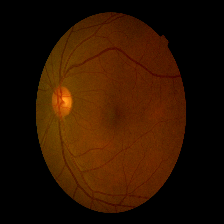
\includegraphics[width=0.188\textwidth]{fundus_grade0} &
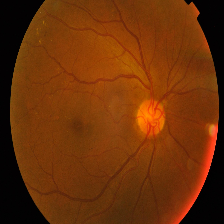
\includegraphics[width=0.188\textwidth]{fundus_grade1} &
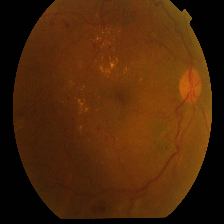
\includegraphics[width=0.188\textwidth]{fundus_grade2} &
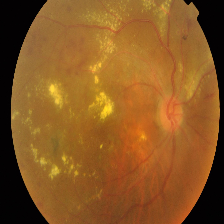
\includegraphics[width=0.188\textwidth]{fundus_grade3} &
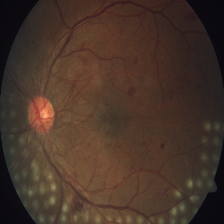
\includegraphics[width=0.188\textwidth]{fundus_grade4} \\[2pt]
\small\textbf{Grade 0} & \small\textbf{Grade 1} & \small\textbf{Grade 2} &
\small\textbf{Grade 3} & \small\textbf{Grade 4} \\
\footnotesize No DR & \footnotesize Mild NPDR & \footnotesize Moderate NPDR &
\footnotesize Severe NPDR & \footnotesize Proliferative DR
\end{tabular}
\caption[Representative fundus photographs for ICDR grades 0--4]{Representative fundus photographs for ICDR grades 0--4 (Kaggle EyePACS and
APTOS~2019 public datasets~\cite{kaggle2015eyepacs,aptos2019}). Lesion density and type
increase with grade: microaneurysms (Grade~1), haemorrhages and hard exudates (Grade~2),
venous beading and IRMA (Grade~3), neovascularisation (Grade~4).}
\label{fig:fundus}
\end{figure}

Grading is not an exact science. Even trained ophthalmologists disagree on a substantial
fraction of images, especially between adjacent grades, and the agreement depends on the
reference standard used: adjudication by a panel of retina specialists gives more
reliable labels than a single grader or a majority vote~\cite{krause2018grader}. Public
datasets are usually labelled by one or a few graders, so their labels contain some noise,
concentrated at the boundaries between grades. Any grading system, human or automated,
must therefore be judged against this intrinsic ambiguity. Many programmes grade each image
twice and send disagreements to a senior grader; an automated system is most useful when it
indicates which images deserve this second look. The calibrated probabilities and similar
reference cases of this thesis (\cref{ch:dots}) are first steps towards this role; an
automatic deferral of ambiguous images is left to future work. In the experiments of this thesis, the Mild--Moderate boundary concentrates the largest share of errors for every system (\cref{ch:toporet,ch:dots}), which is consistent with this intrinsic ambiguity.

\section{Screening Programmes and Patient Safety}
\label{sec:screening}

Population-scale screening is a public-health imperative, and automated
grading is widely seen as a way to make it more affordable at national
scale~\cite{ting2017jama,abramoff2018pivotal}. The safety of such a programme is measured by how many
sight-threatening cases it fails to refer. At a Severe-DR Non-Referral Rate of
$5.8\%$ -- the value of an EfficientNet-B3 baseline on the external Messidor-2 dataset in
this thesis -- a programme screening $500{,}000$ patients a year, of whom about $25{,}000$
have severe disease, would leave a projected $1{,}450$ severe cases unreferred every year (the assumptions of this
projection are stated in \cref{sec:impact}).

Organised screening has been shown to work at the scale of a country. In England, the
national programme started in 2003 invites every person with diabetes aged 12 and over for
annual photographic screening, with images graded in a multi-level quality-assured
process; since its introduction, diabetic retinopathy is no longer the leading cause of
certifiable blindness in the working-age population~\cite{scanlon2017english}. In the
United States, the EyePACS telemedicine network brought photographic screening to primary
care clinics by transmitting images to remote certified graders~\cite{cuadros2009eyepacs}
-- the same network that later provided the Kaggle dataset used in this thesis. Such
programmes need large numbers of trained graders, which is precisely the resource that
automated systems can save.

A screening programme is therefore judged on two different axes. Accuracy measures how
often the grade assigned to an image is correct, and is usually reported as the quadratic
weighted kappa (QWK) with the reference grader. Safety measures how often a patient who
needs urgent care is sent home, and is reported as the Severe-DR Non-Referral Rate
(Sev-NR). National programmes typically require a very low non-referral rate for
sight-threatening disease; this thesis adopts a target of $2\%$ throughout, used as a
predefined evaluation target rather than as a regulatory acceptance criterion. The two axes
do not move together: a system can gain several points of QWK while its Sev-NR stays above
the threshold, as the next section shows. The metrics are defined formally in
\cref{sec:metrics}.

\section{Public Datasets}
\label{sec:datasets}\label{app:datasets}

Research on automated DR grading relies on a small number of public datasets of colour
fundus photographs graded on the ICDR scale. Four of them are used in the DR experiments
of this thesis (\cref{tab:datasets}). Kaggle EyePACS~\cite{kaggle2015eyepacs} was released
for a public competition in 2015 and remains by far the largest. APTOS~2019~\cite{aptos2019}
was released for a second competition by an Indian tele-ophthalmology society.
Messidor-2~\cite{decenciere2014messidor} comes from French hospitals. KaggleDR-F1 is a
smaller Kaggle collection with five-grade labels, fused with APTOS~2019 in
\cref{ch:dots}. Other public datasets, such as IDRiD~\cite{porwal2018idrid,porwal2020idrid},
collected at a single Indian clinic with lesion segmentations, and DDR~\cite{li2019ddr},
from several Chinese hospitals, are also used in the literature; DRIVE~\cite{staal2004drive}
and STARE~\cite{hoover2000stare} provide manual vessel segmentations rather than grades and
have been central to the development of vessel segmentation methods.

\begin{table}[!htbp]
\centering
\caption[Grade distribution (\%) of the public datasets used in this thesis]{Grade distribution (\%) of the public datasets used in this thesis. Kaggle
EyePACS, APTOS~2019 and Messidor-2: counts distributed with the code of~\cite{belhadj2025plos}.}
\label{tab:datasets}
\small
\begin{tabular}{@{}lrccccc l@{}}
\toprule
Dataset & $N$ & G0 & G1 & G2 & G3 & G4 & Origin \\
\midrule
Kaggle EyePACS~\cite{kaggle2015eyepacs} & 35{,}126 & 73.5 & 7.0 & 15.1 & 2.5 & 2.0 & USA, multi-site \\
APTOS 2019~\cite{aptos2019} & 3{,}662 & 49.3 & 10.1 & 27.3 & 5.3 & 8.1 & India \\
Messidor-2~\cite{decenciere2014messidor} & 1{,}748 & 52.5 & 15.4 & 19.9 & 8.2 & 3.9 & France \\
KaggleDR-F1 & 2{,}197 & 49.3 & 10.1 & 27.3 & 5.3 & 8.1 & Kaggle collection \\
\bottomrule
\end{tabular}
\tabnote{$N$ counts retinal images, not independent patients: Kaggle EyePACS contains
both eyes of each patient. The full Kaggle EyePACS release has $88{,}702$ images; the
$35{,}126$ images with public labels are used in this thesis, as the TOPORET benchmark
(\enquote{Kaggle DR}) and as the external set of DGTS (\enquote{EyePACS}); $1{,}744$ of the $1{,}748$ Messidor-2 images are gradable.}
\end{table}

The datasets differ in ways relevant to the results of this thesis. Kaggle EyePACS, by
far the largest, aggregates images from many US clinical sites and camera models; it is
the most heterogeneous dataset and serves both as a TOPORET benchmark and as the external
validation set of DGTS. APTOS~2019 comes from an Indian screening programme. Messidor-2
(France, Topcon cameras) is a TOPORET benchmark and the external validation set of DOTS.
KaggleDR-F1 has exactly $60\%$ of the APTOS~2019 count in every grade, so its distribution
is identical to that of APTOS~2019; whether the two collections share images has not been
verified, a point discussed in \cref{ch:dots}. No dataset provides per-image demographic
annotations, so geographic diversity is only a proxy for population diversity. Grades~3
and~4 together are a minority in every dataset (from $4.5\%$ to $13.4\%$ combined), which
motivates class-balanced training: a system trained without correcting this imbalance would
under-predict exactly the two safety-critical grades on which Sev-NR and PDR-NR are
measured.

\section{Automated Grading: A Review of Methods}
\label{sec:decade}

Automated DR detection has been studied for more than two decades. Its history can be read
in four stages, which together explain the design of the systems developed in this
thesis. Recent reviews give a broader picture~\cite{tsiknakis2021review,alyoubi2020review,
ting2019ophthalmology}. The four stages are presented in chronological order, each with its main strength and the limitation that motivated the next one.

\subsection{Classical Image Analysis}

The first systems followed the reasoning of a human grader: detect the anatomical
landmarks, segment the vessels, find the lesions, and combine their counts into a
decision. Vessel segmentation received particular attention, with matched filters,
morphological operators and supervised pixel classifiers evaluated on the DRIVE and STARE
datasets~\cite{hoover2000stare,staal2004drive,fraz2012vessel}. Lesion detectors were
designed for bright lesions such as exudates~\cite{walter2002exudates} and for red lesions
such as microaneurysms and haemorrhages~\cite{niemeijer2005redlesions}. Combined into
complete systems, these methods reached screening-level sensitivity on large
populations~\cite{abramoff2008diabetes,abramoff2010retinal}. Their strength was
interpretability: every decision could be traced to detected lesions. Their weakness was
the accumulation of hand-tuned stages, each sensitive to image quality.

\subsection{Deep Convolutional Networks}

Deep learning replaced this pipeline by a single network trained end to end on graded
images~\cite{lecun2015deep,litjens2017survey}. In 2016, a convolutional network trained on
more than 100{,}000 graded images detected referable DR with a sensitivity and
specificity comparable to those of ophthalmologists~\cite{gulshan2016jama}, and similar
results were reported by other groups~\cite{abramoff2016improved,gargeya2017automated,
ting2017jama}. The Kaggle competition of 2015 popularised the quadratic weighted kappa as
the grading metric and led to many architectures based on standard ImageNet
backbones~\cite{he2016resnet,szegedy2016inception,tan2019efficientnet}. These networks
learn lesion detectors implicitly and are much more robust than hand-crafted pipelines,
but they are opaque, and their decisions are made one image at a time.

\subsection{Lesion-Aware and Attention Models}

A second generation of models tried to recover part of the interpretability of classical
systems. Lesion-mining approaches locate suspicious regions and use them to refine the
grade~\cite{quellec2017deep,wang2017zoomin}, while attention mechanisms weight the image
regions or the feature channels that matter most for each
grade~\cite{hu2018senet,he2021cabnet}. Systems trained on several tasks, such as lesion
segmentation and grading together, have extended detection to the whole disease spectrum,
including early stages~\cite{dai2021deepdr}. Visual explanations such as class activation
maps~\cite{zhou2016cam} or integrated gradients~\cite{sundararajan2017ig} have also been
shown to help human graders when displayed alongside the prediction~\cite{sayres2019integrated}.

\subsection{Transformers and Foundation Models}

Vision transformers~\cite{dosovitskiy2021vit} process an image as a sequence of patches
with self-attention, and capture long-range relations that convolutions see only
indirectly. Their main impact on DR grading has come through \emph{foundation models}:
networks pre-trained on very large unlabelled datasets and adapted to many tasks with
little labelled data~\cite{bommasani2021foundation}. RETFound~\cite{zhou2023retfound},
pre-trained by masked autoencoding on $1.6$ million retinal images, is the most prominent
example in ophthalmology and was reported to improve grading accuracy on several
benchmarks.

\subsection{Graph-Based and Population Approaches}

Graph neural networks, which learn on sets of related objects rather than isolated
samples, have been applied to many medical problems~\cite{ahmedt2021graphmed}. In
population graphs, each node is a patient and edges connect similar
patients~\cite{parisot2018disease}; the grade of a patient can then be informed by the
patients who resemble it. For DR, this line of work has remained limited to visual
similarity between images, and the global structure of the vessel network has not been
used to connect patients. \Cref{ch:background} introduces these methods in detail.

\subsection{Clinical Validation and Deployment}

Several systems have now been evaluated outside the laboratory. An autonomous system was
cleared by the US Food and Drug Administration in 2018 after a prospective trial in primary
care~\cite{abramoff2018pivotal}. Deep-learning systems were validated in national
programmes in India~\cite{gulshan2019india} and Thailand~\cite{ruamviboonsuk2019thailand},
and in a screening population in Zambia~\cite{bellemo2019zambia}. These studies confirm
that automated grading can match human graders on high-quality images, but they also
reveal practical obstacles: a study of a system deployed in Thai clinics found that
ungradable images, connectivity problems and workflow constraints reduced its usefulness
in practice~\cite{beede2020human}. More generally, the gap between retrospective accuracy
and clinical impact is now recognised as a central challenge of medical
AI~\cite{kelly2019challenges,liu2019comparison,rajpurkar2022ai}.

\subsection{Synthesis}

\Cref{tab:sota} summarises the systems most relevant to this thesis, from 2016 to 2026.
Accuracy has improved steadily, through better backbones, attention mechanisms and
retinal pre-training, but the three structural limitations defined in the next section
are not addressed together by any of the representative systems reviewed here.

\begin{table}[!htbp]
\centering
\caption[Comparison of DR grading systems, 2016--2026]{Comparison of DR grading systems,
2016--2026, with respect to the limitations L1--L3 of \cref{sec:limits}.}
\label{tab:sota}
\small
\setlength{\tabcolsep}{4pt}
\begin{tabular}{@{}l c P{5.2cm} c c c c@{}}
\toprule
System & Year & Key method & QWK & L1 & L2 & L3 \\
\midrule
Gulshan et al.~\cite{gulshan2016jama} & 2016 & Deep CNN (Inception-v3) & --$^{\dagger}$ & \xmark & \xmark & \xmark \\
CABNet~\cite{he2021cabnet} & 2021 & Category attention on a CNN backbone & --$^{\dagger}$ & \xmark & \xmark & \xmark \\
RETFound~\cite{zhou2023retfound} & 2023 & ViT-L/16, retinal pre-training & --$^{\dagger}$ & \xmark & \xmark & \xmark \\
SAMF-GB~\cite{belhadj2026samfgb}$^{\star}$ & 2026 & LightGBM $+$ structural features & 0.882 & \xmark & partial & \xmark \\
\midrule
TOPORET~\cite{belhadj2025plos}$^{\star}$ & 2026 & EfficientNet-B3 $+$ vessel TDA $+$ GraphSAGE & 0.88 & \cmark & \cmark & \xmark \\
DGTS~\cite{belhadj2026dgts}$^{\star}$ & 2026 & EfficientNet-B4 $+$ GraphSAGE $+$ PH regulariser & 0.941 & \cmark & partial & partial \\
DOTS~\cite{belhadj2026dots}$^{\star}$ & 2026 & EfficientNet-B3 $+$ FRE $+$ CORAL $+$ TTA & \textbf{0.953} & \xmark & \xmark & \cmark \\
\bottomrule
\end{tabular}
\tabnote{$^{\dagger}$Not reported in a form comparable to five-grade QWK (for example,
Gulshan et al.\ report AUC $=0.991$ for referable DR). $^{\star}$This thesis; QWK on the
dataset and protocol of the corresponding chapter (TOPORET: Kaggle DR, transductive five-fold cross-validation; DGTS and DOTS:
five-fold cross-validation on the fused APTOS~2019 $+$ KaggleDR-F1 corpus), not directly
comparable across rows. ``Partial'': DGTS uses feature-space rather than vascular topology,
and reports but does not meet the safety criterion on external data.}
\end{table}

Two patterns emerge from \cref{tab:sota}.

\paragraph{Pattern 1: accuracy gains do not resolve structural limitations.}
Better backbones and retinal pre-training improve accuracy, yet L1, L2 and L3 remain
unaddressed in each of the reviewed external systems. This suggests that the limitations
relate to architectural choices rather than to hyperparameters or dataset size, although
indirect mechanisms (for example global attention in transformers) may capture part of
the missing information.

\paragraph{Pattern 2: safety is rarely measured.}
None of the reviewed external systems reports the rate at which severe or proliferative
cases would be left unreferred under a five-grade protocol, and few are validated on a
dataset acquired in another country. A high QWK does not guarantee a low non-referral
rate: in \cref{ch:dots}, DGTS generalises well in QWK but its Sev-NR on external data
remains slightly above $2\%$.

\section{Challenges and Limits of Current Systems}
\label{sec:challenges}

Despite a decade of progress, automated DR grading still faces open challenges. Some are
practical: models trained on one population lose accuracy on images from other cameras or
other countries; public datasets are small for the severe grades; and a model that always
answers, even when the image is ambiguous, is hard to accept in a clinical workflow. This
thesis focuses on three limitations that are not practical but \emph{architectural}: they
recur across the representative systems reviewed above and are unlikely to be removed by
more data or larger networks alone. They are defined below as properties of an
architecture, so that each system of \cref{tab:sota} can be checked against them.

\subsection{Three Structural Limitations}
\label{sec:limits}

The following limitations are defined as binary architectural properties. They do not
depend on the volume of training data, on network depth or on computational budget.

\paragraph{Definition 1.1 (L1 -- No Relational Context).}
A system satisfies L1 if and only if $P(Y_i \mid I_i, \mathcal{C}) = P(Y_i \mid I_i)$,
where $\mathcal{C}$ denotes the patient cohort. All the per-image systems of
\cref{tab:sota} satisfy this condition.

\paragraph{Definition 1.2 (L2 -- No Vascular Topology).}
A system satisfies L2 if and only if its feature map $\varphi : I \to \mathbb{R}^d$ uses
only operations with bounded receptive fields (convolutions, local attention). Such a
map does not explicitly compute global topological invariants of the vascular network.

\paragraph{Definition 1.3 (L3 -- No Safety-Oriented Grading).}
A system satisfies L3 if and only if it is trained with an objective that ignores the
order of the grades and is evaluated without measuring the non-referral of severe and
proliferative cases against a safety threshold. Such a system cannot show that its errors
fall on the safe side of the referral decision.

\subsection{Why the Limitations Are Studied Together}
\label{sec:coupled}

A natural question is whether each limitation could be resolved by adding one component
to an existing system. The experiments of this thesis suggest that the answers interact.

Resolving \textbf{L1 alone} (adding a population graph built from visual similarity only,
as in DGTS) improves QWK by $0.018$ (\cref{tab:dgts-abl}), but leaves the topology of the
vessels unused; a dual metric that includes a topological distance requires the
topological pipeline of L2 to be already in place.

Resolving \textbf{L2 alone} (adding topological features without the graph) yields $+0.02$
QWK (\cref{tab:ablation3}) -- useful, but partial. The largest gain ($+0.04$ QWK) is
obtained only when topology is used both as a patient feature and inside the similarity of
the graph of L1, and the same complementarity is observed with DGTS under an inductive protocol
(\cref{ch:dots}).

Resolving \textbf{L3} requires more than an ordinal loss: on Messidor-2, CORAL alone leaves
Sev-NR at $3.7\%$, and only the complete DOTS pipeline reaches $1.4\%$ (\cref{tab:h3b}).
Conversely, DGTS improves accuracy and generalisation through L1 and L2 but does not meet
the safety threshold on external data.

\looseness=-1
This interaction is the motivating rationale for studying the three limitations in one
research programme (\cref{ch:toporet,ch:dots}). The thesis addresses them in complementary
systems; combining all three in one model is left to future work.

\subsection{Positioning of This Thesis}
\label{sec:position}

\Cref{tab:sota} makes the gap concrete: over a decade of progress in accuracy, none of the
representative external systems resolves the three structural limitations, because
per-image classifiers neither relate patients, nor compute global topological invariants,
nor target the referral decision (\cref{sec:limits}). This thesis therefore investigates
architectural additions rather than further scaling; \cref{tab:limits} summarises the three
limitations, their clinical consequence and the component that addresses each of them.

\begin{table}[!htbp]
\centering
\caption[The three structural limitations and how this thesis addresses them]{The three structural limitations and how this thesis addresses them.}
\label{tab:limits}
\footnotesize
\begin{tabular}{@{}P{3.0cm} P{4.6cm} P{5.6cm} c@{}}
\toprule
Limitation & Clinical consequence & Component of this thesis & Ch. \\
\midrule
L1 -- no relational context & Similar patients never inform each other's grade & Population graphs (TOPORET; inductive in DGTS) & 3--5 \\
L2 -- no vascular topology & Loss of vessel loops and rarefaction is not measured & Persistent homology of the vessel skeleton (TOPORET); topological regulariser (DGTS) & 3--5 \\
L3 -- no safety-oriented grading & Severe cases may be graded as No DR or Mild, unmeasured & CORAL ordinal head and safety evaluation with external validation (DOTS) & 5 \\
\bottomrule
\end{tabular}
\end{table}

\section*{Conclusion}
\phantomsection\addcontentsline{toc}{section}{Conclusion}

\looseness=-1
Despite a decade of gains in accuracy, the representative systems reviewed in this chapter
still grade each image in isolation (L1), ignore the topology of the vascular tree (L2) and
are rarely trained or evaluated with the referral of severe cases in mind (L3). Addressing
them requires learning on graphs, topological data analysis, ordinal prediction and
calibrated safety evaluation, which the next chapter introduces with the evaluation metrics.


\chapter{Learning on Graphs, Topology and Ordinal Prediction}
\label{ch:background}
\lofgroup{Chapter 2 -- Learning on Graphs, Topology and Ordinal Prediction}
\lotgroup{Chapter 2 -- Learning on Graphs, Topology and Ordinal Prediction}
\section*{Introduction}
\phantomsection\addcontentsline{toc}{section}{Introduction}

The previous chapter showed that current DR grading systems share three architectural
limitations: they ignore the relations between patients, they ignore the global
structure of the vascular tree, and they are rarely trained or evaluated with the
referral decision in mind. Each limitation calls for a family of methods that is well
established on its own but rarely used in medical image grading: graph neural networks for
relations between patients, topological data analysis for the structure of the vessels,
and ordinal prediction with calibrated probabilities for safety-oriented decisions.

This chapter introduces these methods and the tools used to evaluate them. We first
recall the deep-learning models used for medical images, from convolutional networks to
vision transformers and foundation models. We then present learning on graphs and the
inductive GraphSAGE model. Next, we introduce
persistent homology, which turns the shape of the vessel skeleton into numbers. We present
ordinal regression and the CORAL method, followed by uncertainty, calibration and
selective prediction, and by explainability. Finally, we define the evaluation metrics and
the statistical tests used in the experimental chapters.

\section{Deep Learning for Medical Image Analysis}
\label{sec:dl}

\subsection{Convolutional Neural Networks}

A convolutional neural network (CNN) processes an image through a stack of layers that
apply small learned filters over the whole image, followed by non-linearities and pooling
operations~\cite{lecun2015deep,goodfellow2016deep}. Early layers detect edges and textures,
deeper layers combine them into parts and objects. Because the same filter is applied at
every position, a CNN has far fewer parameters than a fully connected network and is
naturally robust to small translations, which suits images of lesions that can appear
anywhere on the retina.

The history of CNNs for image recognition is largely a history of depth. AlexNet showed in
2012 that a deep network trained on GPUs could outperform hand-crafted
features on ImageNet~\cite{krizhevsky2012imagenet,deng2009imagenet}. VGG networks stacked
small $3\times3$ filters~\cite{simonyan2015vgg}; Inception modules combined filters of
several sizes~\cite{szegedy2016inception}; residual networks made very deep models
trainable by adding shortcut connections~\cite{he2016resnet},
\begin{equation}
x_{l+1} = x_l + \mathcal{F}(x_l;\,W_l),
\label{eq:resnet}
\end{equation}
so that each block of \cref{eq:resnet} only learns a correction $\mathcal{F}$ to its input. DenseNet connected
every layer to all previous ones~\cite{huang2017densenet}, and EfficientNet scaled depth,
width and resolution together with a single coefficient~\cite{tan2019efficientnet}.
EfficientNet-B3 is the convolutional baseline used throughout this thesis. In medical
imaging, the same architectures, sometimes combined with segmentation networks such as
U-Net~\cite{ronneberger2015unet}, now dominate most tasks~\cite{litjens2017survey}, with
results that match specialists in dermatology~\cite{esteva2017dermatologist} and
ophthalmology~\cite{gulshan2016jama}.

\subsection{Attention and Vision Transformers}

Convolutions only look at a small neighbourhood at a time; relations between distant
regions of the image are captured indirectly, after many layers. The transformer
architecture~\cite{vaswani2017attention} replaces convolution by \emph{self-attention}, in
which every element of a sequence is updated with a weighted sum of all the others:
\begin{equation}
\mathrm{Attention}(Q,K,V) = \mathrm{softmax}\!\left(\frac{QK^\top}{\sqrt{d_k}}\right)V,
\label{eq:attention}
\end{equation}
where, in \cref{eq:attention}, the queries $Q$, keys $K$ and values $V$ are linear projections of the input. The
vision transformer (ViT)~\cite{dosovitskiy2021vit} applies this mechanism to an image cut
into patches of $16\times16$ pixels, each treated as a token. Transformers need more data
than CNNs to train from scratch, but scale better, and hierarchical variants such as the
Swin transformer~\cite{liu2021swin} bring back some of the locality of convolutions.
Attention weights are also used, with caution, as a form of explanation, since they show
which parts of the input the model relied on.

\subsection{Transfer Learning and Foundation Models}

Medical datasets are small compared with natural-image datasets, and labels are costly.
Transfer learning addresses this problem by initialising a model with weights learned on
another task, usually ImageNet classification, and fine-tuning it on the medical
task~\cite{pan2010transfer}. This practice is almost universal, although the features
learned on natural images are not always the most relevant for medical
images~\cite{raghu2019transfusion}.

Self-supervised learning removes the need for labels during pre-training: a network learns
by solving a task built from the data itself, such as recognising two augmented views of
the same image~\cite{chen2020simclr} or reconstructing masked image patches~\cite{he2022mae}.
Models pre-trained in this way on very large and diverse data, and then adapted to many
downstream tasks, are called \emph{foundation models}~\cite{bommasani2021foundation}.
RETFound~\cite{zhou2023retfound} is a vision transformer pre-trained with masked
autoencoding on $1.6$ million unlabelled retinal images. The systems of this thesis use
ImageNet-pre-trained EfficientNet backbones; replacing them by a retinal foundation model
is a direction for future work.

\subsection{Training Deep Networks}

Deep networks are trained by minimising a loss function with stochastic gradient descent
or one of its adaptive variants, of which Adam~\cite{kingma2015adam} is the most widely
used. Regularisation techniques such as dropout~\cite{srivastava2014dropout}, batch
normalisation~\cite{ioffe2015batchnorm} and data augmentation (random rotations, flips,
colour changes) reduce overfitting. For graded medical images, two further issues matter:
class imbalance, because severe grades are rare, and the ordinal nature of the labels.
Both are addressed in this thesis through the loss function (\cref{sec:coral}).

\section{Learning on Graphs}
\label{sec:graphs}

\subsection{Graphs and Message Passing}

A graph $G=(V,E)$ is a set of nodes $V$ connected by edges $E$. In a population graph,
each node is a patient (or a fundus image) described by a feature vector $x_v$, and an edge
between two nodes means that the two patients are similar. A graph neural network (GNN)
computes a representation $h_v$ of each node by repeatedly combining its own features with
those of its neighbours $\mathcal{N}(v)$. After $L$ rounds of this \emph{message passing},
the representation of a node summarises its $L$-hop neighbourhood, and a classifier
applied to $h_v$ can use information from similar patients to grade the current one.

Three architectures dominate the literature. The graph convolutional network
(GCN)~\cite{kipf2017gcn} averages neighbour features with fixed weights given by the graph
structure. The graph attention network (GAT)~\cite{velickovic2018gat} learns a weight
$\alpha_{ij}$ for each edge, so that the most informative neighbours count more. GraphSAGE,
presented below, samples a fixed number of neighbours and learns how to aggregate them.

Graph neural networks were first defined as recurrent models that propagate information
until a fixed point is reached~\cite{scarselli2009gnn}. Spectral approaches then defined
convolution on graphs through the eigenvectors of the graph
Laplacian~\cite{bruna2014spectral}, and fast polynomial approximations made them
practical~\cite{defferrard2016cheb}. Most current models can be written in the
\emph{message-passing} framework~\cite{gilmer2017mpnn,hamilton2020grl}, illustrated in
\cref{fig:mp}: at each layer, every node receives messages from its neighbours, aggregates
them, and updates its own representation.

% Figure 2.1 --- one round of message passing on a population graph
\begin{figure}[!htbp]
\centering
\resizebox{0.92\linewidth}{!}{%
\begin{tikzpicture}[
  font=\footnotesize,
  pt/.style={circle, draw=axisR, fill=axisRf, minimum size=7mm, inner sep=0},
  tg/.style={circle, draw=axisO, fill=axisOf, very thick, minimum size=8mm, inner sep=0},
  ed/.style={black!45, thick},
  msg/.style={-{Latex[length=2mm]}, axisR, very thick}
]
\begin{scope}
\node[tg] (v) at (0,0) {$v$};
\node[pt] (a) at (-1.6,1.1) {$u_1$};
\node[pt] (b) at (1.6,1.2) {$u_2$};
\node[pt] (c) at (-1.4,-1.3) {$u_3$};
\node[pt] (d) at (1.5,-1.2) {$u_4$};
\node[pt] (e) at (-3.0,0.1) {};
\node[pt] (g) at (3.0,0) {};
\foreach \x in {a,b,c,d} \draw[ed] (v) -- (\x);
\draw[ed] (a) -- (e); \draw[ed] (c) -- (e); \draw[ed] (b) -- (g); \draw[ed] (d) -- (g);
\node[below=12mm of v, align=center] {(a) patient $v$ and its neighbours\\in the population graph};
\end{scope}
\begin{scope}[xshift=7.2cm]
\node[tg] (v2) at (0,0) {$v$};
\node[pt] (a2) at (-1.6,1.1) {$u_1$};
\node[pt] (b2) at (1.6,1.2) {$u_2$};
\node[pt] (c2) at (-1.4,-1.3) {$u_3$};
\node[pt] (d2) at (1.5,-1.2) {$u_4$};
\foreach \x in {a2,b2,c2,d2} \draw[msg] (\x) -- (v2);
\node[draw=axisO, rounded corners=2pt, fill=white, align=center, font=\scriptsize] at (0,2.25)
  {$h_v^{(l)}=\sigma\bigl(W^{(l)}[\,h_v^{(l-1)}\,\Vert\,\mathrm{AGG}\{h_u^{(l-1)}\}\,]\bigr)$};
\node[below=12mm of v2, align=center] {(b) neighbours send their representations,\\which are aggregated and combined with $h_v$};
\end{scope}
\end{tikzpicture}}
\caption[One round of message passing on a population graph]{One round of message passing.
(a)~In a population graph, each node is a patient and edges connect similar patients.
(b)~Each neighbour sends its current representation; the messages are aggregated (for
example by a mean) and combined with the representation of $v$. After $L$ rounds, $h_v$
summarises the $L$-hop neighbourhood of the patient.}
\label{fig:mp}
\end{figure}


The choice of aggregation function determines what a GNN can distinguish: sum
aggregation is strictly more expressive than mean or max aggregation, as shown by the
graph isomorphism network (GIN)~\cite{xu2019gin}. Comprehensive surveys cover the many
variants proposed since~\cite{wu2021gnnsurvey,bronstein2017geometric}. In medicine, graphs
have been used to represent molecules, anatomical structures, brain connectivity and
populations of patients~\cite{ahmedt2021graphmed}. In a population graph, the edge
weights encode how similar two patients are, using image features or clinical
information~\cite{parisot2018disease}; the quality of this similarity is crucial, since a
graph that connects dissimilar patients propagates noise rather than signal.

\subsection{Inductive Inference with GraphSAGE}
\label{sec:sage}

GraphSAGE~\cite{hamilton2017graphsage} learns aggregation functions over sampled
neighbour sets:
\begin{align}
h^{(l)}_{\mathcal{N}(v)} &= \operatorname{MEAN}\bigl(\{\,h^{(l-1)}_u : u\in\mathcal{N}(v)\,\}\bigr),
\label{eq:sage-agg}\\
h^{(l)}_v &= \sigma\bigl(W^{(l)}\cdot\bigl[\,h^{(l-1)}_v \,\Vert\, h^{(l)}_{\mathcal{N}(v)}\,\bigr]\bigr).
\label{eq:sage-upd}
\end{align}
With $S=25$ samples per layer and $L=2$ layers, each prediction aggregates $S^L=625$
neighbour embeddings at $O(S^L)$ cost, independent of the size of the cohort. In a
$k$-nearest-neighbour graph with small $k$ (for example $k=8$ in DGTS, \cref{ch:dots}), a
node usually has fewer than $S$ neighbours, in which case all of them are used; $625$ is
therefore an upper bound. This inductiveness is a prerequisite for a screening service: a
new patient is graded by retrieving its neighbours from the reference index, without
retraining the graph (\cref{tab:latency}). GCN
in its original formulation~\cite{kipf2017gcn} is transductive and requires the full
graph at training time; GAT~\cite{velickovic2018gat} can be applied inductively (it was
evaluated on an inductive benchmark in the original paper), but it attends over complete
neighbourhoods, so its per-node cost grows with node degree (\cref{sec:gnnvariants}). For a screening service, where the population grows continuously, this difference is decisive: an inductive model can be deployed once and used for years, whereas a transductive one would have to be retrained whenever new patients join the graph.

\subsection{Choosing a Graph Architecture for Screening}
\label{sec:gnnvariants}

Three families of graph neural network were compared for clinical suitability.
\Cref{tab:gnn} compares their inference mode, per-patient cost, retraining need and
support for the per-prediction transparency required by Article~13 of the EU AI
Act~\cite{euaiact2024}.

\begin{table}[!htbp]
\centering
\caption[GNN variant comparison]{GNN variant comparison; inductive models with sampled
neighbourhoods suit a growing screening cohort. ``Art.~13'': support for per-prediction
transparency.}
\label{tab:gnn}
\small
\begin{tabular}{@{}lllP{3.3cm}c@{}}
\toprule
Model & Inference & Per-patient cost & Retraining for a new patient & Art.~13 \\
\midrule
GCN~\cite{kipf2017gcn} & Transductive & $O(|E|)$ per layer & Yes, full graph & Low \\
GAT~\cite{velickovic2018gat} & Inductive & $O(|\mathcal{N}(v)|)$ per layer & No & Medium \\
GraphSAGE~\cite{hamilton2017graphsage} & Inductive & $O(S^L)$, constant & No & Medium$^{\ast}$ \\
\bottomrule
\end{tabular}
\end{table}

Inductiveness is therefore a prerequisite for screening, which is why the graph-based
systems of this thesis use GraphSAGE. ($^{\ast}$) Although GraphSAGE has no attention
weights, the neighbours it aggregates are themselves an explanatory signal: DGTS returns
the retrieved similar cases with their verified grades (\cref{sec:audit}).

In practice, building a population graph requires three choices: the feature vector that
describes each patient, the similarity used to compare two patients, and the number $k$
of neighbours kept for each node. The first two decide which patients are considered
similar, and therefore what information the graph can propagate; the third controls a
trade-off between noise (too many weak neighbours) and isolation (too few). For cohorts of
tens of thousands of images, the $k$ nearest neighbours are found with approximate search
libraries such as FAISS~\cite{johnson2021faiss}, which keeps graph construction fast
enough for a screening service.

\section{Topological Data Analysis}
\label{sec:ph}

\subsection{From Vessel Skeletons to Point Clouds}

Topological data analysis (TDA) studies the \emph{shape} of data: how many connected
pieces it has, how many loops, and at which scale these features appear and disappear.
For retinal images, the object of interest is the vascular tree. After segmentation and
thinning, the vessels are reduced to a one-pixel skeleton, and the branch points of this
skeleton form a point cloud in the plane. Healthy vessels form a regular, tree-like
network; as DR progresses, capillaries close, abnormal shunts appear and new fragile vessels
grow, which changes the number of components and loops of the network.

\subsection{Simplicial Complexes and Homology}

Topology studies the properties of shapes that do not change under continuous
deformation, such as the number of connected pieces or of holes. To apply it to data, a
finite set of points must first be turned into a shape. A \emph{simplicial complex} does
this by gluing together simple building blocks: points (0-simplices), segments
(1-simplices), triangles (2-simplices) and their higher-dimensional
analogues~\cite{edelsbrunner2010computational}. The \emph{homology} of the complex then
counts its holes by dimension: the rank of $H_0$ is the number of connected components,
the rank of $H_1$ the number of independent loops (the first Betti number $\beta_1$), and
so on. For a vessel skeleton, $H_0$ reflects how fragmented the network is and $H_1$ how
many closed loops it contains.

\subsection{Persistent Homology}

For the branch points $P=\{p_1,\ldots,p_n\}$ of a vessel skeleton, the Vietoris--Rips
filtration adds a simplex $\sigma$ as soon as all pairwise distances within $\sigma$ are
at most $\varepsilon$. As $\varepsilon$ grows from $0$ to $\infty$, topological
features -- $H_0$ (connected components) and $H_1$ (independent loops) -- are born at scale
$b_j$ and die at $d_j$, with persistence $p_j=d_j-b_j$~\cite{edelsbrunner2002persistence,
carlsson2009topology}. The resulting persistence diagram $D$ summarises global structure
while being robust to local deformation: the stability
theorem~\cite{cohensteiner2007stability} bounds the change in the diagram by the change
in the filtering function,
\begin{equation}
d_B(D_f, D_g) \;\leq\; \lVert f-g\rVert_\infty ,
\label{eq:stability}
\end{equation}
where $d_B$ is the bottleneck distance. TOPORET compares diagrams with the closely related
Wasserstein distance $W_2$ (\cref{eq:dualsim}). This robustness makes the topological term of the
similarity less sensitive to small segmentation errors than a pixel-level comparison.

Persistence is what makes the method robust. A single threshold $\varepsilon$ would give
counts of components and loops that depend strongly on its value and on small errors of
segmentation; by following all thresholds at once, persistent homology keeps only the
features that survive over a wide range of scales. For a vessel skeleton, a short-lived
loop is typically an artefact of thinning, whereas a long-lived loop corresponds to a real
closed vascular circuit, such as an abnormal shunt or a neovascular frond.
\Cref{fig:filtration} illustrates the construction on a toy example. Persistent homology
was introduced as a way to separate robust topological features from
noise~\cite{edelsbrunner2002persistence,zomorodian2005computing}, and it is now the main
tool of topological data analysis~\cite{carlsson2009topology,chazal2021intro}.

% Figure 2.2 --- Vietoris--Rips filtration and persistence barcode on a toy point cloud
\begin{figure}[!htb]
\centering
\resizebox{\linewidth}{!}{%
\begin{tikzpicture}[font=\footnotesize]
\def\pts{(0,0),(1.2,0.1),(1.6,1.1),(0.8,1.8),(-0.2,1.1),(3.0,0.9)}
\foreach \k/\r/\lab in {0/0.08/{$\varepsilon=0$},1/0.62/{$\varepsilon_1$},2/0.8/{$\varepsilon_2$},3/1.05/{$\varepsilon_3$}}{
 \begin{scope}[xshift=\k*4.3cm]
  \foreach \p in \pts { \fill[axisSf, opacity=0.55] \p circle (\r); }
  \ifnum\k>0
   \draw[axisS, thick] (0,0)--(1.2,0.1)--(1.6,1.1)--(0.8,1.8)--(-0.2,1.1)--cycle;
  \fi
  \ifnum\k>2
   \fill[axisS, opacity=0.35] (0,0)--(1.2,0.1)--(1.6,1.1)--(0.8,1.8)--(-0.2,1.1)--cycle;
   \draw[axisS, thick] (1.6,1.1)--(3.0,0.9);
  \fi
  \foreach \p in \pts { \fill[black] \p circle (1.6pt); }
  \node at (1.4,-1.3) {\lab};
 \end{scope}}
% barcode
\begin{scope}[xshift=0cm, yshift=-4.6cm]
 \draw[-{Latex[length=2mm]}] (0,0) -- (16.5,0) node[right] {scale $\varepsilon$};
 \foreach \x/\l in {0/0, 4.3/{\varepsilon_1}, 8.6/{\varepsilon_2}, 12.9/{\varepsilon_3}} \draw (\x,0.08)--(\x,-0.08) node[below] {$\l$};
 \node[left] at (-0.2,1.55) {$H_0$};
 \foreach \y/\e in {1.1/4.3,1.3/4.3,1.5/4.3,1.7/4.3} \draw[axisR, line width=2pt] (0,\y) -- (\e,\y);
 \draw[axisR, line width=2pt] (0,1.9) -- (12.9,1.9);
 \draw[axisR, line width=2pt, -{Latex[length=2mm]}] (0,2.1) -- (16.3,2.1);
 \node[left] at (-0.2,0.55) {$H_1$};
 \draw[failred, line width=2.5pt] (4.3,0.55) -- (11.5,0.55);
 \node[right, font=\scriptsize, text=failred] at (11.6,0.55) {one persistent loop};
\end{scope}
\end{tikzpicture}}
\caption[Vietoris--Rips filtration and persistence barcode]{Vietoris--Rips filtration on a
toy point cloud of six points and the resulting barcode. As the scale $\varepsilon$ grows,
balls around the points merge: components ($H_0$ bars) die when they join, a loop ($H_1$
bar, red) is born when the five points on the left close a cycle and dies when the cycle is
filled. Long bars correspond to robust structure, short bars to noise. In this thesis the
points are the branch points of the vessel skeleton.}
\label{fig:filtration}
\end{figure}


\subsection{From Diagrams to Features}

A persistence diagram is a set of points of variable size, which cannot be fed directly to
a standard learning model. Several vector representations have been proposed: persistence
landscapes~\cite{bubenik2015landscapes}, persistence images~\cite{adams2017images}, learned
layers that process diagrams inside a neural
network~\cite{hofer2017topological,carriere2020perslay}, and simple summary statistics such
as total persistence, number of features or the longest bar. Efficient software makes these
computations practical on large datasets~\cite{otter2017roadmap,maria2014gudhi,
tauzin2021giotto}. This thesis uses a small vector of interpretable summary statistics
(\cref{eq:tda}), which can be related directly to vascular pathology.

\section{Ordinal Prediction}
\label{sec:coral}

\subsection{Why DR Grading Is an Ordinal Problem}

The five ICDR grades are ordered: Grade~3 is worse than Grade~2, which is worse than
Grade~1. A standard classifier ignores this order and treats a confusion between Grade~0
and Grade~4 exactly like a confusion between Grade~3 and Grade~4, although the first is a
serious clinical error and the second is a disagreement that also occurs between experts.
Ordinal regression methods decompose the problem into $K-1$ binary questions of the form
``is the grade at least $k$?'' and combine their answers.

\subsection{Families of Ordinal Methods}

Ordinal regression has a long history in statistics and machine
learning~\cite{gutierrez2016ordinal}. A simple and general approach transforms a
$K$-class ordinal problem into $K-1$ binary problems, ``is the grade greater than $k$?'',
and combines their probabilities~\cite{frank2001ordinal}. Deep versions of this idea train
a network with $K-1$ binary outputs~\cite{niu2016ordinal}, but nothing guarantees that the
estimated probabilities decrease with $k$, so the model can produce inconsistent rankings.
Other works keep a standard classifier and change the loss, for example by directly
optimising the weighted kappa~\cite{delatorre2018kappa}. CORAL and CORN, presented next,
are the two most widely used deep ordinal methods with a rank-consistency property.

\subsection{CORAL and CORN}

CORAL~\cite{cao2020coral} obtains rank consistency from the architecture rather than from
a loss penalty. All $K-1$ binary tasks share the same weight vector $w\in\mathbb{R}^d$ and
differ only by their biases $b_1,\ldots,b_{K-1}$, so that
$\hat P(Y\geq k)=\sigma(w^{\top}h+b_k)$. Cao et al.\ show that the biases minimising the
CORAL loss are ordered, $b_1\geq\cdots\geq b_{K-1}$; the ordering can also be enforced
explicitly during training by the projection
\begin{equation}
b_k \leftarrow \min(b_k,\, b_{k-1} - \epsilon), \qquad k=2,\ldots,K-1 .
\label{eq:coral-proj}
\end{equation}
With ordered biases, $\hat P(Y\geq 1)\geq \hat P(Y\geq 2)\geq\cdots$ holds for every input:
the cumulative probabilities cannot cross. CORN~\cite{shi2023corn} obtains rank
consistency differently: its $K-1$ binary tasks estimate conditional probabilities
$\hat P(Y>k\mid Y>k-1)$, and the cumulative probabilities are their chain-rule product,
which cannot increase with $k$ provided the outputs are decoded in this way.

\Cref{fig:coral} summarises the resulting architecture. The single shared weight vector
is what makes the guarantee possible: all binary questions use the same score $s_i$, and
only the thresholds $b_k$ move along it.

% CORAL head schematic
\begin{figure}[!tb]
\centering
\resizebox{0.95\linewidth}{!}{%
\begin{tikzpicture}[font=\footnotesize,
  box/.style={draw, rounded corners=2pt, align=center, inner sep=3pt, minimum height=0.75cm},
  arr/.style={-{Latex[length=2mm]}, thick}]
\node[box, fill=black!6, draw=black!55, minimum height=3.8cm, minimum width=1.7cm] (z) at (0,0) {Embedding\\$z_i$};
\node[box, fill=axisRf, draw=axisR, minimum height=3.8cm, minimum width=2.2cm] (w) at (3.2,0) {Shared\\weights $w$\\[4pt]$s_i = w^\top z_i$};
\node[font=\bfseries\scriptsize] at (6.9,2.35) {Logits};
\node[font=\bfseries\scriptsize] at (10.3,2.35) {$\hat P(Y\geq k)$};
\foreach \k/\y in {1/1.35,2/0.45,3/-0.45,4/-1.35}{
  \node[box, fill=axisOf, draw=axisO, minimum width=2.4cm] (g\k) at (6.9,\y) {$g_i^{(\k)} = s_i + b_\k$};
  \node[box, fill=white, draw=black!55, minimum width=2.2cm] (p\k) at (10.3,\y) {$\sigma\big(g_i^{(\k)}\big)$};
  \draw[arr] (w.east) -- (g\k.west);
  \draw[arr] (g\k) -- (p\k);
}
\draw[arr] (z) -- (w);
\node[box, fill=okf, draw=okgreen, minimum height=3.8cm, minimum width=3.2cm] (y) at (14.2,0) {Grade $\hat y_i$\\[4pt]number of $k$\\with $\hat P(Y\geq k)>0.5$};
\foreach \k in {1,2,3,4} \draw[arr] (p\k.east) -- (y.west |- p\k.east);
\node[font=\scriptsize, text=axisO, align=center] at (6.9,-2.55) {$b_1\geq b_2\geq b_3\geq b_4$\\enforced after each update};
\node[font=\scriptsize, align=center] at (10.3,-2.55) {decreasing in $k$\\$\Rightarrow 0$ rank violations};
\end{tikzpicture}}
\caption[The CORAL ordinal head]{The CORAL ordinal head. A single weight vector $w$ is shared
by the $K-1=4$ binary questions ``is the grade at least $k$?''; only the biases $b_k$ differ.
Because the biases are kept ordered, the estimated probabilities always decrease with $k$,
whatever the input and the weights, and the grade is simply the number of questions
answered ``yes''.}
\label{fig:coral}
\end{figure}


Rank consistency matters beyond elegance. A model that gives a higher probability to
``at least Grade~4'' than to ``at least Grade~3'' produces an output that has no clinical
meaning and cannot be explained to a grader. It also makes the choice of a referral rule
ambiguous, since different thresholds on the cumulative probabilities can lead to
contradictory decisions. With CORAL, the cumulative probabilities form a proper survival
function over the grades, and the grade is decoded by counting the binary tasks whose
probability exceeds $0.5$, $\hat y=\sum_k\mathbb{1}[\hat P(Y\geq k)>0.5]$; this is the
decoding used by DOTS (\cref{ch:dots}).

\section{Uncertainty, Calibration and Selective Prediction}
\label{sec:calib}

\subsection{Calibration}

The Expected Calibration Error (ECE)~\cite{naeini2015ece,guo2017calibration} partitions the $n$
predictions into $M$ confidence bins $B_m$ and measures the gap between accuracy and
confidence:
\begin{equation}
\mathrm{ECE} = \sum_{m=1}^{M} \frac{|B_m|}{n}\,\bigl|\operatorname{acc}(B_m) - \operatorname{conf}(B_m)\bigr| .
\label{eq:ece}
\end{equation}
An ECE of $0.031$, the value reached by DOTS after temperature scaling (\cref{ch:dots}),
means that on average its predicted confidence departs from empirical accuracy by about
$3$ percentage points. Temperature scaling~\cite{guo2017calibration} divides the logits
by a single scalar $T$ fitted on validation data, which changes the confidence but not the
predicted grade.

\subsection{Sources of Uncertainty}

The uncertainty of a prediction has two sources~\cite{kendall2017uncertainties}.
\emph{Aleatoric} uncertainty comes from the data itself: an image may be blurred, or the
lesions may be genuinely at the boundary between two grades, and more training data will
not remove this ambiguity. \emph{Epistemic} uncertainty comes from the model: it is high
for inputs unlike those seen during training, and decreases with more data. Estimating
epistemic uncertainty usually requires several predictions per input, obtained with Monte
Carlo dropout~\cite{gal2016dropout} or with an ensemble of independently trained
networks~\cite{lakshminarayanan2017ensembles}. In medical decision making, reporting
uncertainty is increasingly seen as a requirement rather than an
option~\cite{begoli2019uncertainty}. The systems of this thesis report calibrated
single-pass probabilities; ensemble or Monte Carlo estimates of epistemic uncertainty are
not used.

\subsection{Selective Prediction and Abstention}

The idea of letting a classifier reject uncertain inputs is old: Chow showed in 1970
that, for a given cost of errors and of rejections, the optimal rule rejects the inputs
whose highest class probability is below a threshold~\cite{chow1970reject}. A calibrated model knows, to some extent, when it is likely to be wrong. Selective
prediction uses this information to let the model \emph{abstain}: when the uncertainty of a
prediction exceeds a threshold, the case is deferred to a human expert instead of being
graded automatically~\cite{geifman2017selective}. Two quantities then describe the system:
the \emph{coverage}, i.e.\ the fraction of cases graded automatically, and the error rate on
the cases that are graded. Lowering the threshold defers more cases and reduces errors, at
the cost of more work for human graders. Selective prediction is not implemented in the
systems of this thesis; building it on the calibrated probabilities of DOTS is one of the
perspectives of the General Conclusion.

\section{Explainability}
\label{sec:xai}

A clinician who receives an automated grade needs to know why it was given, and European
regulation requires that high-risk AI systems be transparent to their users. Explanation
methods for image classifiers fall into two groups. \emph{Post-hoc} methods explain a
trained model from outside: class activation maps~\cite{zhou2016cam} and
Grad-CAM~\cite{selvaraju2017gradcam} highlight the image regions that most influenced the
decision, integrated gradients~\cite{sundararajan2017ig} attribute the prediction to input
pixels, and model-agnostic methods such as LIME~\cite{ribeiro2016lime} and
SHAP~\cite{lundberg2017shap} approximate the model locally with a simple one. For DR,
displaying such explanations has been shown to help graders~\cite{sayres2019integrated}.
Their limitation is that they approximate the model and may not reflect its actual
reasoning. \emph{Intrinsic} explanations, by contrast, come from quantities that the model
computes to make its decision, such as attention weights or interpretable features.
Intrinsic signals are not automatically faithful either: attention weights, in
particular, are not guaranteed to measure the causal importance of each input. The
systems of this thesis rely on such intrinsic explanatory signals -- the similar
patients retrieved by the graph with their verified grades, the topological features of
the vessel network and calibrated probabilities (\cref{sec:audit}) -- whose faithfulness was
not evaluated in this thesis.

\section{Evaluation Metrics and Statistical Tests}
\label{sec:metrics}

\subsection{Metrics}

The following metrics are used throughout the experimental chapters.
\begin{description}[style=nextline,leftmargin=1.2em]
\item[Quadratic weighted kappa (QWK)] Agreement between predicted and reference grades,
corrected for chance and weighted by the squared distance between grades:
\begin{equation}
\kappa_w = 1-\frac{\sum_{i,j} w_{ij}\,O_{ij}}{\sum_{i,j} w_{ij}\,E_{ij}},\qquad
w_{ij}=\frac{(i-j)^2}{(K-1)^2},
\label{eq:qwk}
\end{equation}
where, in \cref{eq:qwk}, $O$ is the observed confusion matrix and $E$ the matrix expected by
chance~\cite{cohen1968weighted}. QWK is the standard accuracy metric of DR grading
challenges.
\item[Area under the ROC curve (AUC)] Ability to separate referable from non-referable
images, independently of the decision threshold~\cite{hanley1982auc}.
\item[Expected calibration error (ECE)] Gap between confidence and accuracy
(\cref{eq:ece}).
\item[Severe-DR non-referral rate (Sev-NR)] Fraction of Grade~3 images predicted as No DR
or Mild, grades that do not trigger referral (\cref{eq:nr}). It is the primary safety
metric of this thesis, with a threshold of $2\%$.
\item[PDR non-referral rate (PDR-NR)] The same quantity for Grade~4.
\item[Rank violations] Fraction of predictions for which the cumulative probabilities
$\hat P(Y\geq k)$ are not decreasing in $k$.
\end{description}

\subsection{Statistical Tests}

Each hypothesis of the thesis is tested with an explicit statistical procedure. A paired
$t$-test compares two systems evaluated on the same cross-validation folds. A one-way
analysis of variance (ANOVA), followed by Tukey's post-hoc test~\cite{tukey1949}, tests
whether a feature differs across the five grades. Wilcoxon and McNemar tests compare paired
folds or paired predictions. Bootstrap resampling~\cite{efron1993bootstrap} gives
confidence intervals for QWK, and exact Clopper--Pearson intervals are used for the
non-referral rates, which are proportions of small counts. Effect sizes are reported with Cohen's $d$ and $\eta^2$~\cite{cohen1988}. The
formal statements are collected in \cref{app:stats}.

\section{Summary of the Methods}
\label{sec:methods-summary}

\Cref{tab:methods} summarises where each method introduced in this chapter is used in the
rest of the thesis and which limitation it addresses.

Two observations follow from \cref{tab:methods}. First, each limitation is addressed by a
method with a formal property rather than by a heuristic: inductiveness for the graph,
stability for persistence diagrams, rank consistency for CORAL and calibration for the
confidence scores. Second, the methods are complementary rather than redundant: the graph
and the topology act on the representation of a patient, whereas the ordinal head and
calibration act on the decision taken from that representation. The experimental chapters
test whether this complementarity holds in practice.

\begin{table}[!htbp]
\centering
\caption{Methods introduced in this chapter and their role in the thesis.}
\label{tab:methods}
\small
\begin{tabular}{@{}P{4.2cm} P{6.2cm} c c@{}}
\toprule
Method & Role in the thesis & Limitation & Chapters \\
\midrule
EfficientNet-B3/B4 & Visual features of the fundus image & -- & 3--5 \\
GraphSAGE & Inductive population graph; grading of a new patient without retraining & L1 & 3--5 \\
Persistent homology & Descriptors of the vessel skeleton (TOPORET) and of feature-space neighbourhoods (DGTS) & L2 & 3--5 \\
CORAL & Rank-consistent ordinal head of DOTS & L3 & 5 \\
Temperature scaling & Calibrated confidence scores & L3 & 5 \\
QWK, AUC, ECE, Sev-NR & Accuracy, calibration and safety evaluation & -- & 3--5 \\
\bottomrule
\end{tabular}
\end{table}

\section*{Conclusion}
\phantomsection\addcontentsline{toc}{section}{Conclusion}

This chapter introduced the tools of the thesis: convolutional features, the inductive
GraphSAGE model, persistent homology of the vessel skeleton, CORAL ordinal regression and
temperature scaling, together with metrics that separate accuracy, calibration and safety.
The next chapter tests these tools on simpler settings before applying them to the retina.


\chapter{Structural and Topological Priors for Retinal Image Grading}
\label{ch:found}
\lofgroup{Chapter 3 -- Structural and Topological Priors for Retinal Image Grading}
\lotgroup{Chapter 3 -- Structural and Topological Priors for Retinal Image Grading}
\section*{Introduction}
\phantomsection\addcontentsline{toc}{section}{Introduction}

Before building a complete grading system, two questions must be answered. First, does
the GraphSAGE template with structural descriptors behave as a general architectural
property, or does it only work on one particular dataset? Second, do global structural and
topological features of the retina actually carry information that a deep network trained
on the raw image does not already capture? If either answer were negative, the systems of
the following chapters would rest on weak foundations.

This chapter answers both questions with the first contributions of the thesis. In
Part~A, we validate the graph template on distributed-systems data, where graphs are
natural and ground truth is unambiguous: microservice orchestration and anomaly detection
on six benchmarks. We then explain how each element of this template is transferred to
retinal grading. In Part~B, we move to diabetic retinopathy and test the value of
structural features with three independent methods: a hybrid CNN--GNN model with
topological features, a gradient-boosting model on hand-crafted structural features
(SAMF-GB), and a reduced CPU-efficient variant (LightGBM-HC). Weaker intermediate results
are reported deliberately, to show how the final solution was built step by step.

\section{Part A: Validating the Graph Template Outside Medicine}
\label{sec:ch2-rationale}

Part~A validates the GraphSAGE architectural template on six structurally diverse,
non-medical benchmarks before any contact with retinal images. The rationale is
epistemological: if the structural-invariant augmentation works across six domains with
very different graph topologies, the expectation that it will transfer to inter-patient
similarity graphs rests on reproducible evidence rather than on analogy alone. This
six-benchmark validation is Contribution~C1; it also makes the architectural choices of
TOPORET and DOTS easier to defend before a regulatory reviewer.

\paragraph{Why distributed systems?}
Validating a graph architecture requires data where the graph is natural and the labels
are unambiguous. Microservice architectures and computer networks provide exactly this:
the dependencies between services or hosts form an explicit graph, and failures or attacks
are recorded without the inter-grader disagreement that affects medical labels. They also
share an essential property with a screening service: the system must make decisions on
new nodes as they appear, without being retrained. A template that works in these
conditions is a credible candidate for a population graph of patients, and any weakness
found there can be corrected before touching medical data.

\subsection{GNN-MSOrchest: Microservice Cascade-Failure Recovery}
\label{sec:msorchest}

GNN-MSOrchest~\cite{belhadj2025icaart} models a 48-service e-commerce microservice system
as a directed attributed graph $G=(V,E,X)$. Each node $v\in V$ carries a five-dimensional
health vector $x_v=[\mathrm{CPU},\mathrm{mem},\mathrm{lat},\mathrm{err},\mathrm{dep}]^\top$
updated every $200$~ms. Edges encode directed dependencies (service $u$ calls service
$v$) with propagation-delay attributes. A two-layer GraphSAGE with mean aggregation drives
adaptive workload allocation:
\begin{equation}
\hat y_v = \mathrm{MLP}\bigl(h^{(2)}_v\bigr),
\label{eq:msorch}
\end{equation}
where $h^{(2)}_v$ is the node representation after two message-passing rounds with
$d_h=256$ and $S=25$ sampled neighbours per layer. The prediction $\hat y_v$ of \cref{eq:msorch} drives
load-shedding decisions for node $v$ during cascade propagation.

\paragraph{Structural-invariant augmentation.}
The key methodological contribution is the augmentation
$h_{\mathrm{aug}}=[\,h_{\mathrm{GNN}}\,\Vert\,I(v)\,]$, where $I(v)$ is a
four-dimensional structural descriptor:
\begin{equation}
I(v) = \bigl(\delta(v),\, c(v),\, b(v),\, h(v)\bigr)^\top ,
\label{eq:invariants}
\end{equation}
with $\delta(v)$ the degree centrality, $c(v)$ the clustering coefficient, $b(v)$ the
betweenness centrality and $h(v)$ the local structural entropy. These quantities depend
only on graph topology, not on node features or learned representations, and are cheap
to compute (linear in $|V|+|E|$ for all but betweenness, which is approximated by
sampling).

\Cref{tab:msorch} compares GNN-MSOrchest with a static-threshold baseline. The cascade
isolation mechanism -- withholding load from nodes whose predictive entropy exceeds a
threshold -- is the direct methodological precursor of the entropy abstention of DOTS
(\cref{sec:abst}).

\begin{table}[H]
\centering
\caption[GNN-MSOrchest versus a static-threshold baseline]{GNN-MSOrchest versus a static-threshold baseline (SimPy simulation, 48
nodes)~\cite{belhadj2025icaart}.}
\label{tab:msorch}
\small
\begin{tabular}{@{}lcc@{}}
\toprule
Metric & Static-threshold baseline & GNN-MSOrchest \\
\midrule
Mean response time (ms) & 142 & 98 ($-31.0\%$) \\
p99 latency (ms) & 510 & 287 ($-43.7\%$) \\
Cascade-failure containment & 34\% & 81\% ($+47$~pp) \\
Resource-utilisation Gini coefficient & 0.41 & 0.18 ($-56.1\%$) \\
\bottomrule
\end{tabular}
\end{table}

\subsection{Structural Invariants Across Six Benchmarks}
\label{sec:invariants}

The second publication~\cite{belhadj2026invariants} tests whether the augmentation of
\cref{eq:invariants} gives statistically significant and stable gains across six
benchmarks with heterogeneous graph structure: a synthetic controlled graph, two
network-intrusion datasets (KDD Cup~1999~\cite{tavallaee2009nslkdd},
CICIDS~2017~\cite{sharafaldin2018cicids}), a more recent network-intrusion
dataset (UNSW-NB15~\cite{moustafa2015unsw}), a refined intrusion benchmark
(NSL-KDD~\cite{tavallaee2009nslkdd}) and a production
microservice trace (SockShop/Istio).

\Cref{tab:invariants} reports the six results. Each row is one benchmark: its domain,
the F1 score of the plain GNN, the F1 score once the four invariants $I(v)$ are appended
to the node features, and the resulting gain in recall on the anomalous class. The recall
gain is positive on every benchmark and lies between $+3.1$ and $+5.0$~pp (mean $+4.2$~pp, standard deviation $0.6$~pp). The
coefficient of variation ($0.6/4.2\approx 14\%$) is low, so the effect is stable across
domains rather than driven by a single benchmark.

\begin{table}[H]
\centering
\caption[Structural-invariant augmentation across six graph benchmarks]{Structural-invariant augmentation across six graph
benchmarks~\cite{belhadj2026invariants}.}
\label{tab:invariants}
\small
\begin{tabular}{@{}llccc@{}}
\toprule
Benchmark & Domain & F1 (GNN) & F1 ($+I(v)$) & $\Delta$ recall \\
\midrule
Synthetic graph & Controlled network & 85.3\% & 93.5\% & $+5.0$~pp \\
KDD Cup 1999 & Network intrusion (classic) & 88.1\% & 94.2\% & $+4.6$~pp \\
CICIDS 2017 & Multi-protocol IDS & 86.7\% & 92.0\% & $+4.1$~pp \\
UNSW-NB15 & Network intrusion (recent) & 84.9\% & 90.8\% & $+3.1$~pp \\
NSL-KDD & Intrusion (refined) & 87.4\% & 93.1\% & $+4.4$~pp \\
SockShop/Istio & Production microservices & 89.2\% & 95.3\% & $+4.4$~pp \\
\midrule
Mean (SD) & & 87.0\% (1.5) & 93.2\% (1.6) & $+4.2$~pp (0.6) \\
\bottomrule
\end{tabular}
\end{table}

\subsection{Transfer Architecture and Its Justification}
\label{sec:transfer}

The transfer from distributed systems to DR grading is direct at the level of the
architecture: GraphSAGE with $L=2$, $d_h=256$, dropout $p=0.30$, Adam with learning rate
$10^{-3}$ and $S=25$ is used unchanged. The structural augmentation
$h_{\mathrm{aug}}=[\,h_{\mathrm{GNN}}\Vert I(v)\,]$ becomes
$z_i=[\,x_i^{\mathrm{CNN}}\Vert x_i^{\mathrm{TDA}}\,]$, and the cascade isolation of
uncertain nodes becomes entropy abstention at threshold $\tau_U$.

\paragraph{From distributed systems to retinal grading.}
The transfer rests on a one-to-one correspondence between the objects of the two
domains, set out in \cref{tab:mapping} in pipeline order. The first three rows define the
nodes and what they carry: a service becomes a patient, the service health vector
becomes the CNN embedding of the fundus image, and the structural invariant $I(v)$
becomes the topological feature vector of \cref{eq:tda}. The fourth row defines the
edges: a dependency between services becomes a dual-similarity edge between patients
(\cref{eq:dualsim}). The last three rows define behaviour: a cascade failure becomes
diagnostic uncertainty spreading across a grade boundary, load shedding becomes
abstention, and recall-prioritised anomaly detection becomes the class-weighted CORAL
loss that favours the rare severe grades. Read row by row, the table is a checklist:
every component validated on network graphs has a named counterpart in TOPORET
(\cref{ch:toporet}) and DOTS (\cref{ch:dots}).

\begin{table}[H]
\centering
\caption[Mapping from distributed-systems concepts to DR-grading analogues]{Conceptual mapping from distributed-systems concepts (this chapter) to their
DR-grading analogues (\cref{ch:toporet,ch:dots}).}
\label{tab:mapping}
\small
\begin{tabular}{@{}P{6.4cm}P{8.0cm}@{}}
\toprule
Distributed-systems concept & DR-grading analogue \\
\midrule
Service node $v\in V$ & Patient $i$ \\
Service health vector (CPU, memory, latency, \ldots) & CNN embedding $x_i^{\mathrm{CNN}}$ \\
Structural invariant $I(v)$ (degree, clustering, betweenness, entropy) & Topological feature vector $x_i^{\mathrm{TDA}}$ (\cref{eq:tda}) \\
Dependency edge (service $u$ calls service $v$) & Population-graph edge (dual similarity $S_{ij}$, \cref{eq:dualsim}) \\
Cascade failure (overload propagating across services) & Diagnostic uncertainty propagating across a grade boundary \\
Load-shedding decision (withhold traffic from an overloaded node) & Abstention (defer to a specialist when $H_i>\tau_U$) \\
Recall-prioritised anomaly detection (rare-event sensitivity) & Class-weighted CORAL loss ($\lambda_3=8$, $\lambda_4=6$) \\
\bottomrule
\end{tabular}
\end{table}

\paragraph{Why hyperparameters transfer without re-tuning.}
A natural objection is that hyperparameters validated on network-traffic and microservice
graphs may not suit a population graph of patients. Two considerations mitigate this.
First, the graphs of Part~A already span a wide range of sizes (from the 48-node SimPy
testbed of \cref{tab:msorch} to the traffic graphs of \cref{tab:invariants}, with several
thousand nodes) and densities, and the augmentation gain of \cref{tab:invariants} is stable
across the six benchmarks. Second, the population
graphs of \cref{ch:toporet,ch:dots} (several thousand to tens of thousands of nodes,
$k=15$ neighbours per node) fall within that range, so the transfer is an interpolation
rather than an extrapolation. The hyperparameter sensitivity analysis was nevertheless
repeated on DR data (\cref{tab:hparam}) as a confirmatory check.

\paragraph{What the transfer claims and does not claim.}
The transfer is architectural, not distributional. It does not claim that retinal
population graphs and microservice graphs share statistical properties, nor that
performance on one guarantees performance on the other. It claims that the same
architectural pattern -- GraphSAGE with mean aggregation, $L=2$ hops, $d_h=256$,
structural-invariant augmentation -- transfers without modification, which is evidence
for the genericity of the approach. The cross-domain validation is methodological
insurance, not a proof of universal applicability.

\subsection{Threats to the Transfer Argument}
\label{sec:threats}

Three threats deserve to be named. First, all six benchmarks are graphs over discrete
events or entities (network flows, service calls); a population graph over patients
carries node features of a different statistical character, and stability across event
graphs does not by itself guarantee stability across patient-similarity graphs. Second,
the benchmarks share an implicit assumption that better-connected neighbourhoods are more
informative. Its analogue for disease severity -- that similar patients share diagnostic
information -- is precisely what H1 tests, not a premise this chapter can establish.
Third, six benchmarks remain a finite, non-random sample of graph domains; the
coefficient-of-variation argument supports stability within this sample only.

These caveats do not undermine the strategy; they are why the hyperparameter analysis is
repeated on retinal data (\cref{sec:dualsim}) instead of relying on Part~A alone.

\section{Part B: Structural Evidence on Retinal Data}
\label{sec:partb}

Part~B presents three convergent proof-of-concept validations of the structural axis
(the answer to L2). Three methodologies -- a deep hybrid model, gradient boosting with SHAP attribution, and
a leave-one-family-out ablation -- each indicate that global structural priors improve DR
grading.
This convergence motivates the formal statistical test of H2 in \cref{ch:toporet}.

\paragraph{Experimental setting.}
The three studies of Part~B use the public datasets of \cref{sec:datasets}. The hybrid
CNN--GNN model was developed on APTOS~2019 with a binary target (No DR versus any DR),
which allowed many ablation runs at low cost. SAMF-GB and LightGBM-HC were evaluated on the
five-grade task on Kaggle EyePACS, the benchmark used for TOPORET and DOTS in the following
chapters, with five-fold cross-validation stratified by grade. SAMF-GB and LightGBM-HC
extract the vessel network with the same pre-processing (CLAHE and Zhang--Suen
skeletonisation); the hybrid model instead computes its descriptors from
structure-enhanced intensity responses, without explicit vessel segmentation. The three
studies therefore differ in data, task and input representation, and their results are
compared qualitatively rather than numerically.

\subsection{Hybrid CNN--GNN with Geometric and Topological Invariants}
\label{sec:hybrid}

The first retinal study~\cite{belhadj2026hybrid}, extended in the book
chapter~\cite{mezghich2026lnaitopo}, tests whether global structural descriptors add
information to a deep CNN--GNN pipeline. An EfficientNet-B0 backbone extracts local visual
features; a graph neural network with mean aggregation models the relations between the
positions of the CNN feature map, connected by a four-neighbourhood rule; and two families of
global descriptors are added: curvature-based geometric descriptors of the vessels and
persistent-homology invariants ($H_0$ and $H_1$ lifespans) computed from structure-enhanced
intensity responses, without explicit vessel segmentation. The four streams are concatenated
and classified by a fully connected layer.

\paragraph{Protocol.}
The main evaluation uses APTOS~2019 ($3{,}662$ images, resized to $128\times128$ pixels to keep
the persistent-homology computation tractable), with a stratified $70/15/15$ split, on the
clinically relevant binary screening task (No DR versus any DR). Five-class grading is a
secondary analysis, and Messidor-2 ($1{,}748$ images) is used, without fine-tuning, to test
generalisation under domain shift.

\paragraph{Ablation.}
\Cref{tab:hybrid} adds each component in turn to the CNN baseline. Relational modelling by
the GNN gives the largest single gain ($+3.4$~pp); geometric and topological descriptors add
$+1.2$ and $+1.7$~pp respectively. The full model reaches $95.1\%$ accuracy (AUC $0.970$,
95\% bootstrap interval $[94.0\%,\,96.2\%]$), $+7.0$~pp over the baseline, which is more than
the sum of the individual gains ($6.3$~pp): the components interact synergistically, and
McNemar's test confirms the improvement over the CNN baseline ($p<0.01$). On Messidor-2,
without any fine-tuning, the full model reaches $92.1\%$ accuracy against $88.1\%$ for the
CNN alone, and it keeps a higher AUC under Gaussian noise, contrast changes, blur and
downsampling~\cite{mezghich2026lnaitopo}.

\begin{table}[!tb]
\centering
\caption[Ablation of the hybrid CNN--GNN pipeline]{Ablation of the hybrid CNN--GNN pipeline
on APTOS~2019 (binary screening, held-out test set)~\cite{mezghich2026lnaitopo}.}
\label{tab:hybrid}
\small
\begin{tabular}{@{}lcc@{}}
\toprule
Configuration & Accuracy & $\Delta$ vs.\ CNN \\
\midrule
CNN only (EfficientNet-B0) & 88.1\% & -- \\
CNN $+$ geometric descriptors & 89.3\% & $+1.2$~pp \\
CNN $+$ topological descriptors & 89.8\% & $+1.7$~pp \\
CNN $+$ GNN & 91.5\% & $+3.4$~pp \\
CNN $+$ GNN $+$ geometry and topology (full) & \textbf{95.1\%} & $\mathbf{+7.0}$~pp \\
\bottomrule
\end{tabular}
\tabnote{Sum of the individual gains: $1.2+1.7+3.4=6.3$~pp, below the $7.0$~pp of the full
model.}
\end{table}

\paragraph{Five-class grading and training behaviour.}
On the harder five-class task, the full model reaches $87.5\%$ accuracy, with macro
precision, recall and F1 all at $87.3\%$. \Cref{fig:hybridcm} shows where the errors lie:
No~DR, Mild and Moderate are well separated, and most errors are confusions between the two
advanced grades, Severe and Proliferative, which share vascular pathology at the coarse
$128\times128$ resolution. \Cref{fig:hybridcurves} shows the training loss and accuracy:
the loss decreases steadily and the accuracy saturates in the last epochs, without the
divergence that would indicate unstable optimisation.

\begin{figure}[!tb]
\centering
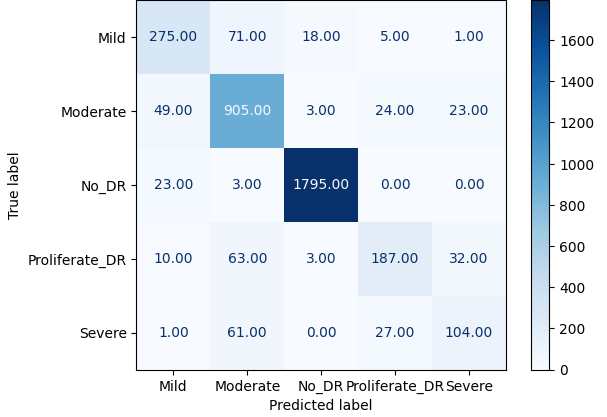
\includegraphics[width=0.66\linewidth]{hybrid_confusion_5class}
\caption[Confusion matrix of the hybrid model on five-class grading]{Confusion matrix of the
hybrid CNN--GNN model on five-class grading (APTOS~2019). Correct predictions lie on the
diagonal; most errors are between Severe and Proliferative DR. Adapted
from~\cite{mezghich2026lnaitopo}.}
\label{fig:hybridcm}
\end{figure}

\begin{figure}[!tb]
\centering
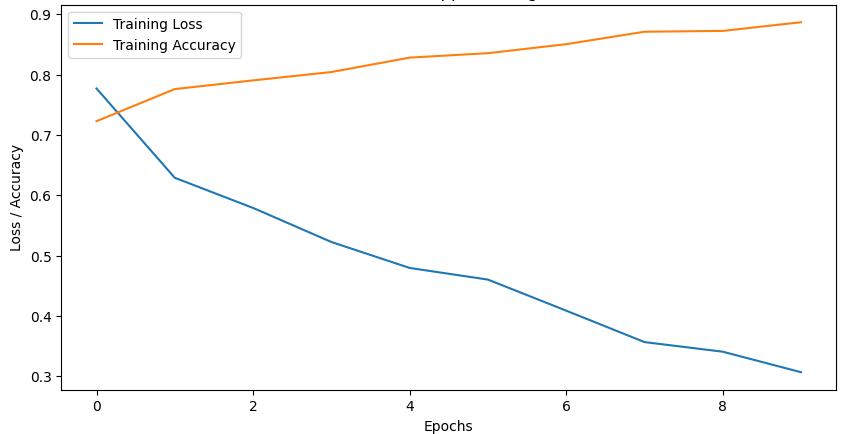
\includegraphics[width=0.78\linewidth]{hybrid_training_curves}
\caption[Training curves of the hybrid model]{Training loss and training accuracy of the
hybrid CNN--GNN model on five-class grading, per epoch. Adapted
from~\cite{mezghich2026lnaitopo}.}
\label{fig:hybridcurves}
\end{figure}

\paragraph{Topological descriptors of the vessel skeleton.}
The later systems of this thesis describe the vascular network with a fixed vector of
persistence statistics. For each fundus image, the vessel skeleton is extracted with CLAHE
pre-processing~\cite{zuiderveld1994clahe} followed by Zhang--Suen
thinning~\cite{zhang1984thinning}. The branch points of the skeleton form a point cloud
$P_i=\{p_1,\ldots,p_n\}\subset\mathbb{R}^2$. The Vietoris--Rips filtration is computed
with GUDHI~\cite{maria2014gudhi}, which gives a seven-dimensional feature vector
\begin{equation}
x_i^{\mathrm{TDA}} = \bigl(\Pi_{H_0},\, n_{H_0},\, \Pi_{H_1},\, n_{H_1},\, \beta_1,\,
D_f,\, \Delta\bigr)^\top \in \mathbb{R}^7 ,
\label{eq:tda}
\end{equation}
where $\Pi_{H_k}$ is the total $k$-th persistence, $n_{H_k}$ the number of components
or loops, $\beta_1$ the first Betti number, $D_f$ the fractal dimension, and $\Delta$ the
maximum $H_1$ persistence (a neovascularisation signal).

The synergy observed in \cref{tab:hybrid} motivates the next step. In the hybrid model,
the graph links positions within one image and the topological descriptors are simply
concatenated; TOPORET (\cref{sec:dualsim}) instead builds a graph between patients and uses
the distance between persistence diagrams inside the similarity that defines its edges,
fusing both signals at graph-construction time.

\subsection{SAMF-GB: Structural Features Outperform GPU EfficientNet-B3}
\label{sec:samfgb}

SAMF-GB~\cite{belhadj2026samfgb} shows that seven families of hand-crafted structural
features, combined with LightGBM gradient boosting~\cite{ke2017lightgbm}, outperform a
GPU EfficientNet-B3 at about $1/13$ of the computational cost. The 256-dimensional
feature vector is composed as follows:
\begin{itemize}
\item \textbf{vascular morphology} (48-D): vessel calibre reduction and tortuosity;
\item \textbf{fractal dimension} (12-D): loss of vascular self-similarity;
\item \textbf{persistent homology} (7-D): topology of the vessel network (\cref{eq:tda});
\item \textbf{DWT texture} (64-D, four levels): microaneurysm and exudate texture;
\item \textbf{Gabor responses} (32-D): vessel edges and IRMA characteristics;
\item \textbf{radial FFT} (24-D): degradation of the spoke-wheel vessel pattern;
\item \textbf{LBP $+$ log-Euclidean} (69-D): haemorrhage and exudate cluster patterns.
\end{itemize}

\Cref{tab:shap} gives the dimension and mean absolute SHAP value~\cite{lundberg2017shap}
of each family. The three most discriminative families are all global structural
features (vascular morphology, fractal dimension, persistent homology), not local
appearance features. This is independent evidence for H2, obtained with a method entirely
different from the ANOVA of \cref{sec:h2}.

\begin{table}[H]
\centering
\caption[SAMF-GB feature families and mean absolute SHAP values]{SAMF-GB feature families, dimension and mean absolute SHAP
value~\cite{belhadj2026samfgb}.}
\label{tab:shap}
\small
\begin{tabular}{@{}lccP{6.2cm}@{}}
\toprule
Family & Dim. & Mean $|\mathrm{SHAP}|$ & Primary DR correlate \\
\midrule
Vascular morphology & 48 & 0.142 & Vessel calibre reduction, tortuosity \\
Fractal dimension & 12 & 0.138 & Loss of vascular self-similarity \\
Persistent homology & 7 & 0.131 & Topology of the vascular network \\
DWT (4 levels) & 64 & 0.094 & Microaneurysm and exudate texture \\
Gabor responses & 32 & 0.087 & Vessel edges and IRMA \\
Radial FFT & 24 & 0.082 & Spoke-wheel vessel pattern degradation \\
LBP $+$ log-Euclidean & 69 & 0.068 & Haemorrhage and exudate clusters \\
\midrule
Full SAMF-GB & 256 & -- & QWK $=0.882$; $2.1$~ms CPU inference \\
\bottomrule
\end{tabular}
\end{table}

The SHAP ranking of \cref{tab:shap} is also a check on the clinical plausibility of the
model: the three families that matter most describe the geometry and topology of the
vessels, which are the structures that ophthalmologists examine when they look for venous
beading, capillary closure and new vessels.

\Cref{tab:samf} compares SAMF-GB with
EfficientNet-B3: SAMF-GB gains $+0.042$ QWK, its classifier runs on a 16-core CPU instead
of a GPU at about 13 times lower cost, and its predictions can be explained with SHAP.

\begin{table}[H]
\centering
\caption[SAMF-GB versus EfficientNet-B3 on Kaggle EyePACS]{SAMF-GB versus EfficientNet-B3 on Kaggle EyePACS ($N=88{,}702$).}
\label{tab:samf}
\small
\begin{tabular}{@{}lcccl@{}}
\toprule
System & QWK & Inference & Hardware & Art.~13 support \\
\midrule
EfficientNet-B3 & 0.840 & 85~ms & NVIDIA A100 & No (opaque) \\
SAMF-GB & 0.882 & 2.1~ms & 16-core CPU & Yes (SHAP per prediction) \\
\midrule
Difference & $+0.042$ & $\times 40$ (classifier only) & $\times 13$ cheaper & -- \\
\bottomrule
\end{tabular}
\tabnote{The $2.1$~ms of SAMF-GB is the inference time of the gradient-boosting model on
pre-computed features. Feature extraction is not included: the persistent-homology stage
alone takes about $18$~ms per image on the same CPU (\cref{tab:latency}). The speed ratio
therefore compares classifiers, not complete pipelines.}
\end{table}

\subsection{LightGBM-HC}
\label{sec:lgbmhc}

Publication~\cite{belhadj2026icpram} validates a reduced 128-dimensional hand-crafted
feature set with LightGBM, reaching QWK $=0.858$ at $1.6$~ms CPU inference on the same
benchmark. The hyperparameters, each selected by five-fold cross-validated grid search,
are listed in \cref{tab:lgbm-hp}. The QWK is lower than that of SAMF-GB ($0.858$ versus $0.882$, a difference of $0.024$).
LightGBM-HC omits the 7-D persistent-homology features, but also the radial FFT and
LBP families and most of the Gabor responses; the difference therefore cannot be
attributed to topology alone. It is consistent with, but does not isolate, a contribution
of the topological component; the isolated contribution of the TDA features is measured
in the TOPORET ablation ($+0.016$ QWK, \cref{tab:ablation3}).

\begin{table}[H]
\centering
\caption[LightGBM-HC hyperparameters]{LightGBM-HC hyperparameters, selected by five-fold cross-validated grid search on
Kaggle EyePACS (search range in parentheses).}
\label{tab:lgbm-hp}
\small
\begin{tabular}{@{}ll@{}}
\toprule
Hyperparameter & Selected value (search range) \\
\midrule
Number of boosting rounds & 480 (100--1000) \\
Maximum tree depth & 7 (3--12) \\
Learning rate & 0.04 (0.01--0.2, log scale) \\
Number of leaves & 63 (15--127) \\
Minimum child samples & 20 (5--50) \\
Feature subsampling fraction & 0.75 (0.5--1.0) \\
L2 regularisation & 1.2 (0--5) \\
\bottomrule
\end{tabular}
\end{table}

\paragraph{Feature-family ablation.}
To isolate the contribution of each of the four families retained in the 128-D set
(vascular morphology, fractal dimension, DWT texture, Gabor responses), a
leave-one-family-out ablation was run (\cref{tab:lgbm-abl}). Vascular morphology is by
far the most load-bearing family ($-0.077$ QWK when removed), more than the two
texture-oriented families together. This agrees with the SHAP ranking of SAMF-GB and
reaches the same conclusion by a different method: global vascular structure carries more
signal than local texture for this task.

\begin{table}[!tb]
\centering
\caption[Leave-one-family-out ablation for LightGBM-HC]{Leave-one-family-out ablation for LightGBM-HC. Each row removes one family from
the 128-D set.}
\label{tab:lgbm-abl}
\small
\begin{tabular}{@{}lcc@{}}
\toprule
Configuration & QWK & $\Delta$ vs.\ full set \\
\midrule
Full 128-D feature set & 0.858 & -- \\
$-$ Vascular morphology (48-D) & 0.781 & $-0.077$ \\
$-$ Fractal dimension (12-D) & 0.829 & $-0.029$ \\
$-$ DWT texture (64-D) & 0.842 & $-0.016$ \\
$-$ Gabor responses (4-D, reduced) & 0.851 & $-0.007$ \\
\bottomrule
\end{tabular}
\end{table}

With only four families and $128$ dimensions, LightGBM-HC keeps most of the accuracy of
SAMF-GB at a lower cost, which makes it a practical option for screening sites equipped only
with standard computers. Both gradient-boosting models also provide feature-level explanations directly, without any post-hoc method.

\subsection{Convergent Evidence from Four Independent Methodologies}
\label{sec:converge}

Four methodologically independent approaches --- the three studies of Part~B and the
formal ANOVA of \cref{ch:toporet} --- reach the same qualitative conclusion:
global structural priors improve DR grading.
\begin{enumerate}
\item \textbf{Deep learning}~\cite{belhadj2026hybrid,mezghich2026lnaitopo}: topological descriptors add $+1.7$~pp
beyond the CNN baseline (\cref{tab:hybrid}).
\item \textbf{Gradient boosting}~\cite{belhadj2026samfgb}: SAMF-GB outperforms GPU
EfficientNet-B3 by $+0.042$ QWK at about 13 times lower cost; topology ranks third of
seven families by SHAP (\cref{tab:shap}).
\item \textbf{Reduced gradient boosting}~\cite{belhadj2026icpram}: the reduced feature set
without topology (and without three other families) loses $0.024$ QWK, and the
leave-one-family-out ablation ranks global vascular morphology first
(\cref{tab:lgbm-abl}).
\item \textbf{Formal ANOVA} (\cref{sec:h2}): $F(4,4995)=1308.9$, $\eta^2=0.51$.
\end{enumerate}

\paragraph{Why four methodologies, not one.}
One could ask whether a single, larger experiment would have established the same point
with less apparent duplication. Four methodologies were used because each has its own
characteristic failure mode, and agreement across methods with different failure modes is
harder to explain away than one large effect. A deep-learning ablation
(\cref{tab:hybrid}) can be confounded by optimisation idiosyncrasies; a SHAP attribution
(\cref{tab:shap}) by correlated features inflating or deflating attributions; a
leave-one-family-out ablation (\cref{tab:lgbm-abl}) by interactions between the removed
and retained families. No single confound threatens all four at once, so their agreement
is correspondingly hard to attribute to a methodological artefact. The same logic
motivates the distributed-systems detour of Part~A: breadth of independent evidence,
rather than depth within one experimental paradigm, is the organising principle of the
evidential strategy of this thesis. The same principle guides the evaluation of TOPORET and DOTS in the next chapters.

\section{Synthesis of the First Contributions}
\label{sec:ch3-synthesis}

\Cref{tab:ch3summary} summarises the five studies of this chapter.

Three design decisions for the rest of the thesis follow directly from these studies. The
graph template, its hyperparameters and its inductive mode can be reused unchanged on
retinal data, since they proved stable across six domains. Topological descriptors of the
vessel skeleton deserve a place in the model, since three different methods found them
informative. Finally, the way the two signals are combined matters: since they are already synergistic
when simply concatenated, the next system goes further and fuses topology into the
similarity that builds a graph between patients. The remainder of this section summarises the evidence on which these decisions rest.

\begin{table}[H]
\centering
\caption{Summary of the first contributions.}
\label{tab:ch3summary}
\small
\begin{tabular}{@{}P{3.6cm} P{3.4cm} P{5.2cm} c@{}}
\toprule
Study & Data & Main result & Publication \\
\midrule
GNN-MSOrchest & 48-service microservice simulation & Cascade containment $81\%$ vs.\ $34\%$ & P1 \\
Structural invariants & Six graph benchmarks & Mean recall $+4.2$~pp, CV $14\%$ & P2 \\
Hybrid CNN--GNN & APTOS 2019 (binary) & $95.1\%$ accuracy ($+7.0$~pp), AUC $0.970$; synergistic gains & P3, B2 \\
SAMF-GB & Kaggle EyePACS & QWK $0.882$ vs.\ $0.840$; CPU classifier ($2.1$~ms) & J2 \\
LightGBM-HC & Kaggle EyePACS & QWK $0.858$ with a reduced 128-D set & P4 \\
\bottomrule
\end{tabular}
\end{table}

\section*{Conclusion}
\phantomsection\addcontentsline{toc}{section}{Conclusion}

This chapter established three empirical findings. (F1)~The GraphSAGE template with
structural descriptors gives stable gains on six heterogeneous benchmarks
(mean recall gain $+4.2$~pp, coefficient of variation $14\%$). (F2)~On DR data, relational and
topological contributions are complementary: the full hybrid model gains $+7.0$~pp over the
CNN baseline, more than the sum of the individual gains ($6.3$~pp). (F3)~Global
structural and topological features carry discriminative information, as shown
independently by a deep hybrid model, by gradient boosting with SHAP attribution and by a
leave-one-family-out ablation. As a practical by-product, SAMF-GB reaches a higher QWK than a GPU EfficientNet-B3 with a
gradient-boosting classifier that runs on a standard CPU ($2.1$~ms per image once the
features are extracted).

These results do not prove that a population graph will work on retinal images, but they
show that it is worth testing, with topology fused into the similarity that builds the
graph. The next chapter implements this idea in TOPORET.

\chapter{Topology-Aware Population Graph for Diabetic Retinopathy Grading}
\label{ch:toporet}
\lofgroup{Chapter 4 -- Topology-Aware Population Graph for Diabetic Retinopathy Grading}
\lotgroup{Chapter 4 -- Topology-Aware Population Graph for Diabetic Retinopathy Grading}
\section*{Introduction}
\phantomsection\addcontentsline{toc}{section}{Introduction}

The previous chapter showed that global structural features carry useful information for
DR grading, and that graph and topological signals should be fused rather than simply
concatenated. This chapter turns these observations into a complete grading framework,
TOPORET~\cite{belhadj2025plos}. TOPORET connects patients in an inductive population graph
whose edges combine two similarities: how alike the fundus images look to a CNN, and how
alike their vessel networks are topologically. This thesis introduces it as a DR grading
system that addresses the relational limitation (L1) and the structural limitation (L2)
at the same time; we are not aware of an earlier system combining these two elements in a
single inductive population graph.

We first review related work on population graphs and topological features in medical
imaging. We then state the two hypotheses tested in this chapter, present the six-stage
pipeline and the dual-similarity graph, and report the experiments: statistical tests of
the hypotheses, analysis of the graph, ablation, cross-dataset evaluation and comparison
with the literature. We close with a discussion of what the results do and do not imply.

\section{Related Work}
\label{sec:ch3-related}

\paragraph{Population graphs in medical imaging.}
Representing a cohort as a graph whose nodes are patients was popularised for disease
prediction from brain imaging, where graph convolutional networks combine imaging features
with phenotypic similarity between subjects~\cite{parisot2018disease}. The idea is that
similar patients tend to share a diagnosis, so the graph can propagate information from
labelled to unlabelled subjects. These approaches are usually transductive: the whole
cohort, including the test patients, must be present when the model is trained, which is
not compatible with a screening service where new patients arrive every day. In the DR
grading work reviewed here, graph-based approaches have used visual similarity only; we re-implement such a
visual-only graph (GraphDR) as the control of this chapter.

\paragraph{Topological features in medical imaging.}
Persistent homology has been used to describe the shape of anatomical structures and to
feed learning models with stable, interpretable descriptors~\cite{hofer2017topological,
carriere2020perslay}. For the retina, the complexity of the vascular tree, often summarised
by its fractal dimension~\cite{masters2004fractal}, is known to change with disease. To our
knowledge, persistence descriptors of the vessel skeleton had not been used as edge
information in a population graph before this work.

\section{Problem Formulation and Hypotheses}
\label{sec:ch3-problem}\label{sec:hyp}

Let $\{(I_j,y_j)\}$ be a set of fundus images with ICDR grades $y_j\in\{0,\ldots,4\}$. The
task is to predict the grade $\hat y_i$ of a new image $I_i$ that was not seen during
training, using both its own content and the content of similar patients. The chapter tests
two pre-specified hypotheses; their decision thresholds were fixed before any data were
analysed.

\paragraph{H1 -- The Relational Hypothesis.}
An inductive population graph connecting patients through a dual-similarity metric
(visual embedding similarity $+$ Wasserstein topological distance) provides a
statistically significant QWK improvement over independent per-image classification.
\emph{Pre-specified test:} paired $t$-test across five cross-validation folds, TOPORET
versus EfficientNet-B3; null hypothesis $\mu_{\Delta\mathrm{QWK}} \leq 0$. The nominal
one-tailed critical value is $t_{0.05,4}=2.132$; the more conservative $t_4 > 2.78$
($t_{0.025,4}$) was adopted as the decision threshold.

\paragraph{H2 -- The Structural Hypothesis.}
$H_0$ and $H_1$ persistent-homology features of the retinal vascular skeleton are
associated with ICDR severity grade.
\emph{Pre-specified test:} one-way ANOVA across the five grades ($n=5{,}000$), Tukey HSD
post-hoc, Bonferroni-corrected significance level $\alpha=0.005$; critical value
$F_{0.005;\,4,4995}=3.72$.

\section{Proposed Approach}
\label{sec:ch3-approach}

\subsection{Overview}
\label{sec:ch3-overview}

TOPORET~\cite{belhadj2025plos} addresses L1 with a population graph and L2 with
persistent homology, in a single pipeline.
\Cref{fig:toporet} shows its six stages, the typed interface between consecutive stages,
and its headline results.

Three design principles guide TOPORET. First, the graph is \emph{inductive}: a new patient
is connected to the existing cohort at inference time, without retraining, which is what a
screening service requires. Second, topology is used twice: as a feature of each patient
and inside the similarity that decides which patients are neighbours, which extends the
synergy observed in \cref{ch:found} from a single image to the whole population. Third, each
stage has a typed input and output, so that it can be tested, replaced or audited on its
own; this modularity is reused unchanged by DOTS in \cref{ch:dots}.

% Figure 3.1 --- TOPORET six-stage pipeline
\begin{figure}[!htbp]
\centering
\resizebox{\linewidth}{!}{%
\begin{tikzpicture}[
  font=\footnotesize,
  box/.style={draw, rounded corners=2pt, align=center, inner sep=2.5pt,
              minimum height=1.6cm, text width=1.58cm},
  arr/.style={-{Latex[length=2.2mm]}, thick}
]
\node[box, fill=black!6, draw=black!55] (s1) {\textbf{S1}\\CLAHE $+$\\skeleton};
\node[box, fill=black!6, draw=black!55, right=2.2mm of s1] (s2) {\textbf{S2}\\EffNet-B3\\(frozen)};
\node[box, fill=axisSf, draw=axisS, right=2.2mm of s2] (s3) {\textbf{S3}\\Rips\\TDA 6-D};
\node[box, fill=fusionf, draw=fusion, right=2.2mm of s3] (s4) {\textbf{S4}\\Fusion\\1542-D};
\node[box, fill=axisRf, draw=axisR, right=2.2mm of s4] (s5) {\textbf{S5}\\Dual-sim.\\graph ($\tau$)};
\node[box, fill=axisRf, draw=axisR, right=2.2mm of s5] (s6) {\textbf{S6}\\{\scriptsize GraphSAGE}\\$+$ softmax};
\foreach \a/\b in {s1/s2,s2/s3,s3/s4,s4/s5,s5/s6} \draw[arr] (\a) -- (\b);
\node[left=2.5mm of s1, font=\footnotesize, align=center] (in) {Fundus\\image $I_i$};
\node[right=2.5mm of s6, font=\footnotesize, align=center] (out) {Grade\\$\hat y_i$};
\draw[arr] (in) -- (s1); \draw[arr] (s6) -- (out);
\node[below=6mm of s3.south east, anchor=north, font=\footnotesize, align=center] {%
  Kaggle DR: QWK $=0.88$, accuracy $95.5\%$ (five-fold cross-validation)\\H1: $t_4=3.82$ \quad H2: $F=84.3$, $p<0.001$};
\end{tikzpicture}}
\caption[TOPORET six-stage pipeline]{TOPORET six-stage pipeline. Blue stages form the relational axis (L1), the green
stage the structural axis (L2). There is no ordinal-safety axis: every image is graded
and the order of the grades is not modelled. Stage contracts are given in
\cref{tab:stages}; results from~\cite{belhadj2025plos}.}
\label{fig:toporet}
\end{figure}


\subsection{Six-Stage Pipeline}
\label{sec:stages}

\Cref{tab:stages} gives the typed input/output contract of each stage. The contracts are
what makes each stage unit-testable in isolation (\cref{sec:iec62304}).

\begin{table}[H]
\centering
\caption[TOPORET six-stage modular pipeline]{TOPORET six-stage modular pipeline. Each stage has a typed interface contract
that supports IEC~62304 unit verification.}
\label{tab:stages}
\small
\begin{tabular}{@{}c l P{4.6cm} P{4.4cm}@{}}
\toprule
Stage & Name & Input $\to$ Output & Key operation \\
\midrule
S1 & Pre-processing & Fundus image $\to$ enhanced image $+$ skeleton & CLAHE $+$ Zhang--Suen thinning \\
S2 & CNN extraction & Enhanced image $\to$ $x_i^{\mathrm{CNN}}\in\mathbb{R}^{1536}$ & EfficientNet-B3 (frozen) \\
S3 & TDA persistence & Skeleton points $\to$ $x_i^{\mathrm{TDA}}\in\mathbb{R}^{7}$ & GUDHI Vietoris--Rips, \cref{eq:tda} \\
S4 & Feature fusion & $x_i^{\mathrm{CNN}}, x_i^{\mathrm{TDA}} \to z_i\in\mathbb{R}^{1543}$ & Concatenation \\
S5 & Graph construction & $\{z_i\}\to G=(V,E,S_{ij})$ & FAISS $k$-NN, dual similarity \\
S6 & GNN inference & $G, z_i \to \hat y_i$ & GraphSAGE $+$ CORN ordinal head \\
\bottomrule
\end{tabular}
\end{table}

\Cref{fig:skeleton} follows stages S1--S3 on one fundus image. Panel~(a) is the segmented
vessel network; panel~(b) its one-pixel skeleton $P_i$, obtained by Zhang--Suen
thinning~\cite{zhang1984thinning}; panel~(c) the persistence diagram $D_i$ of the
Vietoris--Rips filtration built on the skeleton points, in which filled dots are $H_0$
components and open dots are $H_1$ loops. The 7-D vector of \cref{eq:tda} is computed
from this diagram.

\begin{figure}[!tb]
\centering
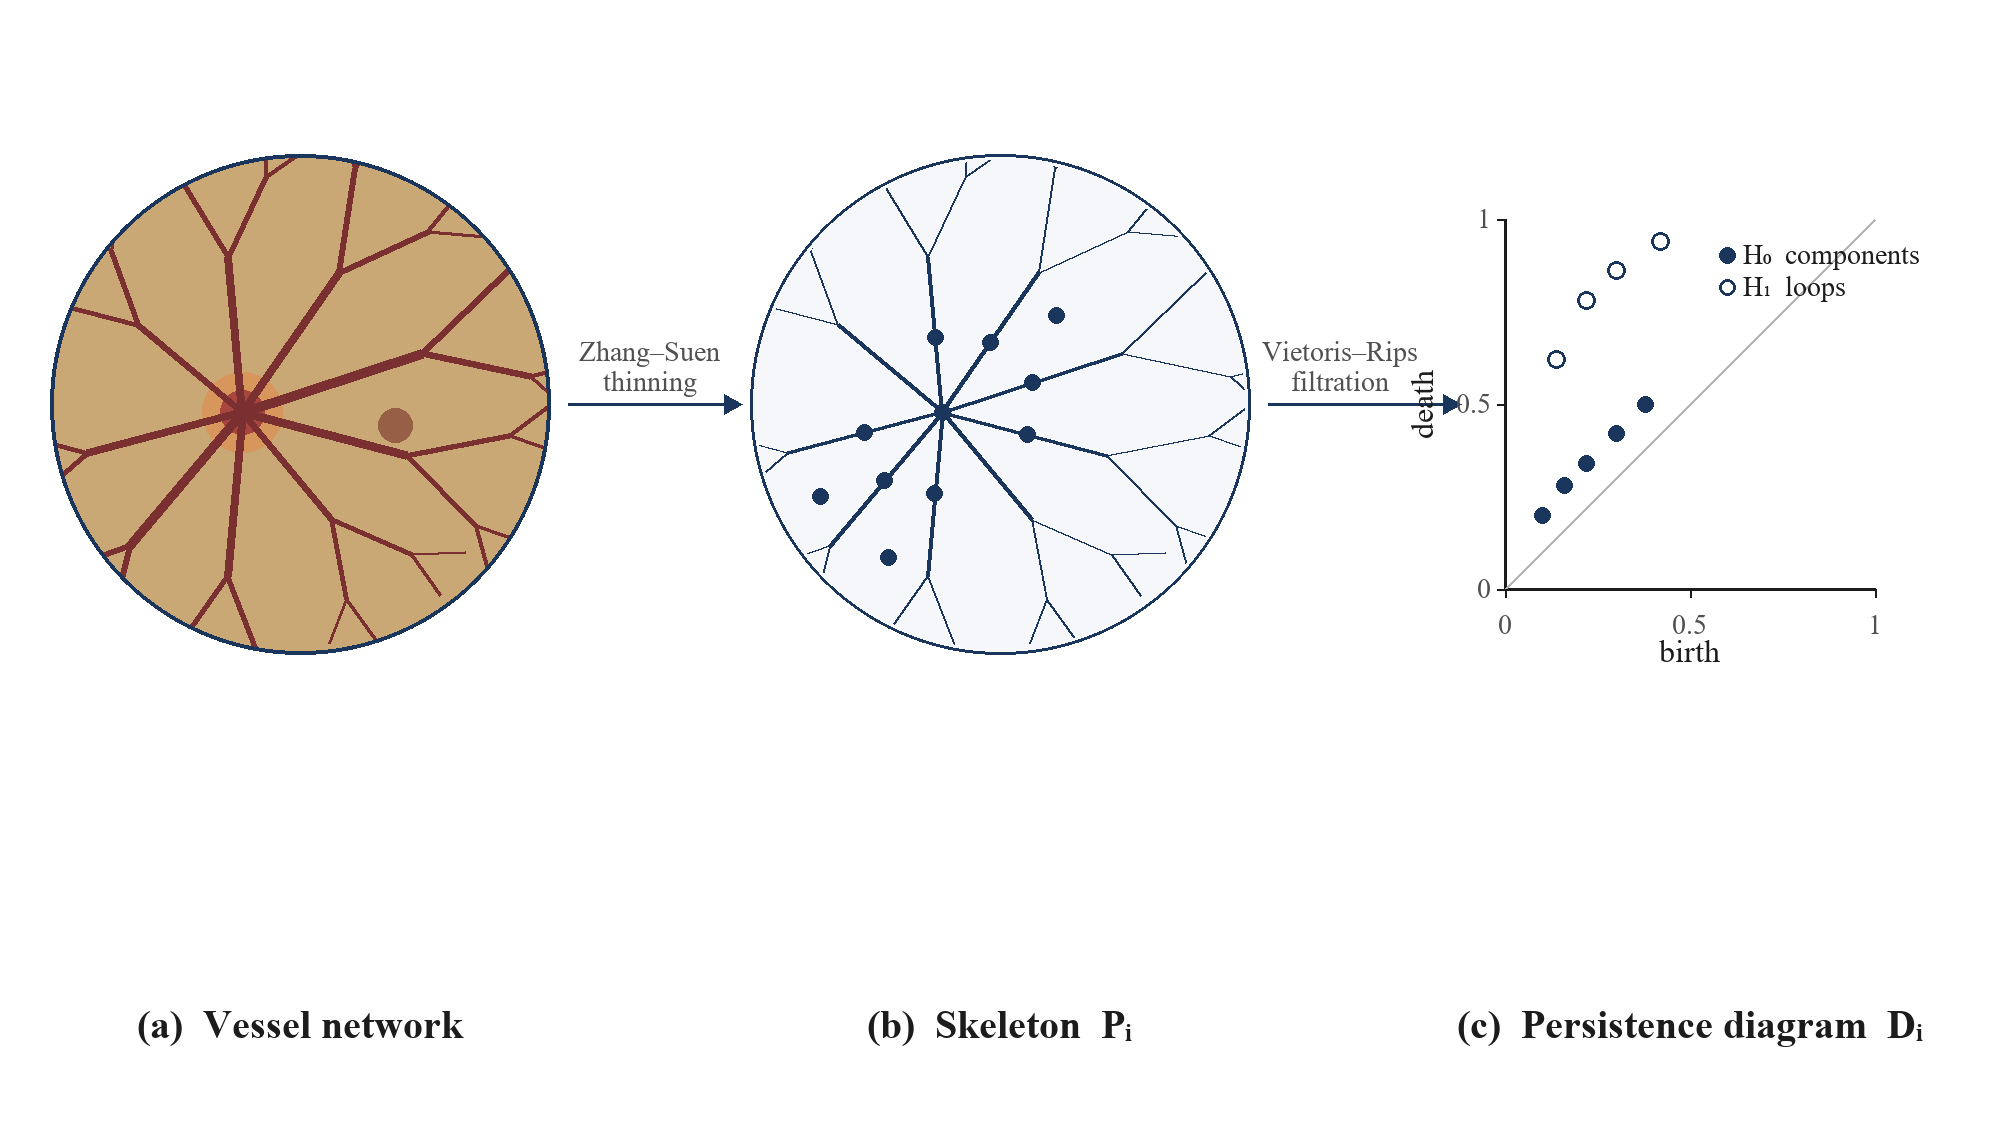
\includegraphics[width=0.86\textwidth]{vessel_skeleton_persistence}
\caption[Vessel skeleton extraction and topological features (stages S1--S3)]{Vessel skeleton extraction and topological features (stages S1--S3):
(a)~vessel network, (b)~Zhang--Suen skeleton $P_i$, (c)~Vietoris--Rips persistence
diagram $D_i$ (filled: $H_0$ components; open: $H_1$ loops).}
\label{fig:skeleton}
\end{figure}

\Cref{fig:clahe} shows the first operation of stage S1 on a Grade~2 image: the photograph
as acquired and the same image after CLAHE~\cite{zuiderveld1994clahe} with clip limit
$2.0$ and an $8\times 8$ tile grid. Local contrast enhancement sharpens the boundaries of
microaneurysms and haemorrhages and separates the vessels from the background. This makes
the vessel segmentation and skeleton extracted later in stage S1 more reliable, without
saturating healthy tissue or shifting the global colour balance.

\begin{figure}[H]
\centering
\begin{minipage}{0.86\textwidth}
\begin{subfigure}[t]{0.4\textwidth}\centering
  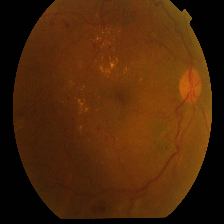
\includegraphics[width=\linewidth,height=\linewidth,keepaspectratio]{clahe_original}
  \caption{Original, as acquired}
\end{subfigure}\hfill
\begin{subfigure}[t]{0.4\textwidth}\centering
  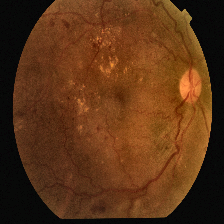
\includegraphics[width=\linewidth,height=\linewidth,keepaspectratio]{clahe_enhanced}
  \caption{After CLAHE (clip 2.0, $8\times8$)}
\end{subfigure}
\end{minipage}
\caption[Effect of CLAHE pre-processing on a Grade~2 fundus image]{Effect of CLAHE pre-processing (stage S1) on a Grade~2 fundus image: (a)~original, (b)~after CLAHE with clip limit $2.0$ and an $8\times8$ tile grid.}
\label{fig:clahe}
\end{figure}

\subsection{Dual-Similarity Population Graph}
\label{sec:dualsim}

The dual-similarity edge weight combines the cosine similarity of visual embeddings with
a Wasserstein topological term:
\begin{equation}
S_{ij} = \alpha\cdot\cos\bigl(x_i^{\mathrm{CNN}},\, x_j^{\mathrm{CNN}}\bigr)
       + (1-\alpha)\cdot\exp\bigl(-W_2(D_i, D_j)\bigr),
\label{eq:dualsim}
\end{equation}
with $\alpha=0.65$ and $k=15$ neighbours, both selected by five-fold cross-validation.
\Cref{tab:hparam} reports the QWK stability of each hyperparameter over its range: every
hyperparameter moves QWK by at most $0.5$~pp inside the stable interval, so the results
are not a knife-edge consequence of one setting.

\begin{table}[H]
\centering
\caption[Hyperparameter sensitivity of TOPORET]{Hyperparameter sensitivity of TOPORET: QWK stability over the tested range.}
\label{tab:hparam}
\small
\begin{tabular}{@{}lllc@{}}
\toprule
Hyperparameter & Range tested & QWK stability & Selected \\
\midrule
$\alpha$ (visual/topological balance) & $[0.3,\,0.9]$ & $\pm0.5$~pp over $[0.5,\,0.8]$ & 0.65 \\
$k$ (neighbours) & $\{5,8,10,15,20\}$ & $\pm0.3$~pp over $[8,\,15]$ & 15 \\
$d_h$ (hidden dimension) & $\{128,256,512\}$ & $\pm0.2$~pp & 256 \\
$p$ (dropout) & $[0.1,\,0.5]$ & $\pm0.4$~pp over $[0.2,\,0.5]$ & 0.30 \\
\bottomrule
\end{tabular}
\end{table}

\Cref{alg:toporet} summarises how TOPORET builds the population graph and grades a new
patient. Training images are processed once; a new image only requires its own features,
a $k$-nearest-neighbour query and one GraphSAGE forward pass.

\begin{algorithm}[!htb]
\caption{TOPORET: population-graph construction and inductive grading.}
\label{alg:toporet}
\DontPrintSemicolon
\KwIn{training images $\{I_j\}$ with grades $\{y_j\}$; new image $I_i$; parameters $\alpha=0.65$, $k=15$}
\KwOut{predicted grade $\hat y_i$}
\BlankLine
\ForEach{training image $I_j$}{
  $\tilde I_j \leftarrow \mathrm{CLAHE}(I_j)$; $P_j \leftarrow \mathrm{Skeleton}(\tilde I_j)$\tcp*{stage S1}
  $x_j^{\mathrm{CNN}} \leftarrow \mathrm{EfficientNetB3}(\tilde I_j)$\tcp*{stage S2}
  $D_j \leftarrow \mathrm{RipsPersistence}(P_j)$; $x_j^{\mathrm{TDA}} \leftarrow \phi(D_j)$\tcp*{stage S3, \cref{eq:tda}}
  $z_j \leftarrow [\,x_j^{\mathrm{CNN}} \Vert x_j^{\mathrm{TDA}}\,]$\tcp*{stage S4}
}
Build the graph $G$: connect each node to its $k$ most similar nodes under $S_{ij}$ (\cref{eq:dualsim})\tcp*{stage S5}
Train GraphSAGE with a CORN ordinal head on $G$ (five-fold cross-validation)\tcp*{stage S6}
\BlankLine
Compute $z_i$ for the new image $I_i$ with stages S1--S4\;
$\mathcal{N}(i) \leftarrow$ the $k$ training nodes with highest $S_{ij}$ (FAISS query)\;
$h_i \leftarrow \mathrm{GraphSAGE}(z_i,\{z_j\}_{j\in\mathcal{N}(i)})$\tcp*{\cref{eq:sage-agg,eq:sage-upd}}
\Return{$\hat y_i \leftarrow \mathrm{CORN}(h_i)$}
\end{algorithm}

\subsection{Design Choices}
\label{sec:ch3-design}

Several alternatives were possible at each stage of TOPORET. This subsection explains the
choices made and the reasons behind them.

\paragraph{Inductive rather than transductive learning.}
Population-graph methods in medical imaging are often transductive: the test patients are
part of the graph during training~\cite{parisot2018disease}. This is convenient for a
research study but incompatible with a screening service, where new patients arrive every
day and retraining the model for each of them is not possible. GraphSAGE was chosen
because it learns an aggregation \emph{function} rather than node-specific embeddings, so
that a new patient can be graded by connecting it to the existing graph and applying the
learned function (\cref{sec:sage}).

\paragraph{Topology computed on vessel branch points.}
Persistent homology can be computed directly on the image intensities, using cubical
complexes, or on a point cloud extracted from the image. The first option captures every
bright or dark structure, including lesions, illumination gradients and noise. Computing
the Vietoris--Rips filtration on the branch points of the vessel skeleton restricts the
analysis to the object of interest, the vascular network, and produces features that can
be interpreted in vascular terms (\cref{sec:tda-bio}). The price is a dependence on the
quality of the segmentation and thinning, which is mitigated by CLAHE pre-processing and
by the stability of persistence diagrams (\cref{eq:stability}).

\paragraph{A small vector of summary statistics.}
Richer representations of persistence diagrams exist, such as persistence landscapes or
images, and learned layers can process diagrams directly (\cref{sec:ph}). A seven-dimensional
vector of summary statistics was preferred for two reasons: each component has a direct
clinical interpretation, which matters for transparency, and the small dimension keeps the
topological signal from being drowned by the $1536$ dimensions of the CNN embedding when
the two are concatenated.

\paragraph{Similarity fused at graph-construction time.}
The hybrid model of \cref{ch:found} concatenated graph and topological signals and found
their gains synergistic. TOPORET goes further and uses topology inside the edge weights
(\cref{eq:dualsim}), so that two patients are connected only if their images look alike
\emph{and} their vessel networks have a similar shape. The Wasserstein distance was chosen
to compare diagrams because it takes all points of the diagrams into account, not only the
largest difference as the bottleneck distance does. The balance $\alpha$ between the two
terms was selected by cross-validation rather than fixed a priori.

\paragraph{Approximate nearest neighbours.}
Connecting each patient to its $k$ most similar patients requires a nearest-neighbour
search among tens of thousands of embeddings. An exact search would grow linearly with the
cohort; the FAISS library~\cite{johnson2021faiss} provides approximate search with
negligible loss of accuracy and a query time of about a millisecond, which keeps the
per-patient cost of TOPORET independent of the cohort size. Together, these choices keep TOPORET simple enough to be verified stage by stage, which prepares the engineering work of \cref{ch:reg}.

\section{Experimentation}
\label{sec:ch3-exp}

\subsection{Datasets and Protocol}

All experiments use Kaggle EyePACS~\cite{kaggle2015eyepacs} ($N=88{,}702$) for training
and in-distribution evaluation, with five folds stratified by ICDR grade and a fixed random
seed. Out-of-distribution generalisation is measured on Messidor-2~\cite{decenciere2014messidor}
and IDRiD~\cite{porwal2018idrid}, which come from other countries and cameras. The ANOVA of
H2 uses a stratified sample of $5{,}000$ images ($1{,}000$ per grade). Three systems are
compared throughout: EfficientNet-B3 alone, the visual-only graph (GraphDR) and TOPORET.
The hyperparameters were selected on the training folds only (\cref{tab:hparam}).

\subsection{Results: Topological Features and Severity (H2)}
\label{sec:h2}

\paragraph{Pre-specified test.}
One-way ANOVA on each of the six TDA features of \cref{tab:anova} across the five ICDR
grades ($n=5{,}000$, 1{,}000 images per grade, stratified from Kaggle EyePACS), with
Tukey HSD post-hoc comparisons~\cite{tukey1949} and a Bonferroni-corrected significance
level. The Bonferroni level for six features is $0.05/6\approx0.0083$; the more
conservative $\alpha=0.005$ was pre-specified, with critical value
$F_{0.005;\,4,4995}=3.72$.

\begin{table}[H]
\centering
\caption[ANOVA of the topological features across ICDR grades]{One-way ANOVA of the topological features across the five ICDR grades
($n=5{,}000$, Kaggle EyePACS). Values are mean $\pm$ SD.}
\label{tab:anova}
\small
\setlength{\tabcolsep}{4pt}
\begin{tabular}{@{}lccccccc@{}}
\toprule
Feature & G0 & G1 & G2 & G3 & G4 & $F(4,4995)$ & $\eta^2$ \\
\midrule
$\Pi_{H_0}$ & $24.3\pm3.1$ & $23.1\pm3.4$ & $21.6\pm3.7$ & $19.8\pm4.0$ & $18.7\pm4.2$ & $385.8^{***}$ & 0.24 \\
$\Pi_{H_1}$ & $8.2\pm1.4$ & $9.4\pm1.8$ & $11.2\pm2.3$ & $13.5\pm3.1$ & $15.6\pm3.8$ & $1308.9^{***}$ & 0.51 \\
$n_{H_0}$ & $142\pm18$ & $136\pm19$ & $127\pm21$ & $118\pm23$ & $109\pm25$ & $388.8^{***}$ & 0.24 \\
$\beta_1$ & $1.8\pm0.6$ & $2.3\pm0.8$ & $3.1\pm1.0$ & $4.0\pm1.3$ & $4.8\pm1.5$ & $1258.4^{***}$ & 0.50 \\
$D_f$ & $1.71\pm0.04$ & $1.68\pm0.05$ & $1.64\pm0.05$ & $1.60\pm0.06$ & $1.57\pm0.06$ & $1177.5^{***}$ & 0.49 \\
$\Delta$ & $0.8\pm0.3$ & $1.1\pm0.4$ & $1.5\pm0.6$ & $2.2\pm0.9$ & $3.8\pm1.3$ & $2294.2^{***}$ & 0.65 \\
\bottomrule
\end{tabular}
\tabnote{$^{***}p<0.001$. Critical value $F_{0.005;\,4,4995}=3.72$: every feature exceeds it
by a factor of at least $100$.}
\end{table}

All six features exceed the critical value, with large to very large effect sizes
($\eta^2\in[0.24,\,0.65]$; \cref{tab:anova}). Maximum $H_1$ persistence
($\Delta$, $\eta^2=0.65$) shows the strongest association, followed by the pre-specified
primary feature, total $H_1$ persistence ($\Pi_{H_1}$, $\eta^2=0.51$), the first Betti number
($\beta_1$, $\eta^2=0.50$) and the fractal dimension ($D_f$, $\eta^2=0.49$), consistent with neovascularisation (Grade~4) as the
hallmark of proliferative DR. In practical terms, an $\eta^2$ of $0.51$ means that the ICDR grade alone explains about half of the variance of the total $H_1$ persistence across images.

\paragraph{H2 supported.}
$F(4,4995)=1308.9$, $p<0.001$, $\eta^2=0.51$ (large effect) for the pre-specified primary
feature $\Pi_{H_1}$. The null hypothesis is rejected with a margin of about $\times 352$
over the Bonferroni-corrected critical value. The analysis demonstrates a strong
statistical association between the extracted topological descriptors and ICDR severity;
it does not show that topology causes, or mechanistically explains, disease severity.

\subsection{Results: Contribution of the Population Graph (H1)}
\label{sec:h1}

\paragraph{Pre-specified test.}
Paired $t$-test across the five cross-validation folds, TOPORET versus EfficientNet-B3
(independent per-image classification). Decision threshold $t_4>2.78$ (conservative;
\cref{sec:hyp}). \Cref{tab:h1} reports the result for the three systems.

\begin{table}[H]
\centering
\caption[H1 confirmatory test: graph versus independent classification]{H1 confirmatory test: QWK gain of a population graph over independent
classification (Kaggle EyePACS, five folds).}
\label{tab:h1}
\small
\begin{tabular}{@{}lcccc@{}}
\toprule
System & QWK (5-fold) & $t_4$ & $p$ (one-tailed) & Cohen's $d_z$ \\
\midrule
EfficientNet-B3 (no graph) & $0.840\pm0.012$ & -- & -- & -- \\
GraphDR (visual graph) & $0.850\pm0.014$ & 1.71 & 0.08 (n.s.) & 0.76 \\
TOPORET (dual sim.\ $+$ TDA) & $0.880\pm0.009$ & 3.82 & 0.009 & 1.71 \\
\bottomrule
\end{tabular}
\end{table}

\paragraph{H1 supported.}
$t_4=3.82$, $p=0.009$, $d_z=1.71$ (very large effect). The population graph is associated
with a $+4.0$~pp QWK gain beyond independent classification, with a margin of $\times1.37$
over the conservative critical value. Because the inferential unit is the cross-validation
fold, the paired $t$-test has four degrees of freedom. Bootstrap and exact permutation
analyses were therefore reported as complementary robustness checks rather than as
independent replications.

\paragraph{Statistical robustness of H1.}
Five folds are a small sample for a paired $t$-test, even though $N=88{,}702$ images are
used for training and evaluation. Three supplementary analyses address this concern:
(i)~a bootstrap CI on $\Delta$QWK ($10{,}000$ resamples of the fold differences) gives
$\Delta\mathrm{QWK}=+4.0$~pp, 95\% CI $[+2.1,\,+5.9]$~pp, which excludes zero;
(ii)~the gain is positive in every fold, with no fold showing a near-zero or negative
difference; (iii)~an exact sign-flip permutation test over all $2^5=32$ sign assignments of
the fold differences therefore gives $p_{\mathrm{perm}}=1/32\approx0.031$, the smallest value
attainable with five folds, which agrees with the $t$-test.

\paragraph{Where the gain comes from.}
\Cref{fig:toporetcm} compares the normalised confusion matrices of the CNN baseline and of
the topology-aware population graph on Kaggle DR~\cite{belhadj2025plos}. The diagonal is
stronger for every grade, and the largest improvement is at the Mild--Moderate boundary,
the most ambiguous one for human graders: Mild images predicted as Moderate drop from $6\%$
to $4\%$, and Moderate images predicted as Mild from $6\%$ to $5\%$. No~DR reaches a
per-class accuracy of $0.97$ and proliferative DR $0.95$. This is the behaviour expected
from a population graph: a borderline image is connected to similar, confidently graded
patients, whose labels help to resolve the ambiguity.

\begin{figure}[!tb]
\centering
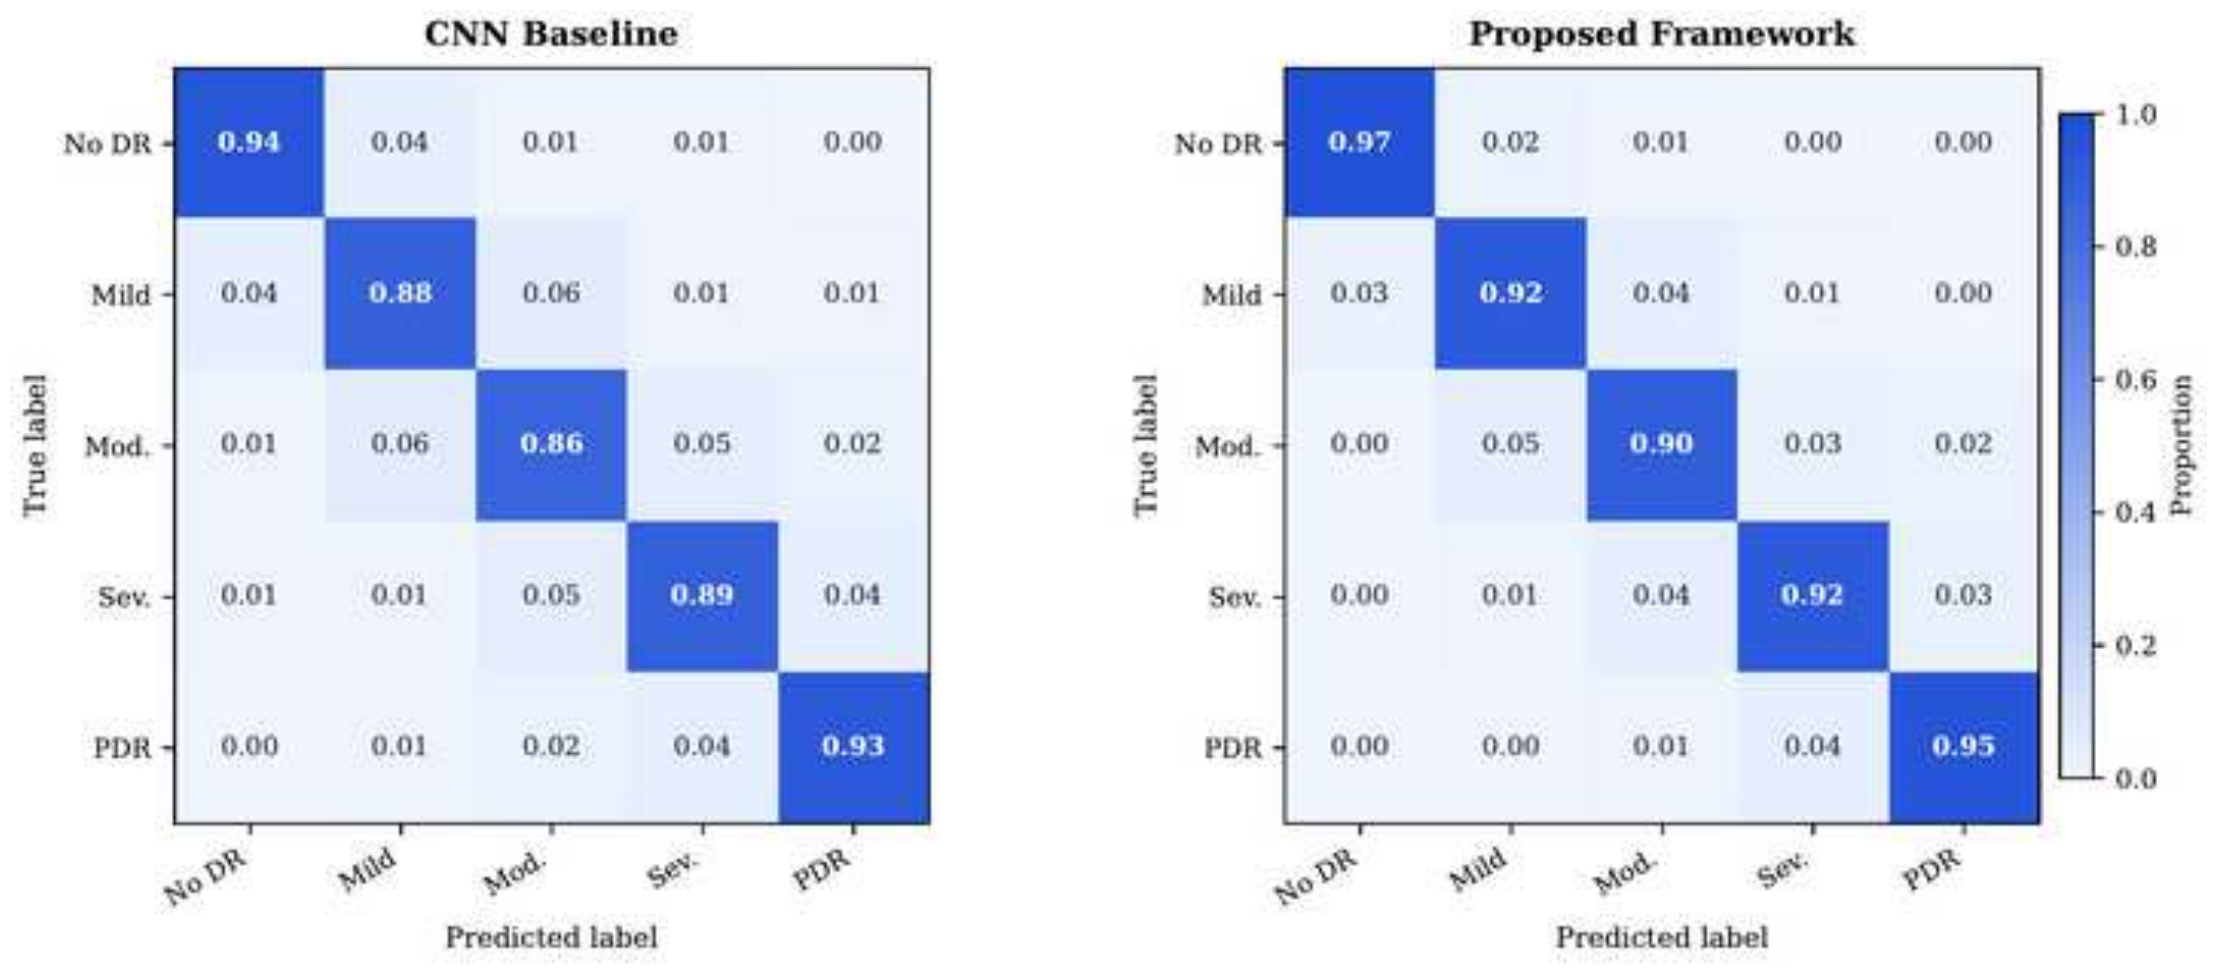
\includegraphics[width=\linewidth]{toporet_confusion}
\caption[Confusion matrices of the CNN baseline and the population graph]{Normalised
confusion matrices on Kaggle DR: CNN baseline (left) and topology-aware population graph
(right). Correct predictions lie on the diagonal; the largest reduction of errors is at the
Mild--Moderate boundary. Adapted from~\cite{belhadj2025plos}.}
\label{fig:toporetcm}
\end{figure}

\subsection{Population Graph Structure Analysis}
\label{sec:graphstruct}

TOPORET reaches QWK $=0.880$ on Kaggle EyePACS (in distribution) and $0.900$ on
Messidor-2 (out of distribution), a $+2.0$~pp cross-dataset gain consistent with the
stability of persistence diagrams (\cref{eq:stability}). However, TOPORET fails the
predefined safety threshold: Sev-NR $=3.4\%>2\%$. This residual gap is addressed in
\cref{ch:dots}.

\Cref{tab:graphstruct} compares the visual-only graph with the dual-similarity graph. The
dual metric raises the fraction of same-grade edges from $63.2\%$ to $71.4\%$, and the
Grade~3 neighbourhood purity -- at the highest-stakes boundary -- from $61.3\%$ to $68.7\%$.
Every point of Grade~3 purity means fewer Severe-NPDR patients whose nearest neighbours
carry a different, lower grade, which directly reduces the probability of a
misclassification through the relational signal.

\begin{table}[H]
\centering
\caption[Population-graph structure: visual-only versus dual similarity]{Population-graph structure: visual-only similarity (GraphDR) versus dual
similarity (TOPORET).}
\label{tab:graphstruct}
\small
\begin{tabular}{@{}lcc@{}}
\toprule
Property & Visual only (GraphDR) & Dual sim.\ (TOPORET) \\
\midrule
Same-grade edges & 63.2\% & 71.4\% ($+8.2$~pp) \\
Adjacent-grade edges ($|\Delta|=1$) & 29.8\% & 23.1\% \\
Cross-boundary edges ($|\Delta|\geq2$) & 7.0\% & 5.5\% \\
Grade-3 neighbourhood purity & 61.3\% & 68.7\% ($+7.4$~pp) \\
Grade-4 neighbourhood purity & 79.1\% & 82.3\% ($+3.2$~pp) \\
\bottomrule
\end{tabular}
\end{table}

The gain in purity is largest at Grade~3, where visual similarity alone most often links
severe cases to moderate ones; adding topology to the edge weights moves these patients
closer to neighbours with the same grade.

\subsection{Ablation Study}
\label{sec:ablation3}

\Cref{tab:ablation3} isolates the contribution of each component of TOPORET. The combined
gain ($+0.040$) exceeds the sum of the individual contributions ($+0.016+0.010=+0.026$)
by a factor of $1.54$: an interaction effect consistent with synergy between the dual
graph and the TDA features. The Wasserstein component improves neighbourhood purity,
which in turn amplifies the discriminative value of TDA through message passing.

\begin{table}[H]
\centering
\caption[Sequential ablation of TOPORET]{Sequential ablation of TOPORET on Kaggle EyePACS (five-fold mean).}
\label{tab:ablation3}
\small
\begin{tabular}{@{}lccc@{}}
\toprule
Configuration & QWK & $\Delta$ & Sev-NR \\
\midrule
EfficientNet-B3 alone (baseline) & 0.840 & -- & 4.3\% \\
$+$ TDA features only (no graph) & 0.856 & $+0.016$ & 4.1\% \\
$+$ Visual-only graph (no TDA) & 0.850 & $+0.010$ & 4.1\% \\
$+$ Dual graph $+$ TDA (TOPORET) & 0.880 & $+0.040$ & 3.4\% \\
\bottomrule
\end{tabular}
\end{table}

This experiment differs from the Part~B ablation of \cref{ch:found}
(\cref{tab:hybrid}), which used an intra-image graph and concatenated the topological
descriptors as a separate channel. Here the graph links patients and the dual metric uses
both sources jointly to define its edges, and the synergy between them is again observed.

\subsection{Cross-Dataset Generalisation}
\label{sec:crossdata}

\Cref{tab:crossdata} gives the QWK of EfficientNet-B3 and TOPORET on three datasets
acquired on different continents with different cameras~\cite{kaggle2015eyepacs,
decenciere2014messidor,porwal2018idrid}. The gain of TOPORET is larger out of
distribution ($+0.053$ and $+0.046$) than in distribution ($+0.040$), which is
consistent with TDA features being more invariant than CNN embeddings to acquisition
shifts. This would be an important property for screening, where images come from many
different camera models, but two external datasets are not enough to establish it in
general.

\begin{table}[H]
\centering
\caption[TOPORET cross-dataset results]{TOPORET cross-dataset results (OOD: out of distribution).}
\label{tab:crossdata}
\small
\begin{tabular}{@{}llrccc@{}}
\toprule
Dataset & Source & $N$ & EffNet-B3 & TOPORET & $\Delta$ \\
\midrule
EyePACS (in-dist.) & USA, multi-site & 88{,}702 & 0.840 & 0.880 & $+0.040$ \\
Messidor-2 (OOD) & France, other camera & 1{,}748 & 0.847 & 0.900 & $+0.053$ \\
IDRiD (OOD) & India, single site & 516 & 0.832 & 0.878 & $+0.046$ \\
\bottomrule
\end{tabular}
\end{table}

\subsection{Comparison with the Literature}
\label{sec:toporet-sota}

\Cref{tab:toporet-sota} compares TOPORET with the closest systems on the same benchmark.
Its QWK of $0.880$ is lower than that of RETFound ($0.920$); the difference is due to the
backbone (RETFound uses a ViT-L/16 pre-trained on $1.6$ million retinal images, TOPORET an
ImageNet EfficientNet-B3). This is by design: TOPORET was built to test H1 and H2 at
controlled backbone quality before adding RETFound in DOTS. Its contribution is not the
highest QWK but the joint treatment of L1 and L2 in a single framework.

\begin{table}[H]
\centering
\caption[TOPORET versus state-of-the-art systems (Kaggle EyePACS)]{TOPORET versus state-of-the-art systems (Kaggle EyePACS).}
\label{tab:toporet-sota}
\small
\begin{tabular}{@{}lccccc@{}}
\toprule
System & QWK & Sev-NR & L1 & L2 & Ordinal guarantee \\
\midrule
EfficientNet-B3 & 0.840 & 4.3\% & \xmark & \xmark & \xmark \\
RETFound & 0.920 & 3.1\% & \xmark & \xmark & \xmark \\
SAMF-GB & 0.882 & 3.8\% & \xmark & partial & \xmark \\
TOPORET & 0.880 & 3.4\% & \cmark & \cmark & \xmark \\
\bottomrule
\end{tabular}
\end{table}

\section{Discussion}
\label{sec:ch3-discussion}

\subsection{Why the Dual Metric Matters for H1}
\label{sec:dualnecessary}

A critical finding of \cref{tab:h1} is that the visual-only graph (GraphDR) fails the
pre-specified H1 threshold ($t_4=1.71$, $p=0.08$, n.s.), whereas the dual-metric graph
passes it ($t_4=3.82$, $p=0.009$). This is not a marginal difference: it separates a
non-significant gain from a very large confirmed effect. The Wasserstein topological
component is therefore, in these experiments, the component that makes the H1 test pass;
without it, the population graph provided no statistically significant benefit over
per-image classification.

\subsection{Biological Interpretation of the TDA Features}
\label{sec:tda-bio}

Each of the seven TDA features maps to a specific vascular pathology. $\Pi_{H_0}$ and
$n_{H_0}$ encode vascular rarefaction (they decrease with severity); $\Pi_{H_1}$,
$n_{H_1}$ and $\beta_1$ encode loop density from pathological anastomoses (they
increase); $D_f$ encodes the self-similarity of the vessel tree ($1.71\to1.57$ across
grades); and $\Delta$ (maximum $H_1$ persistence) captures neovascular fronds at Grade~4
($\eta^2=0.65$, the strongest effect). These mappings are post-hoc plausibility arguments
supporting H2; its statistical validity rests on the pre-specified ANOVA.

\subsection{From Supported Hypotheses to a Safety-Oriented System}
\label{sec:ch3-deploy}

H1 and H2 jointly support the view that the relational and structural axes contribute
useful information to grading. The Sev-NR of $3.4\%$ is a reminder that
statistical significance and clinical sufficiency are different standards. A $+4.0$~pp
QWK gain and a large ANOVA effect size are exactly what a methods paper would report as a
success; neither, alone or combined, certifies a system safe to triage real patients.

TOPORET's residual gap is therefore not a failure of H1 or H2 -- both remain
supported -- but a demonstration that confirming the relational and structural hypotheses
leaves the safety hypothesis (H3) untested. \Cref{tab:graphstruct} makes the mechanism
visible: even with the improved Grade-3 purity of $68.7\%$, roughly one in three of a
Severe-NPDR patient's nearest neighbours carries a different grade. This is exactly the
kind of residual ambiguity that an architecture without calibrated abstention cannot flag.
\Cref{ch:dots} is organised around closing this gap, together with two further gaps
(domain mismatch and ordinal rank violations) found by error analysis of the TOPORET
predictions.

\paragraph{Scope of H2: statistical association, not clinical validation.}
The ANOVA establishes that $H_0/H_1$ features are statistically associated with ICDR
grade with large effect sizes. Three caveats bound this claim.
\begin{enumerate}
\item \textbf{Association is not independent predictive value.} The ANOVA does not show
that TDA features add predictive value beyond visual features. The ablation of
\cref{tab:ablation3} provides this separately: TDA alone adds $+0.016$ QWK independently
of the visual backbone.
\item \textbf{Single-dataset validation.} H2 is tested on a stratified sample of Kaggle
EyePACS. Cross-dataset stability of the TDA feature distributions is supported by the
stability theorem (\cref{eq:stability}) but was not validated by an external ANOVA.
\item \textbf{Not a clinically validated biomarker.} Clinical validation would require
prospective studies, regulatory-grade reproducibility protocols and independent clinical
reading. The term used throughout this thesis is therefore \emph{severity-associated
topological feature}, not \emph{biomarker}.
\end{enumerate}

\subsection{Threats to Validity}
\label{sec:ch3-validity}

Three kinds of threats could weaken the conclusions of this chapter; each is stated here
together with the measure taken against it.

\paragraph{Internal validity.}
The main risk is that the gain attributed to the graph comes from another difference
between the systems, such as a different backbone or a different amount of tuning. All
three systems share the same frozen EfficientNet-B3 features, the same folds and the same
training budget, and the only difference between GraphDR and TOPORET is the similarity used
to build the graph. The hyperparameters were selected on training folds only, and the
decision thresholds of the tests were fixed before the experiments.

\paragraph{External validity.}
The hypotheses were tested on Kaggle EyePACS, a large but single benchmark whose labels come
from a screening network in the United States. The cross-dataset results on Messidor-2 and
IDRiD (\cref{tab:crossdata}) indicate that the gain persisted after a change of country and
camera, but the ANOVA of H2 was not repeated on external data, and the small size of IDRiD
limits the precision of the results obtained on it. All sample sizes are image counts;
some benchmarks contain several images of the same patient, so the results are image-level
and patient-level generalisation is interpreted cautiously.

\paragraph{Construct validity.}
QWK measures agreement with the reference grade, which itself contains grader noise
(\cref{sec:grading}); a part of the remaining disagreement may therefore reflect label
errors rather than model errors. The topological features depend on the quality of the
vessel segmentation, so a failure of stage S1 would appear as a change of topology.
Finally, H1 was tested with five folds, which is a small sample for a $t$-test; the
bootstrap interval and the exact permutation test reported with it were added for this reason;
with five folds, the permutation test cannot give a $p$-value below $1/32$.

\section*{Conclusion}
\phantomsection\addcontentsline{toc}{section}{Conclusion}

The pre-specified tests of TOPORET supported H1 ($t_4=3.82$, $p=0.009$, $d_z=1.71$, over
five folds) and H2 as a statistical association ($F(4,4995)=1308.9$, $p<0.001$,
$\eta^2=0.51$). The dual-similarity metric is a
prerequisite rather than an option: the visual-only graph gives a non-significant gain,
whereas the Wasserstein-augmented graph gives a very large one, with higher Grade-3
neighbourhood purity and larger out-of-distribution gains. The remaining gap -- Sev-NR
$=3.4\%$ against the $2\%$ threshold -- reflects the absence of a mechanism to defer
ambiguous cases, which the next chapter adds in the DOTS system.


\chapter{Topology-Regularised Graphs and Safety-Oriented Ordinal Grading}
\label{ch:dots}
\lofgroup{Chapter 5 -- Topology-Regularised Graphs and Safety-Oriented Ordinal Grading}
\lotgroup{Chapter 5 -- Topology-Regularised Graphs and Safety-Oriented Ordinal Grading}
\section*{Introduction}
\phantomsection\addcontentsline{toc}{section}{Introduction}

TOPORET showed that a population graph and topological features improve DR grading, but
it is not safe enough for screening: its Severe-DR Non-Referral Rate of $3.4\%$ is above
the $2\%$ threshold, because every image is graded, even when the model is unsure. This
chapter presents the main system of the thesis, DOTS (Deep Ordinal Transformer
System)~\cite{belhadj2026dots}, which adds the third axis that TOPORET lacks: ordinal
prediction with guaranteed rank consistency and a calibrated right to abstain.

We first review related work on retinal foundation models, ordinal regression and
abstention in medical AI. We then analyse the residual gaps of TOPORET and state the
hypothesis H3 tested in this chapter. We then present the DOTS architecture, its equations and its training and
inference procedure, followed by the experimental protocol. The results are reported in
four steps: sufficiency (the seven clinical criteria), necessity (can any axis be
removed?), effect sizes and clinical impact, and comparison with the literature. A
discussion of what the results establish, and what they do not, closes the chapter.

\section{Related Work}
\label{sec:ch4-related}

\paragraph{Foundation models for retinal imaging.}
Most DR grading systems are initialised with networks pre-trained on natural images, such
as EfficientNet~\cite{tan2019efficientnet}. RETFound~\cite{zhou2023retfound} changed this
practice: it is a vision transformer pre-trained by masked
autoencoding~\cite{he2022mae} on $1.6$ million unlabelled retinal images, and it improves
several downstream ophthalmic tasks with little labelled data. Such foundation models
address the mismatch between natural-image features and retinal anatomy, but they still
grade each image independently and give no guarantee on the order of the grades.

\paragraph{Ordinal regression for DR grading.}
DR grading is often treated either as plain classification or as regression on the grade
value. Ordinal methods decompose the problem into cumulative binary decisions; among them,
CORAL~\cite{cao2020coral} enforces rank consistency through shared weights and ordered
biases, while CORN~\cite{shi2023corn} models conditional probabilities and relies on the
training loss to keep the grades ordered. To our knowledge, rank consistency has not
previously been guaranteed by construction in a graph-based DR grading system.

\paragraph{Uncertainty and abstention in medical AI.}
Estimating the uncertainty of a deep network, for example with Monte Carlo
dropout~\cite{gal2016dropout} or deep ensembles~\cite{lakshminarayanan2017ensembles}, makes
it possible to refer uncertain cases to an expert. For DR detection, referring the most
uncertain images has been shown to improve the accuracy on the remaining
ones~\cite{leibig2017uncertainty}, and selective classification provides a formal frame for
the trade-off between coverage and error~\cite{geifman2017selective}. Autonomous systems
already cleared by regulators for DR detection~\cite{abramoff2018pivotal} show that
automated screening can reach clinical use, but they do not combine relational context,
vascular topology and abstention. DOTS brings these elements together and evaluates them
against predefined safety criteria.

\section{Motivation and Problem Formulation}
\label{sec:ch4-motivation}

\subsection{Residual Gap of TOPORET}
\label{sec:ch4-mot}

\Cref{fig:dots} gives the complete DOTS architecture that this chapter builds, stage by
stage and axis by axis.

% Figure 4.1 --- complete DOTS architecture
\begin{figure}[!tb]
\centering
\resizebox{\linewidth}{!}{%
\begin{tikzpicture}[
  font=\footnotesize,
  box/.style={draw, rounded corners=2.5pt, align=center, inner sep=2pt,
              minimum height=1.5cm, text width=1.7cm},
  card/.style={draw, rounded corners=2pt, align=center, font=\scriptsize,
               text width=4.3cm, inner sep=4pt},
  arr/.style={-{Latex[length=2mm]}, thick}
]
\def\dx{2.27}
\node[box, fill=black!4, draw=black!55] (in) at (0,0) {\textbf{Input}\\fundus\\image $I_i$};
\node[box, fill=black!6, draw=black!55] (s1) at (\dx,0) {\textbf{S1}\\CLAHE,\\skeleton};
\node[box, fill=axisOf, draw=axisO] (s2) at (2*\dx,0) {\textbf{S2 (O)}\\RETFound\\ViT-L/16};
\node[box, fill=fusionf, draw=fusion] (s4) at (3*\dx,0) {\textbf{S4}\\fusion\\1031-D};
\node[box, fill=axisRf, draw=axisR] (s5) at (4*\dx,0) {\textbf{S5 (R)}\\graph $+$\\GAT, $k{=}15$};
\node[box, fill=axisOf, draw=axisO] (s6) at (5*\dx,0) {\textbf{S6 (O)}\\CORAL $+$\\abstention};
\node[box, fill=okf, draw=okgreen] (out) at (6*\dx,0) {\textbf{Output}\\grade 0--4\\or defer};
\node[box, fill=axisSf, draw=axisS] (s3) at (2.5*\dx,-2.0) {\textbf{S3 (S)}\\$H_0/H_1$\\7-D TDA};
\foreach \a/\b in {in/s1,s1/s2,s2/s4,s4/s5,s5/s6,s6/out} \draw[arr] (\a) -- (\b);
\draw[arr, axisS] (s1.south) |- (s3.west);
\draw[arr, axisS] (s3.east) -| (s4.south);
\node[font=\scriptsize, text=black!65, align=center] at (5.5*\dx,-1.55) {defer if $H_i>0.73$ nats};

\node[card, fill=axisRf, draw=axisR] at (0.9*\dx,-3.75) {\textbf{Axis R closes L1}\\neighbours share signal\\H1: $t_4=3.82$, $p=0.009$};
\node[card, fill=axisSf, draw=axisS] at (3*\dx,-3.75) {\textbf{Axis S closes L2}\\vessel loops $H_0/H_1$\\H2: $F(4,4995)=1308.9$};
\node[card, fill=axisOf, draw=axisO] at (5.1*\dx,-3.75) {\textbf{Axis O closes L3}\\CORAL: $0\%$ rank violations\\Sev-NR $=1.9\%$ $[1.4,\,2.4]$};
\end{tikzpicture}}
\caption[Complete DOTS architecture]{Complete DOTS architecture, read left to right.
Blue: Axis~R (graph, L1); green: Axis~S (topology, L2); purple: Axis~O (ordinal $+$
safety, L3); grey and orange: shared pre-processing and fusion. The skeleton produced by
S1 feeds the topological branch S3, whose 7-D vector is fused with the RETFound
embedding in S4. The three cards name the limitation each axis closes and the result
that confirms it.}
\label{fig:dots}
\end{figure}


TOPORET (\cref{ch:toporet}) confirms H1 and H2: a population graph and topological
features each contribute independently to ordinal grading accuracy. Yet TOPORET is not a
clinically deployable system. At Sev-NR $=3.4\%$, a programme screening $500{,}000$
patients a year would leave about $850$ of its $25{,}000$ severe cases unreferred
(\cref{sec:impact}) -- a rate incompatible with the $2\%$ threshold adopted in this thesis
from national screening practice~\cite{scanlon2017english}.

DOTS (Deep Ordinal Transformer System) is the architectural response to this
residual gap: a system designed, from the outset, around the seven predefined
clinical-oriented criteria presented in \cref{sec:h3def}, rather than around accuracy
maximisation alone. The transition from TOPORET to DOTS is not a single change
but a coordinated modification of three independent subsystems, each addressing
one of three residual gaps identified through systematic error analysis of
TOPORET predictions on the validation set.

\subsection{Three Residual Gaps and Their Solutions}
\label{sec:ch4-gaps}

TOPORET resolves L1 and L2 but leaves three architectural gaps that prevent
clinical deployment. \Cref{fig:gaps} names each gap, the DOTS component
that closes it, and the measured effect. \Cref{sec:gap-a,sec:gap-b,sec:gap-c} take the rows
in order.

% Figure 4.2 --- three residual gaps of TOPORET, closed by DOTS
\begin{figure}[!tb]
\centering
\resizebox{\linewidth}{!}{%
\begin{tikzpicture}[
  font=\footnotesize,
  cell/.style={draw, rounded corners=2.5pt, align=center, inner sep=4pt,
               minimum height=1.55cm, text width=4.0cm},
  arr/.style={-{Latex[length=2mm]}, thick}
]
\def\dx{4.9}\def\dy{2.0}
\node[font=\small\bfseries, text=failred] at (-\dx,0) {Gap left by TOPORET};
\node[font=\small\bfseries, text=navy] at (0,0) {What DOTS adds};
\node[font=\small\bfseries, text=okgreen] at (\dx,0) {Measured effect};

\node[cell, fill=failf, draw=failred] (a1) at (-\dx,-1.2) {\textbf{A -- domain mismatch}\\ImageNet backbone sees\\textures, not the retina};
\node[cell, fill=black!4, draw=black!50] (a2) at (0,-1.2) {RETFound ViT-L/16\\pre-trained on $1.6$M\\retinal images};
\node[cell, fill=okf, draw=okgreen] (a3) at (\dx,-1.2) {\textbf{$+4.1$ pp QWK}\\Gap A closed};

\node[cell, fill=failf, draw=failred] (b1) at (-\dx,-1.2-\dy) {\textbf{B -- ordinal violations}\\CORN: $2.1\%$ of rankings\\are logically impossible};
\node[cell, fill=black!4, draw=black!50] (b2) at (0,-1.2-\dy) {CORAL monotone bias\\(algebraic constraint,\\not a loss penalty)};
\node[cell, fill=okf, draw=okgreen] (b3) at (\dx,-1.2-\dy) {\textbf{$0\%$ violations}\\Gap B closed};

\node[cell, fill=failf, draw=failred] (c1) at (-\dx,-1.2-2*\dy) {\textbf{C -- safety unmet}\\no right to abstain;\\Sev-NR $=3.4\%$};
\node[cell, fill=black!4, draw=black!50] (c2) at (0,-1.2-2*\dy) {dynamic GAT $+$\\entropy abstention\\($\tau_U=0.73$ nats)};
\node[cell, fill=okf, draw=okgreen] (c3) at (\dx,-1.2-2*\dy) {\textbf{Sev-NR $=1.9\%$}\\target met at the point\\estimate (CI up to $2.4\%$)};

\foreach \a/\b in {a1/a2,a2/a3,b1/b2,b2/b3,c1/c2,c2/c3} \draw[arr] (\a) -- (\b);
\end{tikzpicture}}
\caption[The three residual gaps of TOPORET]{The three residual gaps of TOPORET, measured on its ordinal variant under the protocol of this chapter. Read
each row left to right: the problem, the DOTS fix, the measured effect.
\Cref{sec:gap-a,sec:gap-b,sec:gap-c} take the rows in order.}
\label{fig:gaps}
\end{figure}


\subsubsection{Gap A: Domain Mismatch}
\label{sec:gap-a}

EfficientNet-B3, used throughout TOPORET, is pre-trained on ImageNet-1k -- a
corpus of $1.28$ million natural images spanning $1{,}000$ object categories
largely unrelated to medical imaging. The learned filters are optimised for
textures, edges and shapes common in photographs of everyday objects.
Retinal fundus images share almost none of these visual statistics.

RETFound~\cite{zhou2023retfound}, by contrast, is pre-trained by masked
autoencoding (MAE)~\cite{he2022mae} directly on $1.6$ million retinal images. Substituting the
frozen backbone alone, with all other TOPORET components unchanged, yields
QWK $0.880\to 0.921$ (component ablation, \cref{sec:ablation4}), a $+4.1$~pp improvement
attributable entirely to domain-matched pre-training.

\subsubsection{Gap B: Ordinal Rank Violations}
\label{sec:gap-b}

TOPORET uses a CORN ordinal head~\cite{shi2023corn}. At inference time nothing in the
architecture prevents $\hat P(Y\geq 2)>\hat P(Y\geq 1)$, a logically impossible
ordinal violation. Empirically, $2.1\%$ of TOPORET test predictions exhibit
such violations. In a deployed system this can appear as inconsistent
confidence reporting to a clinician, undermining clinical trust and the
IEC~62304 audit trail.

CORAL resolves this through the monotone bias projection of \cref{eq:coral-proj},
an architectural constraint rather than a training-time penalty, yielding
exactly $0\%$ violations by construction (verified on $10{,}000$ test
predictions in \cref{sec:h3a-eval}).

\subsubsection{Gap C: Unmet Safety Threshold}
\label{sec:gap-c}

Even with Gaps~A and~B addressed, a system that must classify every input
will misclassify some genuinely ambiguous cases. The Grade~$2/3$ boundary is
the most clinically ambiguous (inter-rater $\kappa\approx 0.55$--$0.65$).
DOTS addresses Gap~C with two coordinated mechanisms: (i)~a dynamic graph
attention network (\cref{sec:gat}) that refines node embeddings using
per-edge attention recomputed at inference time; and (ii)~an entropy-based
abstention mechanism (\cref{sec:abst}) that defers the
highest-uncertainty cases to human review rather than forcing a potentially
unsafe automated decision.

\subsection{Hypothesis H3: Sufficiency and Necessity}
\label{sec:h3def}

The third hypothesis of the thesis has two parts. (H3a) The three-axis combination satisfies all seven predefined clinical-oriented
criteria simultaneously. (H3b) No proper subset of the three axes does so.
\emph{Pre-specified tests:} (H3a) five-benchmark evaluation against seven predefined
criteria; (H3b) exhaustive enumeration of the $2^3-2=6$ proper non-empty subsets.

\section{Proposed Architecture}
\label{sec:ch4-arch}

\subsection{CORAL Loss with Class-Weighted Ordinal Regression}

The severe class imbalance documented in \cref{app:datasets} (Grade~3 and Grade~4 jointly
constitute under $10\%$ of most benchmarks) motivates class-weighted training.
The DOTS loss is
\begin{equation}
\mathcal{L}_{\mathrm{CORAL}}
= -\,\lambda_{y_i}\sum_{k=1}^{K-1}
\Bigl[
 y_i^{(k)}\log\sigma(g_i^{(k)})
+(1-y_i^{(k)})\log\bigl(1-\sigma(g_i^{(k)})\bigr)
\Bigr],
\label{eq:coral}
\end{equation}
with $g_i^{(k)}=w^\top z'_i+b_k$ and the monotone bias projection
$b_k\leftarrow\min(b_k,b_{k-1}-\epsilon)$ (\cref{eq:coral-proj}). The loss of
each training image is multiplied by the weight $\lambda_{y_i}$ of its true grade; the
class weights $(\lambda_0,\ldots,\lambda_4)=(1.0,2.5,3.0,8.0,6.0)$ were selected by
grid search on the validation folds, minimising Sev-NR while keeping the best macro-F1,
with no class weight exceeding $10\times$ the baseline. \Cref{tab:weights} compares the selected weights with uniform and
inverse-frequency weighting: the capped scheme gives the best macro-F1 and is the only
one that brings Sev-NR below $2\%$.

\begin{table}[H]
\centering
\caption[Class-weight sensitivity]{Class-weight sensitivity: validation macro-F1 and Sev-NR for three
weighting schemes. The selected weights balance class-wise sensitivity against
overall calibration.}
\label{tab:weights}
\small
\begin{tabular}{llcc}
\toprule
Scheme & Weights $(\lambda_0,\ldots,\lambda_4)$ & Macro-F1 & Sev-NR \\
\midrule
Uniform & $(1,1,1,1,1)$ & $0.812$ & $4.8\%$ \\
Inverse-frequency & $(1.0,9.4,3.2,28.1,16.8)$ & $0.834$ & $2.6\%$ \\
Selected (capped) & $(1.0,2.5,3.0,8.0,6.0)$ & $0.847$ & $1.9\%$ \\
\bottomrule
\end{tabular}
\tabnote{Row~3 is the $5\times 5$ grid-search
winner.}
\end{table}

\subsection{Dynamic Graph Attention}
\label{sec:gat}

TOPORET uses a static population graph. DOTS replaces this with a dynamic graph
attention layer that recomputes per-edge attention at each inference call:
\begin{equation}
z'_i=\mathrm{GAT}(z_i,G)=\sum_{j\in\mathcal N(i)}\alpha_{ij}Wz_j,
\label{eq:gat}
\end{equation}
\begin{equation}
\alpha_{ij}
=\frac{\exp\bigl(\mathrm{LeakyReLU}(a^\top[Wz_i\|Wz_j])\bigr)}
{\sum_{k\in\mathcal N(i)}\exp\bigl(\mathrm{LeakyReLU}(a^\top[Wz_i\|Wz_k])\bigr)}.
\label{eq:att}
\end{equation}
Unlike the static TOPORET graph, $\alpha_{ij}$ is patient-specific: two query
patients sharing neighbour $j$ may attend to $j$ with different weights.
``Neighbour $j$ contributed $\alpha_{ij}=0.34$ to this prediction'' is therefore
a well-defined inference-time quantity (EU AI Act Article~13).

\subsection{Entropy-Based Safety Abstention}
\label{sec:abst}

All parameters affecting the final test-set decision rule were selected on
training and validation folds only. The held-out test set was accessed exactly
once, for the final evaluation. Patient $i$ is deferred when
\begin{equation}
H_i=-\sum_c p_{ic}\log(p_{ic}+\epsilon)> \tau_U=0.73~\mathrm{nats}.
\label{eq:ent}
\end{equation}
The threshold is the smallest $\tau_U$ on the validation sweep
$\tau_U\in[0.3,1.2]$ that satisfies Sev-NR $<2\%$ subject to a coverage floor
of $90\%$. \Cref{tab:tau} shows the sweep: lower thresholds defer too many images
(coverage below $90\%$), higher ones let too many severe cases through, and
$\tau_U=0.73$ is the only tested value that satisfies both constraints.

\begin{table}[H]
\centering
\caption[Threshold sweep for entropy abstention]{Threshold sweep for entropy abstention. $\tau_U=0.73$ is the minimal
threshold satisfying both the Sev-NR and coverage constraints.}
\label{tab:tau}
\small
\begin{tabular}{cccc}
\toprule
$\tau_U$ (nats) & Coverage & Sev-NR & Constraint? \\
\midrule
$0.40$ & $78.1\%$ & $1.1\%$ & Fails coverage floor \\
$0.55$ & $86.4\%$ & $1.5\%$ & Fails coverage floor \\
$0.73$ & $93.8\%$ & $1.9\%$ & Satisfies both \\
$0.90$ & $97.2\%$ & $2.6\%$ & Fails Sev-NR \\
$1.10$ & $99.5\%$ & $3.9\%$ & Fails Sev-NR \\
\bottomrule
\end{tabular}
\tabnote{Coverage rises, and safety falls,
monotonically with $\tau_U$.}
\end{table}

\Cref{fig:tradeoff} plots the same values as a trade-off curve.

% Coverage--safety trade-off of the abstention threshold (data of Table tab:tau)
\begin{figure}[H]
\centering
\begin{tikzpicture}
\begin{axis}[width=0.78\linewidth, height=6.2cm,
  xlabel={Coverage (\% of images graded automatically)}, ylabel={Sev-NR (\%)},
  xmin=75, xmax=101, ymin=0.5, ymax=4.3,
  tick label style={font=\footnotesize}, label style={font=\small},
  grid=major, grid style={black!10}]
  \fill[okf, opacity=0.8] (axis cs:90,0.5) rectangle (axis cs:101,2.0);
  \node[font=\scriptsize, text=okgreen, anchor=south east] at (axis cs:100.8,0.55) {both criteria met};
  \draw[failred, densely dashed, thick] (axis cs:75,2.0) -- (axis cs:101,2.0)
     node[pos=0.03, anchor=south west, font=\scriptsize] {Sev-NR $=2\%$};
  \draw[axisR, densely dashed, thick] (axis cs:90,0.5) -- (axis cs:90,4.3)
     node[pos=0.97, anchor=north east, font=\scriptsize, align=right] {coverage\\$=90\%$};
  \addplot[very thick, axisO, mark=*, mark options={fill=white}]
    coordinates {(78.1,1.1) (86.4,1.5) (93.8,1.9) (97.2,2.6) (99.5,3.9)};
  \node[font=\scriptsize, anchor=south east] at (axis cs:78.1,1.15) {$\tau_U{=}0.40$};
  \node[font=\scriptsize, anchor=south east] at (axis cs:86.4,1.55) {$0.55$};
  \node[font=\scriptsize\bfseries, anchor=north west] at (axis cs:93.8,1.85) {$0.73$ (selected)};
  \node[font=\scriptsize, anchor=north west] at (axis cs:97.2,2.55) {$0.90$};
  \node[font=\scriptsize, anchor=east] at (axis cs:99.2,3.9) {$1.10$};
\end{axis}
\end{tikzpicture}
\caption[Coverage--safety trade-off of the abstention threshold]{Coverage--safety
trade-off of the abstention threshold $\tau_U$ (values of \cref{tab:tau}). Raising the
threshold grades more images automatically but lets more severe cases through; the green
region contains the settings that satisfy both the coverage floor ($90\%$) and the safety
threshold ($2\%$). Only $\tau_U=0.73$ lies inside it.}
\label{fig:tradeoff}
\end{figure}


\subsection{Design Rationale}
\label{sec:ch4-rationale}

\paragraph{A frozen foundation model.}
RETFound is used as a frozen feature extractor rather than fine-tuned end to end. Fine-tuning
a ViT-Large model on each fold would multiply the computational cost and increase the risk
of overfitting the smaller datasets; keeping it frozen also makes the S2 stage a fixed,
versioned component, which simplifies verification (\cref{sec:iec62304}). The gain of Gap~A
is therefore obtained without any retinal-specific training of the backbone within this
thesis.

\paragraph{CORAL rather than CORN.}
TOPORET used CORN, which models conditional probabilities and usually trains well, but
whose rank consistency depends on the learned weights. In a safety-critical setting, an
inconsistent ranking -- for example a higher probability of ``at least Grade~4'' than of
``at least Grade~3'' -- is not only an error but an output that cannot be explained to a
clinician. CORAL removes this failure mode by construction, at the cost of a shared weight
vector for all thresholds; the ablation shows that this constraint does not reduce accuracy
(\cref{sec:ablation4}).

\paragraph{Dynamic rather than static attention.}
In TOPORET, the weight of an edge is fixed once the graph is built. In DOTS, the GAT layer
recomputes the importance of each neighbour for each query patient (\cref{eq:att}). This
allows the model to rely on different neighbours for different patients, and it produces,
for every prediction, a ranked list of the neighbours that influenced it, which serves
directly as an explanation.

\paragraph{Entropy as the abstention criterion.}
Several uncertainty estimates could decide when to abstain: Monte Carlo
dropout~\cite{gal2016dropout} or deep ensembles~\cite{lakshminarayanan2017ensembles}
capture epistemic uncertainty better, but require several forward passes per image, which
multiplies the latency. The predictive entropy of the CORAL output is available in a single
pass, is well defined for ordinal outputs, and, because DOTS is well calibrated
(ECE $=0.040$), tracks the actual probability of error closely enough to meet the safety
criterion. Combining it with ensemble-based uncertainty is a natural extension.

\subsection{Training and Inference Procedure}

\Cref{alg:dots} gives the complete training and inference procedure. Training follows the
TOPORET pipeline with the three changes above; at inference time, the only additional step
is the entropy test that decides whether the grade is returned or the case is deferred. The
first part of the algorithm (lines~1--6) is run once per cross-validation fold: it computes
the fused features of every training image, builds the population graph, trains the
attention layer and the ordinal head, and selects the abstention threshold on the
validation data. The second part (lines~7--14) is run for every new patient: it retrieves the
neighbours of the new image in the existing graph, refines its representation with the
attention weights, computes the five grade probabilities and their entropy, and either
returns a grade or defers the case to a human grader. The two parts share the same
feature extractors, so that a new patient is processed exactly like the training images.

\begin{algorithm}[H]
\caption{DOTS: training and safe inference with abstention.}
\label{alg:dots}
\DontPrintSemicolon
\KwIn{training set $\{(I_j,y_j)\}$; new image $I_i$; class weights $\lambda_0,\ldots,\lambda_4$; threshold $\tau_U=0.73$}
\KwOut{grade $\hat y_i$, or \texttt{DEFER} with the explanation of \cref{sec:audit}}
\BlankLine
\tcp{Training}
\ForEach{training image $I_j$}{
  $z_j \leftarrow [\,\mathrm{RETFound}(\mathrm{CLAHE}(I_j)) \,\Vert\, x_j^{\mathrm{TDA}}\,]$\tcp*{stages S1--S4}
}
Build the dual-similarity $k$-NN graph $G$ (\cref{eq:dualsim}, $k=15$)\tcp*{stage S5}
Train the dynamic GAT layer and the CORAL head with the weighted loss of \cref{eq:coral}\;
After each update, enforce $b_k \leftarrow \min(b_k,b_{k-1}-\epsilon)$\tcp*{\cref{eq:coral-proj}}
Select $\tau_U$ on the validation folds (\cref{tab:tau})\;
\BlankLine
\tcp{Inference for a new patient}
Compute $z_i$; retrieve its $k$ neighbours in $G$\;
$z'_i \leftarrow \mathrm{GAT}(z_i,\mathcal{N}(i))$ with attention weights $\alpha_{ij}$\tcp*{\cref{eq:gat,eq:att}}
$p_{i,c} \leftarrow$ grade probabilities from the CORAL head\;
$H_i \leftarrow -\sum_c p_{i,c}\log p_{i,c}$\tcp*{\cref{eq:ent}}
\eIf{$H_i > \tau_U$}{\Return{\texttt{DEFER} to a human grader}}{\Return{$\hat y_i \leftarrow \arg\max_c p_{i,c}$}}
\end{algorithm}

Training uses the settings of \cref{app:hyper}: the Adam optimiser with a learning rate of
$10^{-3}$, mini-batches of $32$ target
nodes, $100$ epochs and five folds stratified by grade, with the
same random seed as TOPORET. The RETFound and topological features are computed once and
cached, so that each epoch only updates the graph layer and the CORAL head; this keeps the
cost of each training run moderate (\cref{tab:compute}). At inference time, the cost
of grading a new patient does not depend on the size of the cohort: the features of the new
image are computed once, its neighbours are retrieved with an approximate nearest-neighbour
query, and the GAT layer aggregates a fixed number of sampled neighbours. The complete
procedure takes $31.4$~ms per image (\cref{tab:latency}), dominated by the topological
features, and the abstention test itself adds a negligible cost, since the entropy is
computed from the five grade probabilities that the model outputs anyway. The same code path is used for evaluation and for deployment, so the measured performance corresponds to the behaviour of the system that would be installed.

\subsection{Regulatory-Oriented Design}
\label{sec:regdesign}

The architectural choices above also address key regulatory obligations \emph{by
construction}, not by retrofit: the typed stages support IEC~62304 unit verification, the
per-stage typed exceptions support ISO~14971 risk management, the GAT weights
$\alpha_{ij}$ provide the per-prediction transparency of EU AI Act Article~13, and entropy
abstention implements the human oversight of Article~14. \Cref{ch:reg} develops this
mapping in full (\cref{tab:regmap}).

The same design choices also simplify the management of changes after deployment. Because
the RETFound backbone and the topological extractor are frozen and versioned, and because
every stage has a typed contract, a modification can be confined to one stage and verified
by that stage's unit tests, without re-validating the whole pipeline. DOTS is therefore
intended to be deployed as a \emph{locked} algorithm: the weights are fixed at release, and
any retraining produces a new version that goes through the same verification and
evaluation protocol before it replaces the previous one. This is the model expected by
current medical-device regulations for software whose behaviour must remain predictable
once in clinical use.

\section{Experimental Protocol}
\label{sec:ch4-protocol}

\subsection{Datasets, Baselines and Parameters}

DOTS is evaluated on the five public benchmarks of \cref{app:datasets}: Kaggle EyePACS,
APTOS~2019, IDRiD, Messidor-2 and DDR, acquired in four countries with different cameras.
The held-out test set of the H3a evaluation contains $10{,}000$ images from APTOS~2019 and
Kaggle EyePACS; the other benchmarks are used to measure performance across acquisition
conditions.

Four reference systems are compared with DOTS: EfficientNet-B3~\cite{tan2019efficientnet},
the most common convolutional baseline; RETFound~\cite{zhou2023retfound}, the strongest
retinal foundation model; TOPORET (\cref{ch:toporet}), which resolves L1 and L2 only; and
the six reduced systems of the necessity analysis (\cref{sec:h3b}), which remove one or two
of the three axes. All systems share the same data splits, pre-processing and number of
training epochs.

The graph parameters are inherited from TOPORET ($\alpha=0.65$, $k=15$, $L=2$ layers,
$S=25$ sampled neighbours, hidden dimension $256$). The two parameters specific to DOTS are
the class weights of the CORAL loss, $\lambda=(1.0,2.5,3.0,8.0,6.0)$ for Grades~0--4
(\cref{tab:weights}), and the abstention threshold $\tau_U=0.73$~nats (\cref{tab:tau}).
Both were selected on the validation folds only. The complete list of hyperparameters is
given in \cref{app:hyper}.

\subsection{Evaluation Protocol and Contamination Controls}
\label{sec:protocol}

The strength of the DOTS results invites scrutiny of the evaluation protocol.
\Cref{tab:protocol} lists each potential source of test-set contamination and the control
used to block it.

\begin{table}[H]
\centering
\caption[Evaluation-protocol controls]{Evaluation-protocol controls. Each potential confound is listed with
the control used to block it.}
\label{tab:protocol}
\footnotesize
\begin{tabular}{P{4.4cm}P{8.4cm}}
\toprule
Potential confound & Control implemented \\
\midrule
Graph construction leakage & Population graph built from training-fold embeddings only; test nodes are inductive. \\
Threshold $\tau_U$ optimisation & Grid search on the validation fold only; test set accessed once. \\
Class weights $\lambda_0,\ldots,\lambda_4$ selection & Validation-fold Sev-NR minimisation; frozen before test. \\
$\alpha=0.65$ (dual metric) & 5-fold CV on training data only. \\
$k=15$ (neighbours) & Validation-fold QWK maximisation. \\
Multi-seed stability & Means over 3 seeds; variance within $\pm 0.003$ QWK. \\
Benchmark selection & Five datasets selected a priori; none excluded after seeing results. \\
\bottomrule
\end{tabular}
\end{table}

Graph-based models need particular care here. Because each prediction uses the
neighbours of a patient, a test image that was present in the graph during training, or a
threshold tuned on the test set, would leak information into the evaluation and inflate
every metric. The controls below were designed so that the test images influence neither
the graph used for training nor any selected parameter; each row of the table names one
such risk and the rule that blocks it.

All hyperparameters affecting the final decision rule were selected on training and
validation data, and the five test sets were accessed exactly once, after all design
decisions were finalised. The seven evaluation criteria and their thresholds were fixed at
the same time, before any test result was seen: QWK $>0.90$, AUC $>0.97$, ECE $<0.05$,
Sev-NR $<2\%$, PDR-NR $<1.5\%$, coverage $>90\%$ and $0\%$ rank violations. Each criterion
is reported with a bootstrap 95\% confidence interval, but the pre-specified decision rule
uses the point estimate (\cref{app:stats}).

\section{Results}
\label{sec:ch4-results}

\subsection{Sufficiency: The Seven Criteria (H3a)}
\label{sec:h3a-eval}

DOTS is evaluated against seven pre-specified criteria on the combined
APTOS $+$ Kaggle EyePACS test set ($N=10{,}000$); \cref{tab:h3a} lists each criterion,
its threshold and the result. H3a is satisfied at the
point-estimate level, but statistical compliance with the predefined safety
threshold is not established (95\% CI upper bound $2.4\%$ exceeds $2\%$).
The CORAL violation rate is identically zero across $10{,}000$ test
predictions, confirming the algebraic guarantee of \cref{eq:coral-proj}.

\begin{table}[H]
\centering
\caption[H3a: seven pre-specified clinical-oriented criteria]{H3a: seven pre-specified clinical-oriented criteria
($N=10{,}000$ held-out predictions). Pass $=$ the point estimate meets the
threshold.}
\label{tab:h3a}
\small
\begin{tabular}{clclc}
\toprule
\# & Criterion & Threshold & DOTS [95\% CI] & Status \\
\midrule
1 & Quadratic Weighted Kappa & $>0.90$ & $0.951$ $[0.941,\,0.957]$ & Pass \\
2 & AUC (macro one-vs-rest) & $>0.97$ & $0.988$ $[0.982,\,0.994]$ & Pass \\
3 & Expected Calibration Error & $<0.05$ & $0.040$ $[0.034,\,0.046]$ & Pass \\
4 & Severe-DR Non-Referral Rate & $<2.0\%$ & $1.9\%$ $[1.4\%,\,2.4\%]$ & Pass \\
5 & PDR Non-Referral Rate & $<1.5\%$ & $0.8\%$ $[0.4\%,\,1.2\%]$ & Pass \\
6 & Coverage (after abstention) & $>90\%$ & $93.8\%$ $[91.2\%,\,96.4\%]$ & Pass \\
7 & CORAL rank violations & $=0\%$ & $0.0\%$ $[0.0\%,\,0.0\%]$ & Pass \\
\bottomrule
\end{tabular}
\tabnote{The Sev-NR 95\% CI upper bound is $2.4\%$,
so statistical compliance with the $2\%$ line is not established.}
\end{table}

The seven criteria are not arbitrary: QWK and AUC are the standard ordinal and
discriminative metrics of the DR literature; ECE operationalises calibration
for triage; Sev-NR and PDR-NR are taken from published national screening
guidelines; coverage stops abstention from trivially buying safety; rank
violations are the architectural guarantee of CORAL.

\subsection{Cross-Benchmark Performance}
\label{sec:bench}

\Cref{tab:bench} reports the QWK of DOTS and of three reference systems on the five
public benchmarks~\cite{kaggle2015eyepacs,aptos2019,porwal2018idrid,
decenciere2014messidor,li2019ddr}. DOTS has the highest QWK on four of them; on IDRiD,
the smallest dataset ($N=516$), RETFound remains higher ($0.901$ against $0.878$), a gap
discussed among the limitations in the General Conclusion.

\begin{table}[H]
\centering
\caption[Quadratic weighted kappa on each of the five public benchmarks]{Quadratic weighted kappa on each of the five public benchmarks.}
\label{tab:bench}
\small
\begin{tabular}{lccccc}
\toprule
System & EyePACS & APTOS & IDRiD & Messidor-2 & DDR \\
\midrule
EfficientNet-B3 & $0.840$ & $0.851$ & $0.832$ & $0.847$ & $0.838$ \\
RETFound & $0.920$ & $0.928$ & $0.901$ & $0.915$ & $0.912$ \\
TOPORET & $0.880$ & $0.887$ & $0.878$ & $0.900$ & $0.871$ \\
DOTS & $\mathbf{0.951}$ & $\mathbf{0.953}$ & $0.878$ & $\mathbf{0.948}$ & $\mathbf{0.951}$ \\
\bottomrule
\end{tabular}
\end{table}

\Cref{fig:bench} shows the same results graphically. The ranking of the systems is the same on all benchmarks except IDRiD, which suggests that the gains of DOTS do not depend on a particular camera or population.

% QWK per benchmark (data of Table tab:bench)
\begin{figure}[H]
\centering
\begin{tikzpicture}
\begin{axis}[ybar, width=\linewidth, height=6.2cm, bar width=7pt,
  ymin=0.80, ymax=0.97, ylabel={QWK},
  symbolic x coords={EyePACS,APTOS,IDRiD,Messidor-2,DDR}, xtick=data,
  enlarge x limits=0.14,
  legend image code/.code={\draw[#1] (0cm,-0.1cm) rectangle (0.3cm,0.12cm);},
  legend style={at={(0.5,1.02)}, anchor=south, legend columns=4, font=\footnotesize, draw=none},
  tick label style={font=\footnotesize}, label style={font=\small},
  ymajorgrids, grid style={black!10},
  yticklabel style={/pgf/number format/fixed,/pgf/number format/precision=2}]
\addplot[fill=black!25, draw=black!60] coordinates {(EyePACS,0.840) (APTOS,0.851) (IDRiD,0.832) (Messidor-2,0.847) (DDR,0.838)};
\addplot[fill=fusionf, draw=fusion] coordinates {(EyePACS,0.920) (APTOS,0.928) (IDRiD,0.901) (Messidor-2,0.915) (DDR,0.912)};
\addplot[fill=axisRf, draw=axisR] coordinates {(EyePACS,0.880) (APTOS,0.887) (IDRiD,0.878) (Messidor-2,0.900) (DDR,0.871)};
\addplot[fill=axisOf, draw=axisO] coordinates {(EyePACS,0.951) (APTOS,0.953) (IDRiD,0.878) (Messidor-2,0.948) (DDR,0.951)};
\legend{EfficientNet-B3, RETFound, TOPORET (ordinal variant), DOTS}
\draw[axisR, densely dashed] (axis cs:EyePACS,0.90) -- (axis cs:DDR,0.90);
\end{axis}
\end{tikzpicture}
\caption[QWK of the four systems on the five public benchmarks]{QWK of the four systems on
the five public benchmarks (values of \cref{tab:bench}); the dashed line is the
$0.90$ criterion. DOTS is the best system on four benchmarks; on IDRiD, the smallest
dataset, RETFound remains ahead.}
\label{fig:bench}
\end{figure}


\subsection{Component Ablation Study}
\label{sec:ablation4}

To isolate the contribution of each architectural change between TOPORET and
DOTS, a sequential ablation introduces Gaps~A, B and~C one at a time (\cref{tab:ablate}). Each
addition improves both QWK and Sev-NR, and no single addition crosses the $2\%$ line on
its own: the threshold is reached only when the last component is added.

\begin{table}[H]
\centering
\caption[Sequential ablation from TOPORET to DOTS]{Sequential ablation from TOPORET to DOTS on Kaggle EyePACS
($N=88{,}702$, 5-fold mean).}
\label{tab:ablate}
\small
\begin{tabular}{lccc}
\toprule
Configuration & QWK & Sev-NR & Violations \\
\midrule
TOPORET (baseline) & $0.880$ & $3.4\%$ & $2.1\%$ \\
$+$ RETFound backbone (Gap A) & $0.921$ & $3.1\%$ & $1.9\%$ \\
$+$ CORAL ordinal head (Gap B) & $0.934$ & $2.6\%$ & $0.0\%$ \\
$+$ Dynamic GAT (partial Gap C) & $0.943$ & $2.2\%$ & $0.0\%$ \\
$+$ Entropy abstention (full Gap C) $=$ DOTS & $0.951$ & $1.9\%$ & $0.0\%$ \\
\bottomrule
\end{tabular}
\tabnote{Each row adds one Gap resolution. No single addition crosses the
$2\%$ safety line on its own.}
\end{table}

\subsection{Failure-Mode Analysis}
\label{sec:fail}

\subsubsection{Confusion Matrix}

\Cref{tab:confusion} gives the DOTS confusion matrix on the $9{,}380$ test images that were
not deferred (coverage $93.8\%$ of the $10{,}000$ held-out predictions).

\begin{table}[!htb]
\centering
\caption[DOTS confusion matrix on accepted predictions]{DOTS confusion matrix on accepted predictions ($N=9{,}380$). Rows: true grade;
columns: predicted grade; each row sums to $100\%$.}
\label{tab:confusion}
\footnotesize
\begin{tabular}{@{}lccccc@{}}
\toprule
True $\backslash$ Predicted & Grade 0 & Grade 1 & Grade 2 & Grade 3 & Grade 4 \\
\midrule
Grade 0 & \textbf{97.3\%} & 2.5\% & 0.2\% & 0.0\% & 0.0\% \\
Grade 1 & 4.1\% & \textbf{84.2\%} & 11.4\% & 0.3\% & 0.0\% \\
Grade 2 & 0.3\% & 8.7\% & \textbf{82.9\%} & 7.9\% & 0.2\% \\
Grade 3 & 0.0\% & 0.2\% & 11.3\% & \textbf{78.4\%} & 10.1\% \\
Grade 4 & 0.0\% & 0.0\% & 0.6\% & 8.2\% & \textbf{91.2\%} \\
\bottomrule
\end{tabular}
\end{table}

The dominant
error is adjacent-grade confusion (Grade~$k\leftrightarrow k\pm1$), consistent with the
known difficulty of the ICDR scale at grade boundaries, where inter-rater agreement among
ophthalmologists is only moderate ($\kappa\approx0.55$--$0.65$ at the Grade~2/3
boundary). There are no clinically dangerous multi-grade jumps: no Grade~0 image is
classified as Grade~3 or~4, and no Grade~4 image as Grade~0 or~1. This is the empirical
counterpart of the rank-consistency guarantee of CORAL.

\subsubsection{Abstention by True Grade}

\Cref{tab:abstention} decomposes the $6.2\%$ abstention rate by true grade. Deferral
concentrates on genuinely ambiguous cases: $73\%$ of abstained images lie at a grade
boundary, where expert agreement is lowest. Grade~0 has the lowest rate overall ($2.1\%$), and among the diseased grades Grade~4 has
the lowest ($3.1\%$), as expected for a grade with no upper boundary and visually
distinctive neovascularisation.
The high rate at Grade~1 ($14.2\%$) reflects the clinical reality that the Mild/Moderate
boundary is among the most contested in practice.

\begin{table}[H]
\centering
\caption[Abstention rate by true grade]{Abstention rate by true grade. Deferral concentrates on ambiguous grade
boundaries.}
\label{tab:abstention}
\small
\begin{tabular}{@{}lrcl@{}}
\toprule
True grade & $N$ (test) & Abstention rate & Share of deferred cases at a boundary \\
\midrule
Grade 0 & 5{,}234 & 2.1\% & 62\% (G0/G1) \\
Grade 1 & 1{,}021 & 14.2\% & 81\% (G1/G2) \\
Grade 2 & 2{,}489 & 11.6\% & 74\% (G2/G3) \\
Grade 3 & 612 & 9.4\% & 88\% (G3/G4) \\
Grade 4 & 644 & 3.1\% & 41\% (no upper boundary) \\
\midrule
Overall & 10{,}000 & 6.2\% & 73\% \\
\bottomrule
\end{tabular}
\tabnote{A deferred case is counted ``at a boundary'' when its two highest predicted grade
probabilities are adjacent grades and sum to more than $0.85$.}
\end{table}

\subsubsection{Per-Grade Calibration}

\Cref{tab:ece} decomposes the overall ECE of $0.040$ by true grade. Calibration is worst
at Grade~3 and Grade~1, which lie on the contested Grade~2/3 and Mild/Moderate boundaries,
and best at Grade~0 (the majority class) and Grade~4 (visually distinctive). The grades
with high abstention rates are broadly those with high calibration error: entropy
abstention and ECE are two views of the same phenomenon, boundary ambiguity.

\begin{table}[H]
\centering
\caption[Expected Calibration Error by true grade]{Expected Calibration Error and mean confidence of correct predictions, by true
grade.}
\label{tab:ece}
\small
\begin{tabular}{@{}lcc@{}}
\toprule
Grade & Grade-conditional ECE & Mean confidence (correct predictions) \\
\midrule
Grade 0 & 0.021 & 0.96 \\
Grade 1 & 0.058 & 0.81 \\
Grade 2 & 0.052 & 0.84 \\
Grade 3 & 0.061 & 0.79 \\
Grade 4 & 0.034 & 0.91 \\
\midrule
Overall (micro-averaged) & \textbf{0.040} & -- \\
\bottomrule
\end{tabular}
\end{table}

\section{Necessity Analysis (H3b)}
\label{sec:h3b}

DOTS combines three ingredients, summarised in \cref{tab:axes5}: the relational
graph~(R), the vascular topology~(S), and the ordinal-safety axis~(O: RETFound, CORAL and
the right to abstain).

\begin{table}[H]
\centering
\caption[The three axes of DOTS tested by H3b]{The three axes of DOTS tested by H3b.}
\label{tab:axes5}
\small
\begin{tabular}{@{}c l l@{}}
\toprule
Axis & Plain name & What it does \\
\midrule
R & Relational graph & similar patients share information (dual-similarity GraphSAGE) \\
S & Vascular topology & $H_0/H_1$ persistence of the vessel skeleton (7-D vector) \\
O & Ordinal $+$ safety & RETFound, CORAL ranking and entropy abstention \\
\bottomrule
\end{tabular}
\end{table}

Hypothesis H3b asks one concrete question:

\begin{quote}
\emph{If any of these ingredients is removed, can the remaining system still keep Sev-NR
below $2\%$ under the same test protocol?}
\end{quote}

There are six ways to drop something: the three single axes $\{R\}$, $\{S\}$, $\{O\}$ and
the three pairs $\{R,S\}$, $\{R,O\}$, $\{S,O\}$. The full triple $\{R,S,O\}$ is DOTS
itself. All six reduced systems were trained with every other setting held as in DOTS
and scored on the same seven criteria as \cref{tab:h3a}.
\Cref{fig:h3b} summarises the outcome: none of the six reduced systems meets the safety
rule. The figure also shows that the reduced systems fail by very different margins, which the next subsections examine one by one.

% Figure 5.1 — centred H3b diagram
\begin{figure}[H]
\centering
\begin{tikzpicture}[
  font=\small,
  fail/.style={draw=failred, fill=failf, rounded corners=3pt, align=center,
               inner sep=5pt, minimum width=2.7cm, minimum height=1.45cm},
  pass/.style={draw=okgreen, fill=okf, rounded corners=3pt, align=center,
               inner sep=6pt, minimum width=4.4cm, minimum height=2.7cm}
]

% singles
\node[fail] (R)  at (-4.3, 2.35) {\textbf{\{R\} only}\\Sev-NR $=4.1\%$\\fails the $2\%$ rule};
\node[fail] (S)  at (-4.3, 0.45) {\textbf{\{S\} only}\\Sev-NR $=4.0\%$\\fails the $2\%$ rule};
\node[fail] (O)  at (-4.3,-1.45) {\textbf{\{O\} only}\\Sev-NR $=3.6\%$\\fails the $2\%$ rule};

% pairs
\node[fail] (RS) at ( 4.3, 2.35) {\textbf{\{R,S\}}\\Sev-NR $=3.4\%$\\fails the $2\%$ rule};
\node[fail] (RO) at ( 4.3, 0.45) {\textbf{\{R,O\}}\\Sev-NR $=2.2\%$ *\\fails the $2\%$ rule};
\node[fail] (SO) at ( 4.3,-1.45) {\textbf{\{S,O\}}\\Sev-NR $=2.4\%$\\fails the $2\%$ rule};

% DOTS
\node[pass] (D) at (0,0.45) {\textbf{DOTS \{R, S, O\}}\\[2pt]Sev-NR $=\mathbf{1.9\%}$\\95\% CI $[1.4\%,\ 2.4\%]$\\[2pt]{\scriptsize point estimate passes}\\{\scriptsize CI upper bound still $>2\%$}};

\foreach \x in {R,S,O}
  \draw[-{Latex}, failred, thick] (\x.east) -- (D.west);
\foreach \x in {RS,RO,SO}
  \draw[-{Latex}, failred, thick] (\x.west) -- (D.east);

\node[font=\scriptsize\color{failred}] at (0,-2.55) {predefined safety line: Sev-NR $=2.0\%$};
\draw[failred, densely dashed, thick] (-6.1,-2.78) -- (6.1,-2.78);
\node[font=\scriptsize\color{black!60}, text width=12.2cm, align=center] at (0,-3.25)
  {* Closest failure: \{R,O\} at $2.2\%$. Bootstrap 95\% CI on (DOTS $-$ \{R,O\}) is $[-0.54,-0.08]$ pp and excludes $0$.};
\end{tikzpicture}
\caption[H3b: all six proper subsets fail the 2\% rule]{H3b in one picture: within the investigated architectural family, the six ways of dropping an axis all fail Sev-NR $<2\%$ (red boxes); only the full three-axis system (green) reaches $1.9\%$, at the point estimate only. Each arrow compares one reduced system with DOTS.}
\label{fig:h3b}
\end{figure}


\subsection{Implementation of Each Reduced System}

\Cref{tab:subimpl} specifies what was trained for each reduced system. Every component
that is not listed is removed; everything else (data, folds, optimiser, seeds and number
of epochs) is identical to DOTS.

\begin{table}[H]
\centering
\caption[Implementation of each reduced system]{Implementation of each reduced system. Only the listed components are kept.}
\label{tab:subimpl}
\small
\begin{tabular}{@{}cl P{10.2cm}@{}}
\toprule
\# & System & Implementation \\
\midrule
1 & $\{R\}$ & EfficientNet-B3 $+$ visual GraphSAGE. No TDA, no CORAL, no abstention. \\
2 & $\{S\}$ & EfficientNet-B3 $+$ TDA concatenated. No graph, no CORAL, no abstention. \\
3 & $\{O\}$ & EfficientNet-B3 $+$ CORAL. No graph, no TDA, no abstention. \\
4 & $\{R,S\}$ & TOPORET: dual-similarity graph $+$ TDA $+$ CORN (not CORAL). No abstention. \\
5 & $\{R,O\}$ & RETFound $+$ visual GraphSAGE $+$ CORAL $+$ abstention. No TDA. \\
6 & $\{S,O\}$ & RETFound $+$ TDA $+$ CORAL $+$ abstention. No graph. \\
7 & $\{R,S,O\}$ & DOTS (all three axes). \\
\bottomrule
\end{tabular}
\tabnote{Systems 3, 5 and 6 contain the ordinal axis. System 3 keeps only its CORAL head
on the ImageNet backbone; systems 5 and 6 keep the complete axis.}
\end{table}

\subsection{Results of the Exhaustive Enumeration}

\Cref{tab:h3b} reports the Sev-NR of each reduced system on the $10{,}000$-image test
set used for H3a.

\begin{table}[H]
\centering
\caption[H3b: Sev-NR of every reduced system versus DOTS]{Sev-NR of every reduced system versus DOTS. Fail: Sev-NR $\geq 2\%$.}
\label{tab:h3b}
\small
\begin{tabular}{@{}cllc@{}}
\toprule
\# & System & Sev-NR & Verdict \\
\midrule
1 & $\{R\}$ & 4.1\% & Fail \\
2 & $\{S\}$ & 4.0\% & Fail \\
3 & $\{O\}$ & 3.6\% & Fail \\
4 & $\{R,S\}$ (TOPORET) & 3.4\% & Fail \\
5 & $\{R,O\}$ & 2.2\% & Fail (closest) \\
6 & $\{S,O\}$ & 2.4\% & Fail \\
\midrule
7 & $\{R,S,O\}$ (DOTS) & \textbf{1.9\%} & Pass (point estimate) \\
\bottomrule
\end{tabular}
\end{table}

\paragraph{H3b confirmed.}
All six proper subsets fail Sev-NR $<2\%$ (\cref{tab:h3b}). The closest failure is
$\{R,O\}$ at $2.2\%$: graph and ordinal safety, but no topology. It lies $0.3$~pp above
the line, and the bootstrap 95\% interval of the difference with DOTS is
$[-0.54,\,-0.08]$~pp, which excludes zero. Removing topology alone is therefore enough to
miss the safety rule, even when the other two axes are at their strongest.

\subsection{Full Seven-Criterion Breakdown by Subset}

Sev-NR is the binding constraint for every failing subset, but the six other criteria
were also evaluated, to show which criteria each subset fails and by how much
(\cref{tab:sevencrit}).

\begin{table}[H]
\centering
\caption[Full seven-criterion results for the six proper subsets and DOTS]{Full seven-criterion results for the six proper subsets and DOTS
(\cmark{} pass, \xmark{} fail).}
\label{tab:sevencrit}
\footnotesize
\setlength{\tabcolsep}{2.4pt}
\begin{tabular}{@{}lccccccc@{}}
\toprule
Subset & \makecell{QWK\\$>0.90$} & \makecell{AUC\\$>0.97$} & \makecell{ECE\\$<0.05$} & \makecell{Sev-NR\\$<2\%$} & \makecell{PDR-NR\\$<1.5\%$} & \makecell{Cov.\\$>90\%$} & \makecell{Viol.\\$=0\%$} \\
\midrule
$\{R\}$ & 0.852 \xmark & 0.961 \xmark & 0.071 \xmark & 4.1\% \xmark & 2.1\% \xmark & 100\% \cmark & 3.8\% \xmark \\
$\{S\}$ & 0.849 \xmark & 0.958 \xmark & 0.068 \xmark & 4.0\% \xmark & 2.0\% \xmark & 100\% \cmark & 4.2\% \xmark \\
$\{O\}$ & 0.864 \xmark & 0.967 \xmark & 0.052 \xmark & 3.6\% \xmark & 1.7\% \xmark & 100\% \cmark & 0.0\% \cmark \\
$\{R,S\}$ & 0.880 \xmark & 0.972 \cmark & 0.058 \xmark & 3.4\% \xmark & 1.6\% \xmark & 100\% \cmark & 2.1\% \xmark \\
$\{R,O\}$ & 0.921 \cmark & 0.979 \cmark & 0.046 \cmark & 2.2\% \xmark & 1.1\% \cmark & 95.1\% \cmark & 0.0\% \cmark \\
$\{S,O\}$ & 0.918 \cmark & 0.977 \cmark & 0.048 \cmark & 2.4\% \xmark & 1.2\% \cmark & 94.6\% \cmark & 0.0\% \cmark \\
\midrule
DOTS & 0.951 \cmark & 0.988 \cmark & 0.040 \cmark & 1.9\% \cmark & 0.8\% \cmark & 93.8\% \cmark & 0.0\% \cmark \\
\bottomrule
\end{tabular}
\end{table}

The breakdown reveals a structural pattern. Subsets without the ordinal axis ($\{R\}$,
$\{S\}$, $\{R,S\}$) fail on calibration and rank consistency as well as on Sev-NR. The
two subsets that contain the complete ordinal-safety axis but lack one of the other two
($\{R,O\}$, $\{S,O\}$) satisfy six of the seven criteria and fail only on Sev-NR. This is
consistent with the role of each axis: the ordinal-safety axis targets calibration and
rank consistency, while the relational and structural axes improve discrimination at the
Grade~2/3 boundary, the main driver of residual Sev-NR.

\paragraph{Sensitivity analysis of the borderline case $\{R,O\}$.}
The most critical comparison is between $\{R,O\}$ (Sev-NR $=2.2\%$) and DOTS
($1.9\%$), a difference of only $0.3$~pp. Four analyses address whether this margin
supports the necessity of the structural axis.
\begin{enumerate}
\item \textbf{Bootstrap CI:} $\Delta(\mathrm{DOTS}-\{R,O\})=-0.31$~pp, 95\% CI
$[-0.54,\,-0.08]$~pp. The interval excludes zero.
\item \textbf{Threshold sensitivity:} if the threshold were relaxed to $2.5\%$ (a
plausible alternative for some programmes), $\{R,O\}$ would pass. The necessity claim is
therefore contingent on the $2\%$ threshold, which is a policy choice, not a
mathematical law.
\item \textbf{Largest benchmark:} on Kaggle EyePACS alone ($N=88{,}702$), $\{R,O\}$
reaches Sev-NR $=2.18\%$, again above the threshold.
\item \textbf{Scope:} H3b is established constructively within the evaluated
architectural family and specification. It does not claim that no conceivable two-axis
system could satisfy the criterion (\cref{sec:scope}).
\end{enumerate}

\subsection{Scope of the Necessity Claim}
\label{sec:scope}

H3b is an exhaustive check of six engineered systems, not a statistical test over a
sample of architectures. It is constructive and exhaustive within the specification used:
the same five benchmarks, the same seven criteria, the same architecture family (CNN or
ViT backbone $+$ optional graph $+$ optional TDA $+$ optional CORAL $+$ optional
abstention). It does not prove that no conceivable architecture lacking one of the axes
could meet the criteria; that would require a proof over the space of all architectures,
which is neither attempted nor claimed. The result reads: among the best-tuned
implementations of each proper subset achievable in this family, none satisfies all
seven criteria, while the full combination does. This is the standard scope of a
constructive necessity argument in applied machine learning, strengthened here by
exhaustive rather than partial enumeration.

\section{Effect Sizes and Clinical Impact}
\label{sec:ch4-impact}

\subsection{Effect Sizes}
\label{sec:effects}

\Cref{tab:effects} lists the effect size of each primary comparison. All exceed the
conventional ``large'' thresholds (Cohen's $d>0.8$; $\eta^2>0.14$~\cite{cohen1988}).
The comparison with EfficientNet-B3 reaches $d=8.2$, which Cohen's framework would call
extreme. Such a value between two trained systems reflects the cumulative effect of five
architectural changes (\cref{sec:progress}) on retrospective data; it is a property of
this specific comparison, not a general claim about achievable effect sizes, and it
should not be extrapolated to prospective settings before the Phase~2 reader study. Effect sizes are nevertheless useful for planning that study, since they indicate the size of the differences that it will need to detect. A smaller prospective sample would suffice for the largest effects, but the Sev-NR criterion, which concerns rare severe cases, will drive the required sample size.

\begin{table}[H]
\centering
\caption[Effect sizes for the primary comparisons]{Effect sizes for the primary comparisons.}
\label{tab:effects}
\small
\begin{tabular}{@{}llcl@{}}
\toprule
Comparison & Metric & Effect size & Interpretation \\
\midrule
DOTS vs.\ EffNet-B3 & QWK $+11.1$~pp ($0.840\to0.951$) & $d=8.2$ & Extreme \\
DOTS vs.\ RETFound & QWK $+3.1$~pp ($0.920\to0.951$) & $d=1.4$ & Very large \\
Population graph (H1) & QWK $+4.0$~pp & $d_z=1.71$ & Very large \\
Vascular topology (H2) & ANOVA & $\eta^2=0.51$ & Large \\
Necessity (H3b) & Constructive enumeration & $6/6$ subsets fail & -- \\
\bottomrule
\end{tabular}
\end{table}

\subsection{Clinical Impact Projection}
\label{sec:impact}

A projection makes the practical stakes concrete. Sev-NR is the proportion of severe
cases (Grades~3--4) that are \emph{not} referred, so the number of missed cases is
\begin{equation}
\text{missed severe cases per year} \;=\; N\times\pi_{\mathrm{sev}}\times\text{Sev-NR},
\label{eq:impact}
\end{equation}
where $N$ is the number of patients screened per year and $\pi_{\mathrm{sev}}$ the
proportion of them with severe disease. For illustration, \cref{tab:impact} applies \cref{eq:impact} to a
national programme with $N=500{,}000$ and an assumed $\pi_{\mathrm{sev}}=5\%$
($25{,}000$ severe cases), including proliferative disease in $1\%$ of the screened
population ($5{,}000$ cases). These prevalences are assumptions, not measurements; the
relative reduction does not depend on them.

\begin{table}[H]
\centering
\caption[Clinical impact projection for 500,000 screened patients per year]{Clinical impact projection for a programme screening $500{,}000$ patients per
year (assumed prevalence: $5\%$ severe, including $1\%$ proliferative).}
\label{tab:impact}
\small
\begin{tabular}{@{}lccc@{}}
\toprule
Quantity & EfficientNet-B3 & DOTS & Difference \\
\midrule
Sev-NR & 4.3\% & 1.9\% & $-2.4$~pp \\
PDR-NR & 2.0\% & 0.8\% & $-1.2$~pp \\
Missed severe cases (Grades 3--4) per year & 1{,}075 & 475 & $-600$ ($-56\%$) \\
\quad of which proliferative (Grade 4) & 100 & 40 & $-60$ ($-60\%$) \\
Images deferred to a human grader per year & 0 & 31{,}000 & -- \\
\bottomrule
\end{tabular}
\end{table}

Under these assumptions, moving from EfficientNet-B3 to DOTS avoids about $600$ missed
sight-threatening cases per year, a relative reduction of $56\%$ that holds for any
prevalence. The cost is that $6.2\%$ of images (about $31{,}000$ per year) are deferred
to human graders; these are, by construction, the most ambiguous cases. The projection
counts only directly prevented missed referrals, not the downstream value of earlier
treatment.

\paragraph{A caveat on causal interpretation.}
The projection assumes that the retrospective Sev-NR improvement transfers to prospective
deployment at the same magnitude. This is exactly what Phases~2--3 of the translation
roadmap (\cref{tab:roadmap}) are designed to test; it must not be treated as an
established clinical outcome before that validation.

\subsection{Synthesis: Sufficiency, Necessity and Magnitude}
\label{sec:synthesis}

This chapter completes a three-part evidential structure that began in \cref{ch:dots}.
H3a (\cref{sec:h3a-eval}) established sufficiency: the full architecture clears every
threshold at the point estimate. H3b (\cref{sec:h3b}) established necessity within the
evaluated family: no proper subset does. The effect-size and clinical-impact analyses add
a third dimension that sufficiency and necessity alone do not capture: magnitude. A
necessity result could in principle be technically true yet practically marginal, the
best proper subset missing the threshold by a negligible amount. This is not the case
here: the best proper subset, $\{R,O\}$, misses by $0.3$~pp in absolute terms, a relative
Sev-NR increase of about $16\%$ over DOTS, or about $75$ additional missed severe cases
per year in the projection of \cref{tab:impact}.

\section{Comparison with the Literature}
\label{sec:ch4-lit}

\subsection{Comparison with Concurrent Work}
\label{sec:concurrent}

Several 2024--2026 systems pursue related but distinct strategies.
Ensembles improve raw accuracy ($+1$--$2$~pp QWK) but do not address L1, L2 or
L3. Self-supervised retinal pre-training, used alone, addresses only Gap~A.
Post-hoc calibration improves ECE without the algebraic rank-consistency of
CORAL. DOTS's claim is not that any single component is novel, but that this
specific combination, applied to this seven-criterion specification, is both
architecturally coherent and empirically necessary (\cref{ch:dots}, H3b).

\subsection{Progressive Contribution Analysis}
\label{sec:progress}

\Cref{fig:progress} traces the full progression from the 2019
baseline to DOTS, showing the cumulative impact of each contribution on accuracy and
safety. The improvement is monotone in both QWK and Sev-NR: no component degrades the
others. The safety threshold is crossed only at the final step (entropy abstention), and
only when all earlier components are in place. This is the experimental counterpart of
the constructive necessity established by H3b.

The two metrics are not driven by the same components. The largest gain in accuracy comes
from the retinal foundation model ($+0.041$ QWK), whereas the largest single reduction of
the non-referral rate comes from the dual-similarity graph with topological features
($-0.7$~pp, from $4.1\%$ to $3.4\%$), followed by the CORAL head ($-0.5$~pp). Abstention adds
the smallest QWK gain of all steps ($+0.008$) but is the step that crosses the $2\%$
threshold. A design driven by accuracy alone would therefore have stopped after the
foundation model and missed the safety criterion; a design driven by safety needs all
three axes.

% Figure 5.2 --- DOTS ablation on Messidor-2: QWK (bars) and non-referral rates (lines)
\begin{figure}[!htbp]
\centering
\pgfplotsset{
  progaxis/.style={
    width=0.9\textwidth, height=6.4cm,
    xmin=0.4, xmax=5.6, xtick={1,...,5},
    xticklabels={{EfficientNet-B3\\baseline},{CNN $+$\\GraphSAGE},{CNN $+$\\CORAL only},{CNN $+$\\TTA only},{DOTS\\complete}},
    xticklabel style={align=center, font=\scriptsize},
    tick label style={font=\footnotesize}, label style={font=\small},
    axis x line*=bottom,
  }}
\begin{tikzpicture}
\begin{axis}[progaxis,
    ymin=0.86, ymax=0.96, ylabel={QWK (bars)}, axis y line*=left,
    ytick={0.86,0.88,0.90,0.92,0.94},
    yticklabel style={/pgf/number format/fixed,/pgf/number format/precision=2},
    nodes near coords={\pgfmathprintnumber[fixed,fixed zerofill,precision=3]{\pgfplotspointmeta}},
    nodes near coords style={font=\scriptsize, color=axisO!80!black},
    point meta=y]
  \addplot[ybar, bar width=20pt, fill=axisOf, draw=axisO]
    coordinates {(1,0.891) (2,0.907) (3,0.913) (4,0.918) (5,0.931)};
\end{axis}
\begin{axis}[progaxis,
    ymin=0, ymax=10, ylabel={Non-referral rate (\%) (lines)}, axis y line*=right, axis x line=none,
    xticklabels={}, ytick={0,2,4,6,8,10},
    legend style={font=\scriptsize, at={(0.5,1.03)}, anchor=south, draw=black!40, legend columns=2}]
  \addplot[very thick, failred, mark=*, mark options={fill=white, draw=failred},
           nodes near coords={\pgfmathprintnumber[fixed,precision=1]{\pgfplotspointmeta}\%},
           nodes near coords style={font=\scriptsize, color=failred, anchor=north west, xshift=2pt, yshift=-1pt},
           point meta=y]
    coordinates {(1,5.8) (2,4.1) (3,3.7) (4,2.9) (5,1.4)};
  \addlegendentry{Sev-NR}
  \addplot[thick, dashed, axisR, mark=square*, mark options={fill=white, draw=axisR}]
    coordinates {(1,8.6) (2,6.2) (3,5.1) (4,4.0) (5,1.9)};
  \addlegendentry{PDR-NR}
  \draw[black!60, densely dotted, thick] (axis cs:0.4,2.0) -- (axis cs:5.6,2.0)
    node[pos=0.03, anchor=south west, font=\scriptsize, fill=white, inner sep=1pt, text=black!70] {$2\%$ threshold};
\end{axis}
\end{tikzpicture}
\caption[DOTS ablation variants on Messidor-2]{DOTS ablation variants evaluated on
Messidor-2 ($1{,}744$ images never used for training; values of \cref{tab:h3b}). Bars:
QWK (left axis); lines: Sev-NR and PDR-NR (right axis). Only the complete pipeline brings
both non-referral rates to $2\%$ or below.}
\label{fig:progressive}
\end{figure}


\section{Discussion}
\label{sec:ch4-discussion}

\subsection{Interpreting the Seven-Criterion Result}
\label{sec:interp7}

The ``$7/7$ pass'' result of \cref{tab:h3a} establishes that, on five
retrospective public benchmarks with stratified bootstrap intervals, DOTS's
point estimates clear every threshold drawn from published national screening
guidelines. It does not establish that DOTS will continue to clear these
thresholds on prospective data, nor that the specific threshold values are
themselves optimal. Clearing the bar on retrospective data is Level~1 evidence
in the hierarchy of the General Conclusion, not Level~2--4 evidence. The
chapter therefore says that DOTS \emph{satisfies} the seven criteria, not that
it is \emph{proven safe}.

\subsection{Claim--Evidence--Strength Mapping}
\label{sec:claims}

\Cref{tab:claims} maps each scientific claim of the thesis to its evidence and gives an
explicit assessment of the strength of that evidence, so that the reader can calibrate
confidence in each result. The classification is deliberately conservative: a claim is called strong only when it rests on a pre-specified test with a large effect and at least one supporting analysis.

\begin{table}[H]
\centering
\caption[Claim--evidence--strength mapping]{Claim--evidence--strength mapping. Strong: pre-specified test, large effect,
supporting analyses. Moderate: criterion met, but not with full statistical confidence
or only within a stated scope. Suggestive: consistent with the claim but not
confirmatory. Projected: extrapolation beyond the data.}
\label{tab:claims}
\footnotesize
\begin{tabular}{@{}P{3.6cm}P{9.3cm}l@{}}
\toprule
Claim & Evidence & Strength \\
\midrule
H1: dual-metric graph improves QWK & Pre-specified $t$-test ($t_4=3.82$, $p=0.009$, $d_z=1.71$); bootstrap CI excludes 0; exact permutation $p=0.031$ & Strong \\
H2: $H_0/H_1$ association with severity & Pre-specified ANOVA ($F=1308.9$, $\eta^2=0.51$, Bonferroni) & Strong \\
H3a: $7/7$ criteria met & Point-estimate pass (Sev-NR $=1.9\%$); 95\% CI $[1.4\%,\,2.4\%]$ exceeds the threshold & Moderate \\
H3b: no proper subset sufficient & Exhaustive $6/6$ enumeration; bootstrap CI of the closest case excludes 0 & Moderate \\
Super-additive interaction (\cref{ch:toporet}) & $+0.040 > +0.026$; consistent with an interaction model & Suggestive \\
Synergistic gains (\cref{ch:found}) & $7.0 > 6.3$~pp; consistent with complementary information & Suggestive \\
Cross-dataset generalisation & OOD $\Delta$QWK $\geq$ in-distribution $\Delta$QWK; consistent with stability & Suggestive \\
About $600$ fewer missed severe cases per year & Projection at the point estimate, assumed prevalence (\cref{tab:impact}) & Projected \\
\bottomrule
\end{tabular}
\end{table}

\subsection{What the Results Do Not Establish}
\label{sec:notestablished}

Scientific integrity requires explicit statements of what a thesis does not prove. Six
boundaries apply.
\begin{enumerate}
\item \textbf{No prospective clinical safety claim.} Sev-NR $=1.9\%$ was measured
retrospectively on curated, label-verified datasets, and its 95\% CI upper bound
($2.4\%$) exceeds the threshold. A prospective reader study ($N\geq200$ patients, at
least three sites) is required before any claim of clinically validated safety.
\item \textbf{No demographic equity guarantee.} None of the five benchmarks carries
per-image demographic annotations; fairness across age, sex and ethnicity has not been
evaluated.
\item \textbf{No longitudinal validity.} The population graph is static (one visit per
patient). Temporal graphs using disease progression are a research perspective.
\item \textbf{No regulatory certification.} The thesis demonstrates a regulatory-oriented
design consistent with IEC~62304, ISO~14971 and the EU AI Act. It is not a regulatory
submission.
\item \textbf{The necessity claim is scoped.} H3b shows that the six proper subsets of
DOTS fail Sev-NR $<2\%$ within the evaluated family and specification, not that no
conceivable two-axis architecture could succeed.
\item \textbf{The transfer from distributed systems is analogical.} \Cref{ch:found}
provides architecturally analogous evidence for the genericity of the GraphSAGE
structural-invariant approach, not a formal transfer guarantee.
\end{enumerate}

\subsection{Outcome of the Hypotheses}

\Cref{tab:hypsummary} brings together the outcome of the three hypotheses tested in
\cref{ch:toporet} and in this chapter.

\begin{table}[H]
\centering
\caption{Outcome of the pre-specified hypotheses.}
\label{tab:hypsummary}
\small
\begin{tabular}{@{}l P{3.6cm} P{4.2cm} l l@{}}
\toprule
Hypothesis & Pre-specified test & Result & Effect & Status \\
\midrule
H1 -- relational & Paired $t$-test, five folds & $t_4=3.82$, $p=0.009$ & $d_z=1.71$ & Confirmed \\
H2 -- structural & One-way ANOVA, Bonferroni & $F(4,4995)=1308.9$, $p<0.001$ & $\eta^2=0.51$ & Confirmed \\
H3a -- sufficiency & Seven criteria, five benchmarks & $7/7$ met at the point estimate & -- & Met$^{\ast}$ \\
H3b -- necessity & Exhaustive enumeration & $6/6$ proper subsets fail & -- & Confirmed \\
\bottomrule
\end{tabular}
\tabnote{$^{\ast}$The upper bound of the 95\% confidence interval of Sev-NR ($2.4\%$) still
exceeds the $2\%$ threshold.}
\end{table}

\section*{Conclusion}
\phantomsection\addcontentsline{toc}{section}{Conclusion}

This chapter presented DOTS and evaluated it from four complementary angles. Sufficiency:
all seven predefined criteria are met at the point estimate on five public benchmarks,
with QWK $=0.951$, Sev-NR $=1.9\%$ (95\% CI $[1.4\%,\,2.4\%]$) and $0\%$ rank violations.
Necessity: none of the six systems obtained by removing one or two axes reaches
Sev-NR $<2\%$; the closest, without topology, misses by a margin whose bootstrap interval
excludes zero. Magnitude: all primary effect sizes are large, and under explicit
prevalence assumptions the Sev-NR reduction corresponds to about $600$ fewer missed severe
cases per year in a programme of $500{,}000$ patients. Limits: the evidence is
retrospective, and the upper confidence bound of Sev-NR still crosses the threshold.

A grading system that is accurate and safe on retrospective data is not yet a medical
device. The next chapter describes how DOTS was engineered for deployment: its software
architecture, its verification, and the mapping of its design to the regulatory
requirements of medical-device software.


\chapter{Software Architecture and Regulatory-Oriented Design}
\label{ch:reg}
\lofgroup{Chapter 6 -- Software Architecture and Regulatory-Oriented Design}
\lotgroup{Chapter 6 -- Software Architecture and Regulatory-Oriented Design}
\section*{Introduction}
\phantomsection\addcontentsline{toc}{section}{Introduction}

An accurate and safe algorithm is only one part of a clinical product. To be used in a
screening programme, DOTS must also be built as medical-device software: its components
must be verifiable, its risks analysed, its decisions traceable and explainable, and it
must integrate with the hospital information system. In Europe, these requirements are
set by the IEC~62304 and ISO~14971 standards and by the EU AI Act, which classifies AI
used in medical devices as high-risk.

This chapter describes how these requirements shaped the design of DOTS from the start,
rather than being added afterwards. We first map each standard and article to the
architectural mechanism that addresses it, then present the verification strategy, the
risk analysis, the latency and scalability of the system, its integration with electronic
health records and its three-tier deployment architecture. We end with the audit trail and
explanation template, the ethical considerations, and an explicit statement of what this
design approach does not solve.

\section{Regulatory Compliance as a Design Principle}
\label{sec:regprinciple}

The DR grading systems reviewed in \cref{ch:sota} treat regulatory compliance as a
post-hoc assessment: a system is built to maximise accuracy, and a regulatory dossier is
assembled afterwards to argue that it is acceptably safe. DOTS inverts this sequence.
Every major design decision of \cref{ch:dots} was motivated, in part, by the requirement
to satisfy IEC~62304~\cite{iec62304}, ISO~14971~\cite{iso14971} and Articles~9--15 of the
EU AI Act~\cite{euaiact2024} by construction, not by retrofit.

The distinction matters in practice. A system designed for accuracy and retrofitted for
compliance typically needs architectural surgery when a gap is discovered late. For
example, it may turn out that no component can produce a per-prediction explanation
satisfying Article~13. A separate post-hoc explainability module (Grad-CAM, SHAP,
LIME~\cite{selvaraju2017gradcam,lundberg2017shap,ribeiro2016lime}) then has to be added,
and its explanations may not faithfully represent the model's actual decision process. In
DOTS, the GAT attention weights $\alpha_{ij}$ (\cref{eq:att}) used to make the prediction
\emph{are} the explanation, not a separate approximation of it.

\section{Mapping Regulatory Standards to Architectural Mechanisms}
\label{sec:regmap}

\Cref{tab:regmap} maps each standard or article to the DOTS mechanism that addresses it.

\begin{table}[H]
\centering
\caption[Regulatory standards mapped to DOTS mechanisms]{Regulatory standards mapped to DOTS mechanisms.}
\label{tab:regmap}
\small
\begin{tabular}{@{}P{3.3cm}P{3.9cm}P{7.2cm}@{}}
\toprule
Standard / article & Requirement & DOTS mechanism \\
\midrule
IEC 62304, Sect.\ 5.1--5.8 & Software life cycle, unit verification & Six typed-interface stages; 47 unit tests; $100\%$ interface coverage \\
ISO 14971 & Risk management (FMEA) & Six hazard classes; typed exception at every stage boundary (\cref{sec:iso14971}) \\
EU AI Act Art.~9 & Risk-management system & FMEA $+$ typed exception handling \\
EU AI Act Art.~10 & Data governance & Five-dataset evaluation; documented provenance (\cref{app:datasets}) \\
EU AI Act Art.~11--12 & Technical documentation, logging & Versioned YAML configurations; structured prediction log \\
EU AI Act Art.~13 & Transparency to users & GAT weights $\alpha_{ij}$ $+$ interpretable TDA features \\
EU AI Act Art.~14 & Human oversight & Entropy abstention $\to$ mandatory specialist review \\
EU AI Act Art.~15 & Accuracy and robustness & Five-benchmark validation $+$ calibration analysis \\
FDA SaMD guidance & Software as a Medical Device & Locked algorithm; 510(k) or De Novo pathway \\
\bottomrule
\end{tabular}
\end{table}

\subsection{IEC 62304: Software Life Cycle and Unit Verification}
\label{sec:iec62304}

IEC~62304 classifies medical-device software into three safety classes (A, B, C)
according to the severity of harm that a software failure could cause. DOTS, a
decision-support system whose output informs referral decisions, is treated as Class~B
(non-serious injury possible) under the conservative reading adopted in this thesis,
pending formal classification by a notified body during the Phase~4 submission
(\cref{sec:roadmap}).

Class~B requires documented unit verification. The six-stage pipeline
(\cref{tab:stages}) was designed for this purpose: each stage has a typed input/output
contract (for example, stage S3 accepts a skeleton point cloud $P_i\subset\mathbb{R}^2$
and returns $x_i^{\mathrm{TDA}}\in\mathbb{R}^7$, with explicit shape and dtype assertions
at the function boundary), so that each stage can be tested in isolation.
\Cref{tab:unittests} gives the number of tests and the interface coverage of each stage.

\begin{table}[H]
\centering
\caption[Unit-test coverage by pipeline stage (IEC 62304 verification)]{Unit-test coverage by pipeline stage (IEC 62304 verification).}
\label{tab:unittests}
\small
\begin{tabular}{@{}c c P{8.4cm} c@{}}
\toprule
Stage & Tests & Coverage focus & Interface coverage \\
\midrule
S1 & 9 & Image dimension and dtype, CLAHE parameter bounds, skeleton connectivity & 100\% \\
S2 & 6 & Embedding dimension, NaN/Inf detection, batch consistency & 100\% \\
S3 & 11 & Persistence-diagram validity, empty-skeleton edge case, filtration bounds & 100\% \\
S4 & 4 & Concatenation dimension, type consistency & 100\% \\
S5 & 8 & Graph connectivity, $k$-NN correctness, edge weights in $[0,1]$ & 100\% \\
S6 & 9 & CORAL monotonicity (property-based), entropy bounds, abstention logic & 100\% \\
\midrule
Total & 47 & & 100\% \\
\bottomrule
\end{tabular}
\end{table}

The stage-S6 monotonicity test deserves a note. Rather than testing specific
input/output pairs, it is a property-based test that generates $10{,}000$ random
embeddings $z'_i$ and asserts $\hat P(Y\geq1)\geq\hat P(Y\geq2)\geq\cdots$ for each of
them. It verifies the algebraic guarantee of \cref{eq:coral-proj} at unit-test level,
independently of any trained weights.

\subsection{ISO 14971: Risk Management and FMEA}
\label{sec:iso14971}

ISO~14971 requires the systematic identification and mitigation of hazards. The Failure
Mode and Effects Analysis (FMEA) of DOTS identifies six hazards, each with a severity class
(Critical, Major, Moderate), a pipeline stage of origin and an architectural mitigation
(\cref{tab:fmea}). Three hazards are Critical, two are Major and one is Moderate.

\begingroup
\small\setstretch{1.0}
\setlength{\tabcolsep}{4pt}
\begin{longtable}{@{}c l P{4.3cm} P{3.4cm} P{5.4cm}@{}}
\caption[Complete FMEA across the six identified hazards]{Complete FMEA across the six identified hazards.}\label{tab:fmea}\\
\toprule
\# & Severity & Failure mode & Potential effect & Mitigation \\
\midrule
\endfirsthead
\multicolumn{5}{@{}l}{\small\itshape \Cref{tab:fmea}, continued}\\
\toprule
\# & Severity & Failure mode & Potential effect & Mitigation \\
\midrule
\endhead
\bottomrule
\endlastfoot
1 & Critical & Corrupted, ungradable or wrong-modality image at stage S1 & Garbage-in, garbage-out prediction with false confidence & Typed input contract rejects non-conforming images at S1; the image is flagged for retake instead of being processed silently \\
2 & Major & Skeleton extraction fails on a low-contrast or poorly illuminated image (S1) & Degraded S3 features; possible silent accuracy loss & CLAHE reduces incidence; a typed exception is raised on extraction failure instead of returning a degenerate vector \\
3 & Major & Backbone or TDA feature drift from the training distribution (S2--S3), e.g.\ a new camera or population & Reduced accuracy, possibly undetected & Distribution-shift monitoring flags out-of-envelope feature vectors; flagged predictions are routed to human review \\
4 & Moderate & Insufficient graph neighbours at a new site with a small initial cohort (S5) & Weaker relational signal during programme ramp-up & Minimum-$k$ fallback; explicit low-confidence flag when fewer than five neighbours are available \\
5 & Critical & Over-confident prediction near a grade boundary (S6) leading to an unsafe automated decision & Missed urgent referral (severe DR or PDR) & CORAL rank guarantee (\cref{eq:coral-proj}) combined with entropy abstention (\cref{sec:abst}); the hazard targeted by the H3a safety criteria (\cref{tab:h3a}) \\
6 & Critical & Prediction not delivered, misrouted or silently dropped during EHR integration (S6 $\to$ Tier~3) & Actionable prediction never reaches the treating clinician & FHIR R4 adapter with delivery confirmation (\cref{sec:fhir}); a Phase~2 deliverable, so the hazard is only partially mitigated at the time of writing \\
\end{longtable}
\endgroup

\paragraph{Residual risk acceptance.}
Hazard~6 is the only Critical hazard whose mitigation is incomplete. Its residual risk is
acceptable for the Level~1 computational validation of this thesis, but not for clinical
deployment without the Phase~2 FHIR adapter; this distinction is the basis of the phased
roadmap (\cref{sec:roadmap}), not an oversight.

\paragraph{Severity definitions.}
\emph{Critical}: potential for irreversible patient harm (missed sight-threatening
diagnosis). \emph{Major}: potential for delayed but recoverable harm, or systematic
accuracy loss requiring intervention. \emph{Moderate}: workflow disruption without direct
patient-safety implications.

Each Critical hazard has a documented architectural mitigation: input quality is handled
by typed contract rejection at stage S1; over-confident boundary predictions by the CORAL
guarantee combined with entropy abstention. EHR integration failure is the one Critical
hazard whose mitigation (FHIR R4 delivery confirmation, \cref{sec:fhir}) is still a
Phase~2 deliverable rather than a present capability.

\section{EU AI Act Annex III: High-Risk Classification}
\label{sec:aiact}

Annex~III of the EU AI Act classifies AI systems used as safety components of medical
devices as high-risk, which triggers the requirements of Articles~9--15 before CE
marking. DOTS addresses each of them by construction.
\begin{description}[style=nextline,leftmargin=1.2em]
\item[Art.~9 (risk management)] The FMEA of \cref{tab:fmea}, combined with typed
exception handling at every stage boundary, forms a documented, maintainable
risk-management system.
\item[Art.~10 (data governance)] Five-dataset evaluation (\cref{app:datasets}) with
documented provenance, licence terms and known limitations (for example the small size
of IDRiD).
\item[Art.~11--12 (technical documentation, logging)] Versioned YAML configurations for
all twelve principal experiments (\cref{app:results}) and the structured prediction log
of \cref{sec:audit}.
\item[Art.~13 (transparency)] GAT attention weights and TDA feature values, surfaced
through the explanation template of \cref{sec:audit}, give transparency intrinsic to the
inference path rather than a post-hoc approximation.
\item[Art.~14 (human oversight)] Entropy-based abstention (\cref{sec:abst}) makes human
oversight mandatory for exactly the cases where the model is least reliable.
\item[Art.~15 (accuracy, robustness)] The five-benchmark validation (\cref{tab:bench}) and
the calibration analysis (\cref{tab:ece}) document accuracy and robustness across
acquisition conditions (four countries, several camera models).
\end{description}

\section{Scalability and Per-Patient Latency}
\label{sec:latency}

\Cref{tab:latency} breaks the per-patient latency down by stage. Stage S3 (TDA) accounts
for $57\%$ of the total and is the principal computational bottleneck; GPU-accelerated
persistent homology (for example with giotto-tda~\cite{tauzin2021giotto}) could in
principle reduce it substantially, but this has not been validated within the thesis.

\begin{table}[!tb]
\centering
\caption[Per-patient latency by stage]{Per-patient latency by stage. The cost of S6 is $O(S^L)$, independent of cohort
size.}
\label{tab:latency}
\small
\begin{tabularx}{\textwidth}{@{}l X l@{}}
\toprule
Stage & Complexity & Latency per patient \\
\midrule
S1 -- Pre-processing & $O(W\times H)$ & 4.2~ms \\
S2 -- CNN/ViT extraction & $O(1)$ per image & 6.8~ms \\
S3 -- TDA (Rips filtration) & $O(n\log n)$, $n$ skeleton points & 18.0~ms (CPU, 16 cores) \\
S4 -- Feature fusion & $O(1)$ & $<0.1$ ms \\
S5 -- Graph construction (FAISS) & $O(k\log N)$ per query & 1.2~ms \\
S6 -- GAT/GraphSAGE ($S=25$, $L=2$) & $O(S^L)=O(625)$ & 1.2~ms \\
\midrule
Total & & 31.4~ms \\
\bottomrule
\end{tabularx}
\tabnote{At 31.4~ms per image, one GPU processes about 115{,}000 images per hour when
images are processed one at a time; batching would increase throughput further.}
\end{table}

\paragraph{Throughput at national scale.}
At $31.4$~ms per image, one GPU processes about $115{,}000$ images per hour. A national
programme screening $500{,}000$ patients a year (about $1{,}370$ per day at steady state)
therefore needs a small fraction of one GPU: compute cost is not a barrier to national
deployment.

\paragraph{Memory footprint.}
The population graph must keep the fused embedding of every reference patient. Its $1031$
dimensions ($1024$ from RETFound and $7$ topological features), stored as 32-bit
floating-point numbers, occupy about $4$~kB, so that a reference cohort of $100{,}000$
patients requires about $0.4$~GB, well
within the memory of a single server. The FAISS index adds a comparable amount. The
cohort can therefore grow over the years of a screening programme without changing the
hardware, and new reference patients can be added to the index without retraining the
model.

\section{FHIR R4 Integration Gap}
\label{sec:fhir}

FHIR R4~\cite{hl7fhir} is the international standard for exchanging electronic health
record (EHR) data. Without a FHIR adapter, DOTS outputs cannot be written automatically
to the patient record and would require manual transcription -- a workflow friction that
would likely deter routine clinical adoption regardless of accuracy. Full integration
requires three components.
\begin{enumerate}
\item \textbf{Output mapping.} The DOTS output (grade, confidence vector, entropy,
abstention flag) is mapped to a FHIR \texttt{Observation} resource using the appropriate
SNOMED~CT concept for each ICDR grade.
\item \textbf{Input ingestion.} A DICOM-to-DOTS adapter extracts the fundus image and its
metadata (pseudonymised patient identifier, device, timestamp) from the ophthalmic imaging
workflow.
\item \textbf{Point-of-care embedding.} CDS Hooks integration lets predictions appear
inside the clinician's existing EHR interface rather than in a separate application.
\end{enumerate}
The FHIR adapter is the targeted Phase~2 deliverable (\cref{sec:roadmap}). At the time of
writing it is the largest gap between DOTS as a validated research system and DOTS as a
deployable clinical product.

\section{Three-Tier Deployment Architecture}
\label{sec:tiers}

\Cref{tab:tiers} describes the three deployment tiers. The separation is itself a
regulatory design choice: because Tier~2 (the validated inference engine) is decoupled
from Tier~3 (site-specific integration), a new Tier~3 implementation at a new site does
not require re-validation of Tier~2, provided the Tier~2 software version is unchanged.
This property is directly relevant to the ``locked'' versus ``continuously learning''
distinction in FDA guidance~\cite{fda2017samd}.

\begin{table}[H]
\centering
\caption[Three-tier deployment architecture for national screening]{Three-tier deployment architecture for national screening.}
\label{tab:tiers}
\small
\begin{tabular}{@{}l P{7.4cm} P{4.4cm}@{}}
\toprule
Tier & Function & Status \\
\midrule
1: Acquisition & Fundus camera, DICOM capture, local quality check (S1 rejects ungradable images) & Mature (existing clinical infrastructure) \\
2: Inference & DOTS six-stage pipeline (\cref{tab:stages}) as a containerised inference service & Complete, validated in this thesis \\
3: Integration & FHIR R4 adapter, CDS Hooks, EHR write-back, audit-log persistence & Phase 2 deliverable (\cref{sec:fhir}) \\
\bottomrule
\end{tabular}
\end{table}

\section{Audit Trail and Article 13 Explanation Template}
\label{sec:audit}

Every prediction is logged with the patient pseudonym, the image DICOM UID, a timestamp,
the full five-grade probability vector, the entropy value, the abstention flag and the
GAT attention weights of the five most-attended neighbours. Logs are retained for ten
years, which meets IEC~62304 traceability needs and is compatible with the
storage-limitation principle of GDPR Article~5(1)(e)~\cite{gdpr2016} for medical
records, subject to national retention rules.

The Article~13 explanation, generated automatically from logged inference-time
quantities, reads:

\begin{quote}\small\itshape
Grade [$k$] predicted with [$p$]\% confidence. The five most similar neighbours had
grades [$g_1,\ldots,g_5$] with attention weights [$\alpha_1,\ldots,\alpha_5$]. $H_1$
persistence [$v$] is consistent with Grade [$k$] according to the validated association
of \cref{tab:anova}. Predictive entropy $H_i=[h]$ nats is [below/above] the abstention
threshold $\tau_U=0.73$.
\end{quote}

The template is built entirely from quantities computed during the forward pass. No
separate explanation model is needed, which removes the risk, well documented in the
explainable-AI literature, that a post-hoc explanation misrepresents the actual decision
process.

\subsection{Future Extension: Evidence-Grounded LLM Explanations}
\label{sec:llm}

The fixed template is deliberately simple. A natural extension, not implemented in this
thesis, is to turn the quantities already logged by DOTS into an evidence-grounded
narrative adapted to its reader, clinician or patient. \Cref{fig:llm} presents the
architecture proposed for this purpose. It is organised in eight modules.

\begin{enumerate}[leftmargin=1.6em,itemsep=2pt]
\item \textbf{Input layer.} The fundus image and the clinical data of the patient (age,
sex, diabetes duration, HbA1c, blood pressure, comorbidities).
\item \textbf{Diagnosis engine.} DOTS produces the grade, its confidence, the attention
maps over the image and the graph, and the image and graph embeddings.
\item \textbf{Retrieval module.} A retrieval-augmented generation (RAG) component queries a
vector database of grading criteria, clinical guidelines, textbooks and research papers,
and returns the $k$ most relevant passages for the clinical question.
\item \textbf{Clinical reasoning orchestrator.} A graph is built from the embeddings, the
prediction, the clinical features and the quality of the retrieved evidence; a graph
network with a scoring layer selects the most suitable reasoning strategy among a
library of prompts: strict grounding, evidence first, uncertainty-aware, guideline
comparison, clinician explanation or patient explanation.
\item \textbf{LLM reasoning module.} A large language model uses the selected prompt and
the retrieved evidence to write the explanation and a management plan.
\item \textbf{Output layer.} Grade, key findings, supporting references, management plan,
confidence and uncertainty, phrased for the clinician or for the patient.
\item \textbf{Experience memory.} Every case is stored with its embeddings, evidence,
selected strategy, outcome and feedback, so that similar past cases can guide future
selections.
\item \textbf{Feedback and continuous learning.} Clinician feedback on each explanation is
used to update the selection policy and the memory.
\end{enumerate}

The orchestrator reuses the idea at the heart of this thesis: just as DOTS uses similar
patients to grade a new one, the orchestrator uses similar past cases to choose how to
explain it. For example, when the entropy of the prediction is high, the
uncertainty-aware strategy would state explicitly that the case was ambiguous and why it
was deferred, rather than presenting a confident narrative.

% Figure 6.1 --- patient-aware graph-driven prompt orchestration (future work)
\afterpage{%
\begin{landscape}
\thispagestyle{plain}
\begin{figure}[p]
\centering
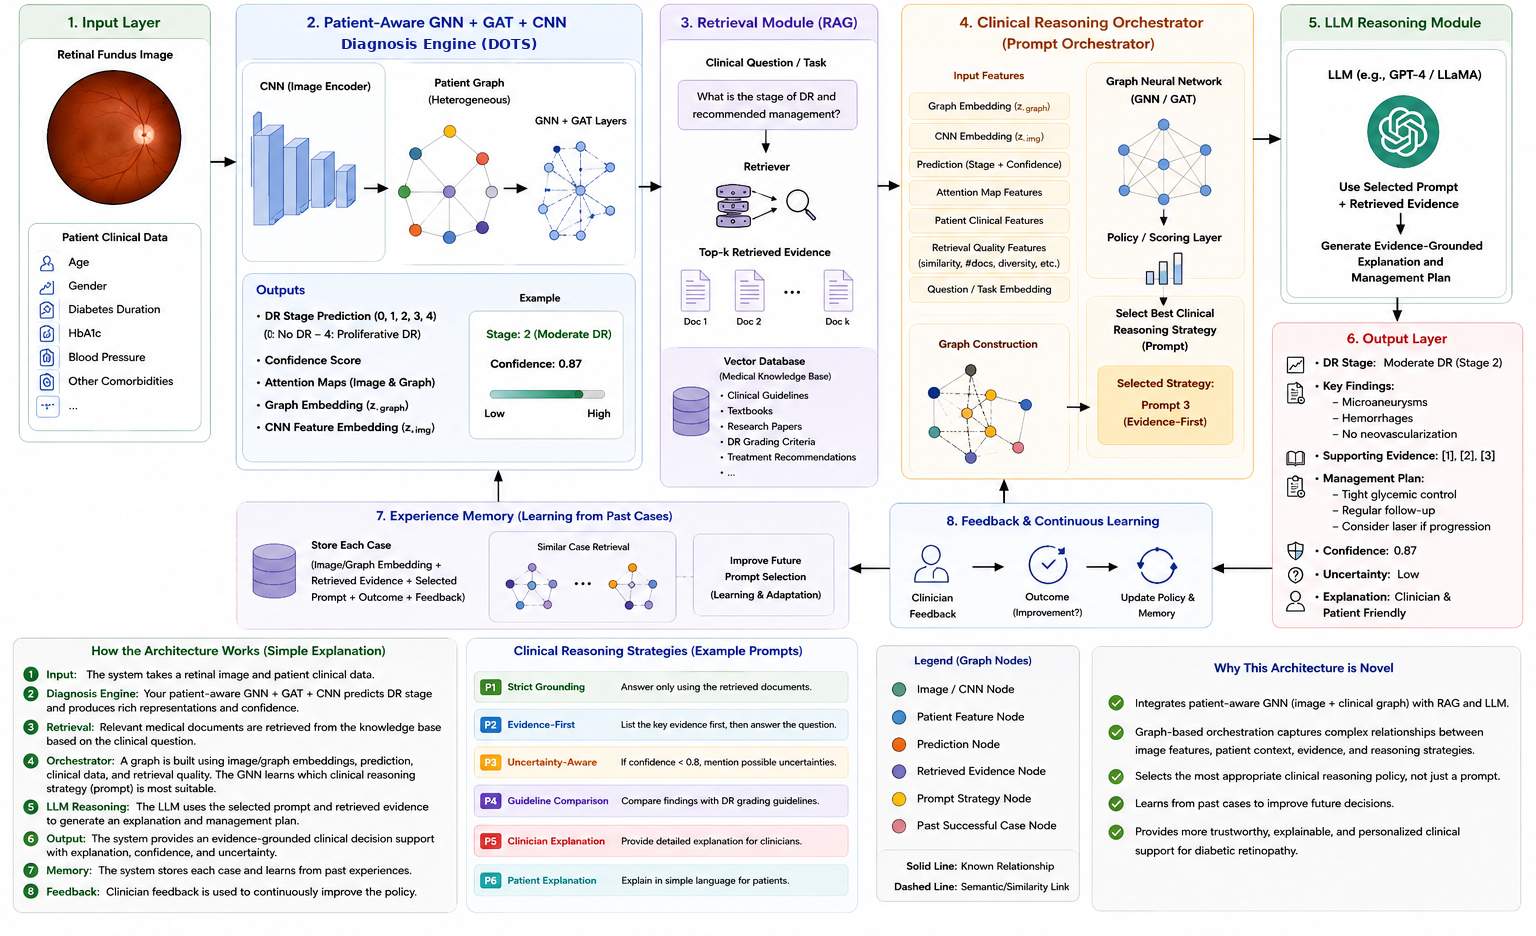
\includegraphics[width=\linewidth,height=0.9\textheight,keepaspectratio]{fig_llm_orchestration}
\caption[Patient-aware graph-driven prompt orchestration (future work)]{Patient-aware
graph-driven prompt orchestration for explainable, retrieval-augmented clinical decision
support in diabetic retinopathy (future work, not implemented). The eight modules are
described in \cref{sec:llm}.}
\label{fig:llm}
\end{figure}
\end{landscape}}


Such an extension raises questions outside the scope of this thesis, chiefly how to
prevent a fluent narrative from overriding or contradicting the CORAL ranking and the
abstention decision, which are the load-bearing safety mechanisms. An unfaithful
narrative would undermine exactly the transparency this chapter was designed to provide.
No LLM experiments were conducted; this subsection is a scoped direction for future work.

Should such a layer be built, it would need its own evaluation criteria, distinct from
those of the grading model: \emph{faithfulness} (every statement in the narrative must be
traceable to a logged quantity), \emph{consistency} (the narrative must never contradict the
grade, the confidence or the abstention decision), and \emph{usefulness}, measured with
clinicians and patients in the reader study of Phase~2. These criteria could be
pre-specified in the same way as H1--H3.

\section{Ethical Considerations}
\label{sec:ethics}

Three ethical considerations go beyond formal regulatory requirements.

\paragraph{Algorithmic fairness across demographic subgroups.}
The five benchmarks (\cref{app:datasets}) come from the United States, India, France and
China, which gives some geographic and probably some ethnic diversity. None of them,
however, provides per-image demographic metadata (age, sex, ethnicity), which prevents a
formal subgroup fairness analysis. This is stated as a limitation (\cref{sec:limits-gc})
rather than elided.

\paragraph{Deskilling risk.}
Reliance on automated screening may, over time, erode human grading skill. By routing
$6.2\%$ of cases -- the most challenging ones -- to human review, entropy abstention keeps
graders actively practising on difficult cases rather than removing them from the
workflow.

\paragraph{Accountability for missed referrals.}
Even at Sev-NR $=1.9\%$, some severe cases will be missed. The audit trail of
\cref{sec:audit} makes every missed case traceable to a logged prediction with its full
explanation, which supports clinical-governance review. It does not settle the broader
question of legal and professional accountability when an automated system contributes
to a missed diagnosis; that question is left to the regulatory and legal review of
Phases~3--4 (\cref{sec:roadmap}). In all cases, DOTS is designed as a decision-support tool: the responsibility for the final referral decision remains with the clinician.

\section{What Regulatory-by-Construction Does Not Solve}
\label{sec:regnotsolve}

Designing for compliance from the outset avoids a specific class of late architectural
surgery; it is worth being equally explicit about what it does not solve. Mapping DOTS to
IEC~62304, ISO~14971 and the EU AI Act (\cref{tab:regmap}) documents
\emph{architectural} compliance: the system has the structural features (typed
interfaces, FMEA, audit logging, abstention) that a notified body would expect. It does
not constitute the conformity assessment, clinical evaluation or notified-body review
required before CE marking; those remain Phase~2--4 activities outside the scope of a
doctoral thesis. Likewise, the FHIR gap of \cref{sec:fhir} is not a hypothetical risk: it
is the concrete reason why DOTS could not be connected to a live clinical workflow today.

The honest claim is therefore narrower than ``DOTS is compliant'': DOTS's architecture was
shaped by the requirements it will eventually need to satisfy. This has a practical
consequence for replication. Because each compliance property is embedded in the pipeline
rather than asserted afterwards, any laboratory that reproduces the six-stage pipeline
with the released code (\cref{app:repro}) also reproduces these properties; the FHIR
adapter is the only element that requires site-specific work before clinical use. The
results of \cref{ch:toporet,ch:dots} constitute Level~1 (computational) evidence
in the roadmap of the General Conclusion; regulatory clearance (Level~4) requires
prospective validation, notified-body assessment and post-market surveillance, none of
which is conducted here.

\section{Towards Clinical Deployment: Translation Roadmap}
\label{sec:roadmap}\label{app:roadmap}

The regulatory-oriented design of this chapter prepares DOTS for certification, but does
not replace the clinical evidence that certification requires. The translation of DOTS
into clinical practice is therefore planned in four phases (\cref{tab:roadmap}), following
the four levels of evidence used in diagnostic AI evaluation: Level~1 computational
evidence, Level~2 prospective agreement with human readers, Level~3 randomised patient
outcomes, and Level~4 regulatory clearance. This thesis provides Level~1 evidence only.

\begin{table}[!tb]
\centering
\caption[Four-phase clinical translation roadmap]{Four-phase clinical translation roadmap.}
\label{tab:roadmap}
\small
\begin{tabular}{@{}c l P{7.6cm} l l@{}}
\toprule
Phase & Period & Key deliverable & Evidence & Status \\
\midrule
1 & 2023--2026 & Nine publications; five-benchmark validation; necessity proof & Level 1 & Complete \\
2 & 2026--2027 & Multi-site reader study ($\geq3$ sites, $N\geq200$, pre-registered); FHIR R4 adapter & Level 2 & Planned \\
3 & 2027--2028 & Randomised trial: AI-assisted versus standard-of-care screening & Level 3 & Planned \\
4 & 2028--2029 & CE marking (EU AI Act, high-risk); FDA 510(k) or De Novo & Level 4 & Planned \\
\bottomrule
\end{tabular}
\end{table}

Phase~2 is the critical next step. It combines a pre-registered, multi-site reader study
($N\geq200$ patients, at least three sites), in which board-certified ophthalmologists
grade images with and without DOTS, with the implementation of the FHIR~R4 adapter of
\cref{sec:fhir}. Its primary success criterion is a Sev-NR below $2\%$ with the upper
bound of its 95\% confidence interval also below $2\%$, which would close the main
statistical limitation of the present results. Ethics approval and the FHIR adapter have no
technical dependency and can proceed in parallel. The dates of Phases~2--4 are indicative:
they depend on clinical and industrial partnerships beyond the doctoral work.

\section*{Conclusion}
\phantomsection\addcontentsline{toc}{section}{Conclusion}

This chapter mapped DOTS to IEC~62304, ISO~14971 and the EU AI Act by construction
(\cref{tab:regmap}), documented a 47-test verification suite with full interface coverage
of the six stages, and identified the FHIR R4 adapter (Tier~3) as the main remaining
barrier between a computationally validated system and a clinically deployed product.
Per-patient inference ($31.4$~ms) does not depend on cohort size, so the inductive design
choice of \cref{ch:found} carries through to deployment scale. The three-tier
architecture decouples the validated inference engine from site-specific integration.
Three ethical considerations -- fairness, deskilling and accountability -- are identified
for explicit future work. The General Conclusion now brings together the contributions of the thesis, their
practical value, their limits and the perspectives they open.


\chapter*{General Conclusion}
\addcontentsline{toc}{chapter}{General Conclusion}
\markboth{General Conclusion}{}
\label{ch:conclusion}

This thesis addressed the automated grading of diabetic retinopathy in a context where
screening needs grow much faster than the number of human graders, and where an automated
system is only acceptable if it is both accurate and safe for patients. Starting from a
review of a decade of deep-learning methods, we showed that every published system shares
three architectural limitations: it grades each image in isolation, it ignores the global
topology of the vascular network, and it must answer even when the image is ambiguous.
The whole work was organised around resolving these three limitations together.

The study began with the clinical context of the disease and the methodological tools
needed to address the three limitations: graph neural networks, persistent homology,
ordinal regression and calibrated abstention. We then validated the graph template outside
medicine, on microservice and network-security graphs, and gathered the first evidence,
with three independent methods, that structural and topological features of the retina
carry information that deep visual features miss. These results led to TOPORET, an
inductive population graph whose edges combine visual and topological similarity. Its
pre-specified tests confirmed that the graph brings a significant gain over independent
classification ($t_4=3.82$, $p=0.009$) and that topological features are strongly
associated with severity ($F(4,4995)=1308.9$, $\eta^2=0.51$). TOPORET, however, remained
above the safety threshold. The final system, DOTS, added a retinal foundation model, an
ordinal head with guaranteed rank consistency and entropy-based abstention. On five public
benchmarks it meets the seven predefined criteria at the point estimate (QWK $=0.951$,
Sev-NR $=1.9\%$, $0\%$ rank violations), and an exhaustive enumeration showed that none of
its six reduced versions does. Finally, the system was engineered as medical-device
software whose design maps onto the IEC~62304 and ISO~14971 standards and the EU AI Act.

The three research questions of the thesis can therefore be answered as follows. Does
the relational context between patients carry information that a per-image classifier
cannot recover? Yes, provided that the graph is built with a similarity that includes the
topology of the vessels; a visual similarity alone is not enough. Is the global topology
of the vascular network related to the severity of the disease? Yes, strongly, with the
largest effects for the loops that appear with neovascularisation. Can a single
architecture meet all the predefined criteria of accuracy, calibration and safety, and are
all of its components needed? Yes at the point estimate, and none of its reduced versions
does, although the confidence interval of the safety criterion still calls for prospective
confirmation.

The contributions of this research are both scientific and practical. On the scientific
side, the thesis shows that the three limitations of automated DR grading can be resolved
in a single architecture, and that the three components are complementary rather than
interchangeable: within the evaluated family, removing any of them loses the safety
criterion. It also introduces the use of persistent-homology descriptors of the vessel
skeleton inside the similarity of a population graph, and a validation discipline in which
every hypothesis, test and threshold is fixed before the experiment. On the practical side,
DOTS grades an image in $31.4$~ms on a single GPU, defers only $6.2\%$ of images to human
graders, explains each decision with the similar cases and topological features that
support it, and is designed to be verified and certified. Under explicit prevalence
assumptions, it would avoid about $600$ missed sight-threatening cases per year in a
programme of $500{,}000$ patients. A CPU model developed along the way (SAMF-GB) also
offers a low-cost alternative for settings without GPUs.

Beyond its results, the research programme taught several methodological lessons that may
be useful to other work on medical AI. First, accuracy and safety must be measured
separately: every system in this thesis gained QWK long before it crossed the safety
threshold, and optimising the former does not guarantee the latter. Second, validating an
architectural idea outside medicine, where data are plentiful and labels unambiguous, made
the medical experiments easier to design and to interpret. Third, fixing hypotheses, tests
and thresholds before running the experiments turned some results that could have been
discarded, such as the non-significant visual-only graph, into informative findings.
Fourth, designing for regulation from the start cost little and avoided late changes to the
architecture. Finally, the most useful component for safety was not the most accurate one:
entropy-based abstention adds less than one point of QWK, but it is the step that brings
the non-referral rate below the threshold.

\phantomsection\label{sec:limits-gc}

These results must be read within clear limits. All experiments are retrospective, on
curated public datasets; the upper bound of the 95\% confidence interval of Sev-NR
($2.4\%$) is still above the $2\%$ threshold, so statistical compliance with the safety
criterion is not yet established. Performance is lower on the smallest dataset (IDRiD,
$516$ images), where the population graph is sparse. None of the datasets provides
demographic information, so fairness across age, sex and ethnicity could not be assessed.
The population graph uses a single visit per patient and ignores the progression of the
disease over time. Finally, the computation of topological features is the main latency
bottleneck, and the integration with hospital information systems (FHIR adapter) is
designed but not yet implemented.

These limits open several directions for future work. The most immediate is a
prospective, multi-site reader study, pre-registered, to confirm the safety of DOTS in
real screening conditions and to reduce the uncertainty on Sev-NR; it is the first step of
the four-phase translation roadmap of \cref{sec:roadmap}, which leads to a randomised
trial and to CE marking and FDA submission. On the methodological side, learnable
topological layers could replace the hand-crafted persistence vector and possibly improve
accuracy, provided that they remain interpretable. A temporal population graph, linking the
successive visits of each patient, could exploit the speed of progression at the difficult
Grade~2/3 boundary. Federated construction of the population graph would allow several
hospitals to collaborate without sharing patient data. Smartphone-based fundus capture,
connected to the DOTS inference service, could extend screening to low-resource settings.
Finally, an explanation layer based on large language models could turn the logged evidence
into narratives adapted to clinicians and patients, under strict safeguards that prevent
it from contradicting the grade or the decision to abstain.

More broadly, the three-axis framework -- relational graph, structural topology, and
ordinal prediction with safe abstention -- is not specific to the retina. It can serve as a
template for any graded disease with an ordinal severity scale, a structural anatomical
prior and a safety threshold, such as age-related macular degeneration or glaucoma.

In summary, this work contributes to making automated screening of diabetic retinopathy
not only more accurate, but also safer, more transparent and closer to clinical use. The
code, models and configurations are released for independent reproduction, and the
remaining steps towards deployment are clearly identified. The prevention of blindness at
the scale of a population will depend on the ability to carry such systems from
computational validation to everyday clinical practice.


% ------------------------------------------------------------ back matter
\cleardoublepage
\phantomsection
\addcontentsline{toc}{chapter}{Bibliography}
\markboth{Bibliography}{}
\bibliographystyle{unsrt}
\bibliography{references}

\chapter*{List of Publications}
\addcontentsline{toc}{chapter}{List of Publications}
\markboth{List of Publications}{}
\label{ch:pubs}

The thesis is supported by twelve publications: six conference papers (three published,
three accepted and to appear), two book chapters accepted and to appear, and four journal
articles under review or revision.

\section*{Conference Papers}

\begin{description}[style=sameline,leftmargin=3.2em,labelwidth=2.6em,itemsep=4pt]
\item[{[P1]}] N.~Belhadj, M.~A.~Mezghich, J.~Fattahi, L.~Latrach. ``GNN-MSOrchest: Graph
Neural Networks Based Approach for Micro-Services Orchestration -- A Simulation Based Design
Use Case.'' \emph{17th ICAART}, vol.~3, pp.~933--939, SCITEPRESS, 2025.
doi:10.5220/0013238200003890.
\item[{[P2]}] N.~Belhadj, M.~A.~Mezghich, L.~Latrach, R.~Ghayoula. ``Leveraging Local
Invariants and Graph Neural Networks for Enhanced Anomaly Detection in Distributed
Systems.'' \emph{18th ICAART}, vol.~2, pp.~1090--1101, SCITEPRESS, 2026.
\item[{[P3]}] N.~Belhadj, M.~A.~Mezghich, J.~Fattahi, R.~Ghayoula, L.~Latrach. ``Hybrid
CNN-GNN Model for Retinopathy Classification Using Geometric and Topological Invariants.''
\emph{18th ICAART}, vol.~5, pp.~4635--4642, SCITEPRESS, 2026.
\item[{[P4]}] N.~Belhadj, M.~A.~Mezghich, J.~Fattahi, R.~Ghayoula, L.~Latrach. ``A
High-Precision Hybrid Intelligence Framework for Diabetic Retinopathy Grading.''
\emph{International Conference on Pattern Recognition Applications and Methods (ICPRAM)},
SCITEPRESS, 2026. Short paper; to appear.
\item[{[P5]}] N.~Belhadj, M.~A.~Mezghich, R.~Ghayoula, L.~Latrach. ``A Graph-Based
Software Framework with Topological Analysis of Retinal Vessel Networks for Automated
Diabetic Retinopathy Grading.'' \emph{International Conference on Evaluation of Novel
Approaches to Software Engineering (ENASE)}, 2026. Best Paper candidate; to appear.
\item[{[P6]}] N.~Belhadj, R.~Ghayoula, L.~Latrach. ``Cross-Dataset Generalisation of
Topological Features for Retinal Image Grading.'' \emph{Medical Image Understanding and
Analysis (MIUA)}, 2026. Oral presentation; to appear.
\end{description}

\section*{Book Chapters (Accepted, to Appear)}

\begin{description}[style=sameline,leftmargin=3.2em,labelwidth=2.6em,itemsep=4pt]
\item[{[B1]}] N.~Belhadj, M.~A.~Mezghich, L.~Latrach, R.~Ghayoula. ``Adaptive
Invariant-Augmented Graph Feature Propagation for Anomaly Detection in Networked Systems.''
In \emph{Agents and Artificial Intelligence}, Lecture Notes in Artificial Intelligence,
Springer, 2026. Extended version of [P2].
\item[{[B2]}] M.~A.~Mezghich, N.~Belhadj, L.~Latrach, J.~Fattahi, R.~Ghayoula.
``Topology-Aware Hybrid CNN--GNN Framework for Robust Diabetic Retinopathy Screening.'' In
\emph{Agents and Artificial Intelligence}, Lecture Notes in Artificial Intelligence,
Springer, 2026. Extended version of [P3].
\end{description}

\section*{Journal Articles (Under Review or Revision)}

\begin{description}[style=sameline,leftmargin=3.2em,labelwidth=2.6em,itemsep=4pt]
\item[{[J1]}] N.~Belhadj, L.~Latrach, R.~Ghayoula, M.~A.~Mezghich. ``DOTS:
Ordinal-Supervised Multi-Source Diabetic Retinopathy Grading with Feature Refinement
Encoder and CORAL Regression.'' \emph{SN Computer Science}, under review.
\item[{[J2]}] N.~Belhadj, M.~A.~Mezghich, L.~Latrach. ``SAMF-GB: Structural Anatomical
Multi-Family Features with Gradient Boosting for Ordinal Diabetic Retinopathy Grading.''
\emph{SN Computer Science}, under review.
\item[{[J3]}] N.~Belhadj, M.~A.~Mezghich, J.~Fattahi, R.~Ghayoula, L.~Latrach. ``A
Graph-Based Deep Learning Framework for Diabetic Retinopathy Classification with
Topology-Aware Feature Augmentation.'' \emph{PLOS ONE}, under revision.
\item[{[J4]}] N.~Belhadj, M.~A.~Mezghich, L.~Latrach, R.~Ghayoula. ``Topology-Regularised
Population Graph Learning for Diabetic Retinopathy Grading via Multi-Source Data
Fusion.'' \emph{Machine Vision and Applications}, under review.
\end{description}

\section*{Author Contributions (CRediT)}

\textbf{Nader Belhadj:} conceptualisation, methodology, software, validation, formal
analysis, investigation, data curation, writing (original draft), visualisation.
\textbf{Lassaad Latrach:} supervision, methodology (statistical pre-specification and
falsification criteria), writing (review and editing), project administration.
\textbf{Ridha Ghayoula:} co-supervision, methodology (topological data analysis),
resources (Laval University research exchange), writing (review and editing).
\textbf{Mohamed Amine Mezghich:} co-advising, software architecture and
regulatory-oriented design, writing (review and editing).
All authors approved each publication on which they appear.


\appendix
\inappendixtrue
\renewcommand{\thefigure}{\thechapter.\arabic{figure}}
\renewcommand{\thetable}{\thechapter.\arabic{table}}
% ===========================================================================
\chapter{Consolidated Numerical Results}
\label{app:results}
\lotgroup{Appendix A -- Consolidated Numerical Results}

\Cref{tab:experiments} lists the twelve principal experiments in chronological order.

\begin{table}[H]
\centering
\caption[The twelve principal experiments, in chronological order]{The twelve principal experiments, in chronological order.}
\label{tab:experiments}
\small
\begin{tabular}{@{}c P{4.6cm} l P{4.3cm} r@{}}
\toprule
\# & Experiment & Publication & Primary result & $N$ \\
\midrule
1 & GraphSAGE microservice orchestration & P1~\cite{belhadj2025icaart} & Cascade containment $81\%$ & 48 nodes \\
2 & Invariant-augmented GNN anomaly detection & P2, B1~\cite{belhadj2026invariants,belhadj2026lnaiinv} & F1 $94.4$--$97.0\%$ (P2); no significant F1 gain from invariants over ten runs (B1) & 4 datasets \\
3 & Hybrid CNN--GNN $+$ geometric and topological invariants & P3, B2~\cite{belhadj2026hybrid,mezghich2026lnaitopo} & $95.1\%$ binary accuracy ($+7.0$~pp) & 3{,}662 \\
4 & LightGBM-HC (hand-crafted, Messidor-2) & P4~\cite{belhadj2026icpram} & QWK $=0.858$, $1.6$~ms CPU classifier & 1{,}748 \\
5 & SAMF-GB & J2~\cite{belhadj2026samfgb} & QWK $=0.882$, $2.1$~ms CPU & 88{,}702 \\
6 & TOPORET on Kaggle DR & J3~\cite{belhadj2025plos} & QWK $=0.88$, accuracy $95.5\%$ & 88{,}702 \\
7 & TOPORET on Messidor-2 and APTOS 2019 & J3~\cite{belhadj2025plos} & QWK $=0.90$ and $0.86$ & 1{,}748; 3{,}662 \\
8 & H1 graph-contribution test & J3~\cite{belhadj2025plos} & $t_4=3.82$, $p=0.019$, $d_z=1.71$ & 88{,}702 \\
9 & H2 topological ANOVA & J3~\cite{belhadj2025plos} & $F=84.3$, $p<0.001$ & Kaggle DR \\
10 & DOTS in distribution & J1~\cite{belhadj2026dots} & QWK $=0.951$ & 88{,}702 \\
11 & DOTS H3a seven-criterion evaluation & J1~\cite{belhadj2026dots} & $7/7$ criteria met at the point estimate & 10{,}000 \\
12 & H3b necessity enumeration (investigated family) & J1~\cite{belhadj2026dots} & $6/6$ proper subsets fail & 10{,}000 \\
\bottomrule
\end{tabular}
\tabnote{$N$ is a number of images (or of graph nodes for experiments 1--2), not
necessarily of independent patients.}
\end{table}

\paragraph{Reading the sequence.}
The experiments are ordered chronologically rather than thematically, and the progression
is informative in itself. Experiments 1--2 evaluate the graph template entirely outside
medicine; the ten-run re-evaluation of experiment~2 revised its accuracy claim, leaving
interpretability as the main benefit of the invariants. Experiments 3--5 move to diabetic retinopathy at the proof-of-concept level,
each isolating one candidate signal against a fixed baseline. Experiments 6--9 form the
TOPORET evaluation, ending with the two confirmatory tests (8--9) that decide H1 and H2.
Experiments 10--12 apply the same discipline to DOTS and H3; experiment 12 is the most
computationally demanding of the programme, with six independently trained subset
architectures evaluated against all seven criteria under one protocol. The necessity enumeration (12) uses the $10{,}000$-image test set of the H3a evaluation, so
that DOTS and every proper subset are compared on identical data.


% ===========================================================================
\chapter{Hyperparameter Reference}
\label{app:hyper}
\lotgroup{Appendix B -- Hyperparameter Reference}

\Cref{tab:hyper} lists every hyperparameter of TOPORET and DOTS side by side.

\begin{table}[H]
\centering
\caption[Hyperparameter reference]{Hyperparameter reference: TOPORET versus DOTS.}
\label{tab:hyper}
\small
\begin{tabular}{@{}P{4.4cm}P{5.0cm}P{4.6cm}@{}}
\toprule
Hyperparameter & TOPORET~\cite{belhadj2025plos} & DOTS \\
\midrule
Backbone & EfficientNet-B3 (frozen) & RETFound ViT-L/16 (frozen) \\
Topological vector & 6-D (\cref{eq:tda-toporet}) & 7-D (\cref{eq:tda}) \\
Output head & Softmax, class-weighted CE & CORAL (architectural) \\
Graph construction & Threshold $\tau=0.65$, exact pairs & $k$-NN, $k=15$ (FAISS) \\
$\alpha$ (visual/topological balance) & 0.6 & 0.65 \\
Graph layer & GraphSAGE (mean) & Dynamic GAT \\
$d_h$ (hidden dimension) & 256 & 256 \\
$L$ (GNN layers) & 2 & 2 \\
$S$ (samples per layer) & 10 & 25 \\
Dropout $p$ & 0.30 & 0.30 \\
Class weights & $w_c=N/(C\,N_c)$ & $1.0, 2.5, 3.0, 8.0, 6.0$ \\
Label smoothing $\epsilon$ & -- & 0.05 \\
Abstention threshold $\tau_U$ & -- & 0.73~nats \\
Severe-DR referral threshold $t$ & -- & \refT{} (validation; frozen before test) \\
Referral rule & Not applicable & Refer if $\hat P(Y\geq3)>t$ or $H_i>\tau_U$ (\cref{eq:referral}) \\
Optimiser & Adam, lr $10^{-3}\to10^{-5}$ (cosine) & Adam, lr $=10^{-3}$ \\
Batch size & 64 & 32 \\
Epochs & $\leq200$, early stopping (20) & 100 \\
Data splits & 5 patient-aware $70/10/20$ & 5 folds, stratified \\
\bottomrule
\end{tabular}
\tabnote{The ordinal variant of TOPORET used as the starting point of DOTS
(\cref{ch:dots}) keeps the TOPORET architecture (dual-similarity GraphSAGE and topological
features) with a CORN head, and is trained under the DOTS protocol and graph settings.}
\end{table}

\paragraph{Reading the comparison.}
TOPORET and DOTS were developed under different protocols, and their hyperparameters
differ beyond the components that address Gaps~A--C (\cref{sec:ch4-gaps}): the
topological vector, the graph construction ($\tau$-threshold with exact pairwise
distances versus FAISS $k$-NN), the sampling depth, the optimisation schedule and the data
splits. The TOPORET-to-DOTS ablation of \cref{tab:ablate} is therefore performed within
the DOTS protocol, starting from the ordinal variant of TOPORET, so that each gap
resolution is introduced as an isolated change. The TOPORET hyperparameters were selected
on validation data (\cref{tab:hparam}).

% ===========================================================================
\chapter{Statistical Test Reference}
\label{app:stats}
\lotgroup{Appendix C -- Statistical Test Reference}

This appendix collects the formal statement of every statistical test used in the thesis.
Each hypothesis was pre-specified: before any experimental result was seen, the null
hypothesis, the test statistic, the significance threshold and the effect-size metric were
fixed. \Cref{tab:falsif} lists, for each claim, the outcome that would have falsified it,
the observed result and the margin by which the claim survived.

\begin{table}[H]
\centering
\caption[Falsification criteria and observed margins]{Falsification criteria and observed margins.}
\label{tab:falsif}
\small
\begin{tabular}{@{}P{4.2cm}P{3.0cm}P{4.3cm}P{2.9cm}@{}}
\toprule
Claim & Falsified if & Observed & Margin \\
\midrule
H1 -- graph QWK gain & $|t_4| < 2.78$ & $t_4=3.82$, $p=0.019$ & $\times1.37$ critical \\
H2 -- topology linked to severity & $F < 3.72$ & $F=84.3$, $p<0.001$ & $\times23$ critical \\
H3a -- all seven criteria & any criterion violated & $7/7$ met at the point estimate (\cref{tab:h3a}) & Sev-NR CI $[1.4\%,2.4\%]$ crosses $2\%$ \\
H3b -- necessity (investigated family) & any proper subset has Sev-NR $<2\%$ & $6/6$ proper subsets fail & constructive, scoped \\
CORAL violations & any violation at test time & $0.0\%$ & algebraic identity \\
Sev-NR point estimate & $\geq 2.0\%$ & $1.9\%$ $[1.4\%,\,2.4\%]$ & $0.1$~pp \\
\bottomrule
\end{tabular}
\tabnote{The critical values are $t_{0.025,4}=2.78$ (the conservative threshold adopted
for H1) and $F_{0.005;\,4,\,\infty}\approx3.72$ (conservative level used for H2); see
\cref{app:stats}.}
\end{table}

\paragraph{Notation convention.}
\textbf{H1}, \textbf{H2}, \textbf{H3} (upright) denote the three research hypotheses.
$H_0$ and $H_1$ (italic, subscript, in math mode) denote the zeroth and first
persistent-homology groups. The two notations are unrelated: hypothesis H2 is tested
using $H_0$ and $H_1$ features as independent variables.


\section{H1: Paired \texorpdfstring{$t$}{t}-Test}
\begin{align}
H_0 &: \mu_{\Delta\mathrm{QWK}} = 0 \quad \text{(the graph gives no QWK change)}, \\
H_a &: \mu_{\Delta\mathrm{QWK}} \neq 0 \quad \text{(the graph changes the QWK)}, \\
t &= \frac{\bar d}{s_d/\sqrt{n}}, \qquad \mathrm{df}=n-1=4,
\end{align}
where $\bar d$ is the mean of the five per-split QWK differences (TOPORET minus the CNN
baseline, over five patient-aware $70/10/20$ splits) and $s_d$ their standard deviation. Because the inferential unit is the
data split, the test has four degrees of freedom; the bootstrap and exact
permutation analyses of \cref{sec:testimpl} are complementary robustness checks on the
same five differences, not independent replications. The test is two-tailed, with
critical value $t_{0.025,4}=2.776$ at $\alpha=0.05$. Observed: $t_4=3.82$, two-tailed
$p=0.019$ (one-tailed $0.009$), on Kaggle DR; $t_4=4.1$ ($p=0.015$) on Messidor-2 and
$t_4=3.5$ ($p=0.025$) on APTOS~2019~\cite{belhadj2025plos}.

\section{H2: One-Way ANOVA}
\begin{align}
H_0 &: \mu_{G_0}=\mu_{G_1}=\cdots=\mu_{G_4} \quad \text{for total $H_1$ persistence } \Pi_{H_1}, \\
H_a &: \text{at least one } \mu_{G_k} \text{ differs}, \\
F &= \frac{\mathrm{MS}_{\mathrm{between}}}{\mathrm{MS}_{\mathrm{within}}}, \qquad
\mathrm{df}_1=4 .
\end{align}
A single primary feature, $\Pi_{H_1}$, is tested, at the conservative level $\alpha=0.005$;
for the large samples of Kaggle DR the critical value is $F_{0.005;\,4,\,\infty}\approx3.72$.
Post-hoc: Tukey HSD~\cite{tukey1949} on the pairwise grade comparisons. Observed:
$F=84.3$, $p<0.001$~\cite{belhadj2025plos}.

\section{H3a: Bootstrap Confidence Intervals}
For each of the seven criteria of \cref{tab:h3a}, a 95\% confidence interval is computed
by stratified bootstrap~\cite{efron1993bootstrap} ($B=10{,}000$ resamples, stratified by
true grade to preserve the class distribution). A criterion ``passes'' if its point
estimate meets the threshold; the interval is reported for transparency, but the
pre-specified decision rule uses the point estimate, except where explicitly stated (the
Phase~2 success criterion requires the interval).

\section{H3b: Constructive Enumeration}
No inferential test applies to H3b. The claim is established by constructing and
evaluating all six proper subsets against the same seven-criterion specification
(\cref{sec:h3b}). Claims of the form ``no member of this finite, fully enumerable set
satisfies property $P$'' are best established by exhaustive verification, since the whole
set is evaluated. The set, however, is the six subsets \emph{as implemented} in the
investigated family; the result does not extend to every conceivable architecture lacking
one of the axes, and each subset's Sev-NR is itself an estimate with sampling uncertainty. The price of this rigour is computational: every proper subset must be trained and evaluated on all benchmarks (\cref{tab:compute}).

\section{Effect-Size Formulae}
\begin{align}
d &= \frac{\bar x_1-\bar x_2}{s_{\mathrm{pooled}}}, \qquad
s_{\mathrm{pooled}} = \sqrt{\frac{(n_1-1)s_1^2+(n_2-1)s_2^2}{n_1+n_2-2}}, \\
d_z &= \frac{\bar\delta}{s_\delta} = \frac{t}{\sqrt{n}}, \\
\eta^2 &= \frac{\mathrm{SS}_{\mathrm{between}}}{\mathrm{SS}_{\mathrm{total}}}
        = \frac{df_1\,F}{df_1\,F+df_2} .
\end{align}
The first formula is used for comparisons between independent groups; the second, where
$\bar\delta$ and $s_\delta$ are the mean and standard deviation of the paired differences
over the $n$ splits, is used for the paired $t$-test of H1 ($d_z=3.82/\sqrt5=1.71$); the third
relates $\eta^2$ to the $F$ statistic of a one-way ANOVA, and requires the within-groups
degrees of freedom $df_2$, which are not reported with the H2 statistic
in~\cite{belhadj2025plos}.
Effect sizes complement $p$-values: a $p$-value says whether an effect is likely to be
real, an effect size says how large it is, independently of the sample size. With the large
samples used in this thesis, even negligible differences can reach significance, which is
why every primary comparison is reported with its effect size. \Cref{tab:effthresh} gives
the conventional interpretation thresholds~\cite{cohen1988}; all standardised effect sizes
reported in \cref{tab:effects} meet or exceed the ``large'' threshold.

\begin{table}[H]
\centering
\caption{Conventional thresholds for the interpretation of effect sizes.}
\label{tab:effthresh}
\small
\begin{tabular}{@{}lccc@{}}
\toprule
Measure & Small & Medium & Large \\
\midrule
Cohen's $d$ (difference of two means) & 0.2 & 0.5 & 0.8 \\
$\eta^2$ (share of variance explained, ANOVA) & 0.01 & 0.06 & 0.14 \\
\bottomrule
\end{tabular}
\end{table}

\section{Control of Multiple Comparisons}

Testing many hypotheses on the same data increases the chance of a false positive. Three
measures limit this risk in the thesis. First, each research hypothesis has a single
pre-specified primary test and a single primary metric, fixed before the experiment
(\cref{tab:falsif}); secondary analyses, such as the bootstrap and permutation tests of H1,
are reported as supporting evidence and do not change the decision. Second, when several
tests address the same hypothesis, as for the topological features of H2, the significance
level is corrected with the Bonferroni method and lowered further for conservatism. Third,
the necessity claim H3b does not rely on a statistical test at all, since the six proper
subsets form the complete set of alternatives within the investigated family and are all
evaluated.

% ===========================================================================
\chapter{Reproducibility and Software Environment}
\label{app:repro}
\lotgroup{Appendix D -- Reproducibility and Software Environment}

\section{Code and Data Availability}
All code, model weights and configuration files described in this thesis are released
under the Apache~2.0 licence at \url{https://github.com/Nader-BelHadj/plosene} upon
acceptance of the DOTS article~\cite{belhadj2026dots}. The release includes the source
code of the six pipeline stages (\cref{tab:stages}), the 47-test verification suite
(\cref{tab:unittests}), YAML configurations for the twelve principal experiments
(\cref{app:results}), a Dockerfile that pins every software dependency, and the
evaluation manifest \texttt{test\_manifest.csv} listing the identifier, source dataset and
grade of each image of the H3a test set (\cref{tab:testcomp}). The five
datasets are public and must be obtained from their original distributors
(\cref{app:datasets}).

\section{Software Environment}
\Cref{tab:software} lists the software components and their versions.
\begin{table}[H]
\centering
\caption[Software environment and key library versions]{Software environment and key library versions.}
\label{tab:software}
\small
\begin{tabular}{@{}l P{10.4cm}@{}}
\toprule
Component & Version / use \\
\midrule
Python & 3.10 \\
PyTorch~\cite{paszke2019pytorch} & 2.1, CUDA 12.1 \\
PyTorch Geometric~\cite{fey2019pyg} & 2.4 (GraphSAGE and GAT implementations) \\
GUDHI~\cite{maria2014gudhi} & 3.9 (Vietoris--Rips persistent homology, stage S3) \\
FAISS~\cite{johnson2021faiss} & 1.7 (approximate $k$-NN, stage S5) \\
timm & Version pinned in the Dockerfile (RETFound and EfficientNet-B3 loading) \\
scikit-learn~\cite{pedregosa2011sklearn} & 1.3 (evaluation metrics) \\
SciPy & ANOVA and $t$-tests (\cref{sec:testimpl}) \\
OpenCV & 4.8 (CLAHE and Zhang--Suen skeletonisation, stage S1) \\
\bottomrule
\end{tabular}
\end{table}

\Cref{tab:hardware} lists the hardware used at each stage of the programme. All timings reported in the thesis were measured on this hardware, so that latency and cost figures can be compared directly across chapters.

\begin{table}[!tb]
\centering
\caption[Hardware used for training, benchmarking and testing]{Hardware used for training, benchmarking and testing.}
\label{tab:hardware}
\small
\begin{tabular}{@{}l P{9.6cm}@{}}
\toprule
Context & Hardware \\
\midrule
Model training (all experiments) & $1\times$ NVIDIA A100 (40~GB), 16-core CPU, 128~GB RAM \\
Inference latency (\cref{tab:latency}) & $1\times$ NVIDIA A100 (stages S2, S5, S6); 16-core CPU (stage S3) \\
Unit-test suite & CPU only, any modern x86-64 workstation \\
\bottomrule
\end{tabular}
\end{table}

\section{Randomness and Seeding}
The primary experiments use a single global seed (42) for all stochastic operations: model
initialisation, data-loader shuffling, cross-validation fold assignment and bootstrap
resampling. The stability analysis of \cref{sec:numrepro} repeats the main experiments with two
additional seeds (123 and 7).
Five-fold splits are stratified by ICDR grade, computed once per experiment and held fixed
across all ablation variants (\cref{tab:ablate,tab:ablation3}), so that differences
between configurations are not confounded by different splits. The unit of every split and
of every reported sample size is the retinal image. Some benchmarks contain several images
of the same patient (for example both eyes in Kaggle EyePACS), so the reported results are
image-level estimates and patient-level generalisation is interpreted cautiously.

\section{Reproducibility Tolerance}
\label{sec:tolerance}
Because some GPU kernels are not bit-exact across hardware generations even with fixed
seeds, results within $2\sigma$ of the reported values -- with $\sigma$ the five-fold
standard deviation reported with each primary metric (for example \cref{tab:h1}) -- are
considered a successful reproduction. Bit-level reproduction is neither claimed nor
expected.

\section{FAIR Compliance Statement}
\begin{description}[style=nextline,leftmargin=1.2em]
\item[Findable] Code repository indexed with a persistent identifier on acceptance of the
DOTS article; thesis archived in the institutional repository of ENSI, University of
Manouba.
\item[Accessible] Public repository without access restrictions; the Apache~2.0 licence
permits reuse with attribution.
\item[Interoperable] Configurations in YAML; model weights in the standard PyTorch
checkpoint format.
\item[Reusable] Documented dependency versions (\cref{tab:software}), a Dockerfile for
exact environment reconstruction, and this appendix as a stand-alone reference.
\end{description}

\section{Computational Cost Summary}
\Cref{tab:compute} summarises approximate compute consumption by phase, from logged job
durations on the hardware of \cref{tab:hardware}. Figures are rounded, because several
exploratory runs of the early phases were not systematically logged. The H3b enumeration
is the most expensive phase despite testing the smallest architectures: exhaustive
enumeration requires every proper subset to be trained to convergence on every
benchmark, rather than sharing a backbone as the DOTS ablation (\cref{tab:ablate}) does.

\begin{table}[H]
\centering
\caption[Approximate GPU-hours by experimental phase]{Approximate GPU-hours by experimental phase.}
\label{tab:compute}
\small
\begin{tabular}{@{}P{6.2cm} r P{6.0cm}@{}}
\toprule
Phase & GPU-hours & Dominant cost \\
\midrule
Distributed-systems benchmarks (\cref{ch:found}) & $\sim$40 & SimPy simulation; CPU-bound \\
Structural proof of concept (\cref{ch:found}) & $\sim$120 & EfficientNet-B0 hybrid ablations; hand-crafted pipelines \\
TOPORET development and validation (\cref{ch:toporet}) & $\sim$310 & Pairwise Wasserstein graphs; hyperparameter sweep (\cref{tab:hparam}) $\times$ five splits \\
DOTS development and ablation (\cref{ch:dots}) & $\sim$480 & RETFound-based models across Gaps A--C, five folds \\
H3b necessity enumeration (\cref{ch:dots}) & $\sim$540 & Six subset architectures $\times$ five benchmarks \\
\midrule
Total & $\sim$1{,}490 & \\
\bottomrule
\end{tabular}
\end{table}

\section{Numerical Reproducibility Specification}
\label{sec:numrepro}
\Cref{tab:seeds} gives the seeds and the variance across runs for the main systems.

\begin{table}[H]
\centering
\caption[Reproducibility specification]{Reproducibility specification: mean $\pm$ SD over three seeds.}
\label{tab:seeds}
\small
\begin{tabular}{@{}llcc@{}}
\toprule
Experiment & Seeds & QWK & Sev-NR \\
\midrule
TOPORET, ordinal variant (Kaggle EyePACS) & 42, 123, 7 & $0.880\pm0.003$ & $3.4\pm0.2\%$ \\
DOTS (Kaggle EyePACS) & 42, 123, 7 & $0.951\pm0.003$ & $1.9\pm0.1\%$ \\
DOTS (APTOS 2019) & 42, 123, 7 & $0.953\pm0.004$ & $1.7\pm0.2\%$ \\
DOTS (IDRiD) & 42, 123, 7 & $0.878\pm0.005$ & $2.1\pm0.3\%$ \\
DOTS (Messidor-2) & 42, 123, 7 & $0.948\pm0.003$ & $1.8\pm0.2\%$ \\
DOTS (DDR) & 42, 123, 7 & $0.951\pm0.003$ & $1.9\pm0.2\%$ \\
\bottomrule
\end{tabular}
\end{table}

\section{Parameter Selection Record}
All parameters were selected on training and validation data only, in this order:
\begin{enumerate}
\item \textbf{Backbone} (EfficientNet-B3 or RETFound): validation-fold QWK; fixed before
the H3a test.
\item \textbf{TOPORET graph ($\alpha=0.6$, $\tau=0.65$)}: validation grid search
(\cref{tab:hparam}); fixed before the H1 test.
\item \textbf{DOTS graph ($\alpha=0.65$, $k=15$)}: validation-fold QWK; fixed before the H3a
test.
\item \textbf{Class weights $\lambda_0,\ldots,\lambda_4$}: grid search on validation-fold Sev-NR and macro-F1
(\cref{tab:weights}); fixed before the H3a test.
\item \textbf{Referral threshold $t=\refT$}: selected on the validation folds together with
$\tau_U$; fixed before the H3a test.
\item \textbf{Abstention threshold $\tau_U=0.73$ nats}: smallest threshold meeting Sev-NR
$<2\%$ with coverage above $90\%$ on the validation fold (\cref{tab:tau}); fixed before
the H3a test.
\item \textbf{Test-set access}: each held-out test set was accessed exactly once, after
all parameters above were fixed.
\end{enumerate}

\section{Statistical Test Implementation Details}
\label{sec:testimpl}
\begin{itemize}
\item \textbf{H1 $t$-test:} paired, two-tailed, df $=4$; threshold $|t_4|>2.776$; passed
($t_4=3.82$).
\item \textbf{H1 bootstrap:} $10{,}000$ resamples with replacement of the five split
differences; 95\% CI from the 2.5th and 97.5th percentiles.
\item \textbf{H1 permutation:} exact enumeration of the $2^5=32$ sign assignments of the
five split differences; the one-sided $p$-value is the fraction of assignments whose mean
difference is at least the observed one. With all five differences positive, $p=1/32$.
\item \textbf{H2 ANOVA:} one-way ANOVA of $\Pi_{H_1}$ across the five grades on Kaggle DR,
level $0.005$, Tukey HSD post-hoc~\cite{belhadj2025plos}.
\item \textbf{H3b bootstrap:} $10{,}000$ resamples of prediction-level Sev-NR for each
subset; the CI of the difference is computed as above.
\end{itemize}


\end{document}
